%% ============================================================
%%  AI-Powered Intrusion Detection System for Cloud Environments
%%  Master PFE Report - Master Intelligence Artificielle et Cybersécurité
%%  Author  : KRID Aboubakr
%%  Supervisor: Prof. Fakhri Yousef
%%  Year    : 2025-2026
%%  Compiled with: pdfLaTeX (Overleaf)
%% ============================================================

\documentclass[12pt, a4paper, oneside]{report}

%% ── Encoding & Language ─────────────────────────────────────
\usepackage[utf8]{inputenc}
\usepackage[T1]{fontenc}
\usepackage[english]{babel}

%% ── Font: Times New Roman equivalent ────────────────────────
\usepackage{mathptmx}          % Times New Roman for text + math
\usepackage{microtype}         % Subtle spacing improvements

%% ── Page Geometry ───────────────────────────────────────────
\usepackage[
  a4paper,
  top=2.5cm, bottom=2.5cm,
  left=3cm,  right=2.5cm
]{geometry}

%% ── Line Spacing ────────────────────────────────────────────
\usepackage{setspace}
\setstretch{1.5}               % 1.5 line spacing throughout

%% ── Headers & Footers ───────────────────────────────────────
\usepackage{fancyhdr}
\setlength{\headheight}{14pt}
\pagestyle{fancy}
\fancyhf{}
\fancyhead[L]{\small\leftmark}     % Chapter name in header
\fancyfoot[C]{\thepage}
\renewcommand{\headrulewidth}{0.4pt}
\renewcommand{\chaptermark}[1]{\markboth{\chaptername\ \thechapter.\ #1}{}}

%% ── Chapter Title Style (boxed, 16pt bold) ──────────────────
\usepackage{titlesec}
\usepackage[most]{tcolorbox}

\titleformat{\chapter}[display]
  {\centering\bfseries\fontsize{16}{20}\selectfont}
  {}      % No chapter label
  {0pt}
  {}

\titlespacing*{\chapter}{0pt}{0pt}{20pt}

% Section: 12pt bold
\titleformat{\section}
  {\normalfont\fontsize{12}{15}\bfseries}{\thesection}{1em}{}
\titlespacing*{\section}{0pt}{12pt}{6pt}

% Subsection: 11pt bold
\titleformat{\subsection}
  {\normalfont\fontsize{11}{14}\bfseries}{\thesubsection}{1em}{}
\titlespacing*{\subsection}{0pt}{10pt}{4pt}

% Subsubsection: 11pt normal
\titleformat{\subsubsection}
  {\normalfont\fontsize{11}{14}\mdseries}{\thesubsubsection}{1em}{}
\titlespacing*{\subsubsection}{0pt}{8pt}{2pt}

%% ── Tables ──────────────────────────────────────────────────
\usepackage{booktabs}
\usepackage{tabularx}
\usepackage{multirow}
\usepackage{array}
\renewcommand{\arraystretch}{1.3}

%% ── Figures ─────────────────────────────────────────────────
\usepackage{graphicx}
\usepackage{float}
\usepackage{caption}
\captionsetup{font=small, labelfont=bf}

%% ── Hyperlinks & References ─────────────────────────────────
\usepackage[hidelinks]{hyperref}
\usepackage[numbers, sort&compress]{natbib}
\bibliographystyle{unsrtnat}

%% ── Utilities ───────────────────────────────────────────────
\usepackage{amsmath, amssymb}
\usepackage{listings}          % Code listings
\usepackage{xcolor}
\usepackage{enumitem}
\usepackage[nohyperlinks]{acronym}

%% ── Code listing style ──────────────────────────────────────
\lstset{
  basicstyle=\ttfamily\footnotesize,
  breaklines=true,
  frame=single,
  numbers=left,
  numberstyle=\tiny\color{gray},
  keywordstyle=\color{blue}\bfseries,
  commentstyle=\color{gray}\itshape,
  stringstyle=\color{teal},
  captionpos=b
}

%% ============================================================
\begin{document}

%% ── Title Page ──────────────────────────────────────────────
\begin{titlepage}
  \centering
  \vspace*{1cm}
  {\Large\bfseries Université Ibn Tofail, Faculté des Sciences de Kénitra\\[0.5em]
  Département d'Informatique\\[1em]}
  \rule{\textwidth}{1pt}\\[1em]
  {\LARGE\bfseries Mémoire de Fin d'Études\\[0.5em]
  Master Intelligence Artificielle et Cybersécurité\\[0.3em]
  (Promotion 2024--2026)}\\[1.5em]
  \rule{\textwidth}{1pt}\\[2em]
  {\large\bfseries Sous le thème :}\\[1em]
  {\LARGE\bfseries AI-Powered Intrusion Detection System\\[0.4em]
  for Cloud Environments}\\[3em]
  \begin{tabular}{ll}
    \textbf{Réalisé par :}   & KRID Aboubakree\\[0.5em]
    \textbf{Encadré par :}   & Prof. Fakhri Yousef \\[0.5em]
    \textbf{Année :}         & 2025--2026 \\
  \end{tabular}
  \vfill
  {\large Soutenu le \ldots /\ldots /2026}
\end{titlepage}

%% ── Front matter ─────────────────────────────────────────────
\pagenumbering{roman}
\pagestyle{plain}

% Dedication (optional  fill in)
\chapter*{Dedication}
\addcontentsline{toc}{chapter}{Dedication}

I would like to dedicate this work which comes from several months of work, patience and a thirst for learning, to all those who supported me and who accompanied me.

To my beloved parents, There are no words in any language that are sufficient to fully express my thanks and my profound respect for what you have done for me. Thank you for your unbounded love, your infinite sacrifices, your patience and your constant encouragement. You have always believed in me and helped me get through my times of doubt.
You have instilled in me the meaning of work, the value of persistence and the virtue of humility.
This thesis is yours more than mine. I hope it will not only make you proud but will also reflect my immeasurable gratitude.

To my entire family, Accept my warmest thanks for your constant encouragement and moral support. Knowing you have my back always makes me confident to continue moving forward to reach my dreams with a strong determination.

To my teachers, Accept my heartfelt thanks for their scientific expertise, scientific rigor, advice and their continued availability. Your teaching gave me knowledge and tools for my current work.

To my classmates and friends, Take all my love and Thanks, for being part of this incredible journey called university experience, you helped me through thick and thin. You make this trip worthwhile.

And, ultimately, to everyone who directly or indirectly helped in making this work accomplished Thank you all, I dedicate this thesis to you.

\newpage

% Acknowledgements
\chapter*{Acknowledgements}
\addcontentsline{toc}{chapter}{Acknowledgements}
First and foremost, I thank \textbf{ALLAH} for having given me the patience, the strength and the courage to reach the end of these long years of study.\\
I extend my heartfelt gratitude to everyone who contributed to the completion of this thesis, directly or indirectly.\\
I would like to sincerely thank \textbf{Professor Said TKATEK}, coordinator of the Artificial Intelligence and Cybersecurity Master's programme, for the quality of the training offered and the dedication he always shows to his students.\\
I am particularly thankful to \textbf{Professor Youssef FAKHRI}, Head of the Computer Science Department and the supervisor of this project, for the trust he placed in me, his availability, his precious advice and his rigorous guidance. His scientific rigour and his encouragement were decisive in accomplishing this research.\\
I would also like to thank the members of the jury, for the honour they do me in evaluating this thesis, for the interest they take in this research, and for the constructive remarks they will provide.\\
I thank all the professors of the Master's programme for the quality of their teaching, their availability and their skills, which enriched my whole learning experience.
And finally, I would like to express all my gratitude to my family, my loved ones and my friends, for the constant support, encouragement and trust they gave me throughout these years. To everyone who helped bring this thesis to completion thank you.


\newpage

% Abstract (French)
\chapter*{Résumé}
\addcontentsline{toc}{chapter}{Résumé}
\noindent

Les environnements cloud placent leurs charges de travail les plus critiques derrière un périmètre que peu d'outils de sécurité sont capables d'inspecter : le trafic est-ouest entre machines virtuelles passe souvent sans contrôle, la détection par signatures ne peut pas voir les nouveaux profils d'attaque, et les services managés des grands fournisseurs sont indisponibles et inintelligibles dans les clouds privés. Ce travail propose la conception et valide le c\oe{}ur de détection d'un système de détection d'intrusions ouvert, fondé sur l'apprentissage automatique, destiné à ce contexte. Un laboratoire de deux machines simulant un cloud privé sur un hyperviseur KVM a exécuté de vrais services attaqués par de vrais outils d'attaque, collectant ainsi un trafic comparable à celui utilisé pour l'entraînement. Une sélection préparée et sensible au déséquilibre du jeu de données CICIDS-2017, réduite à 49 caractéristiques de flux, a servi à entraîner hors ligne trois détecteurs  une forêt aléatoire (Random Forest), un CNN et un LSTM  ensuite évalués selon un protocole sans fuite de données. La forêt aléatoire s'est montrée la plus performante (F1 $\approx$ 0,997 ; ROC-AUC $\approx$ 0,9998) à un débit d'environ 45~000 flux par seconde, et la décision associée à chaque alerte est explicitée par SHAP en termes des caractéristiques de flux impliquées. Cependant, le principal résultat de l'évaluation expérimentale sur un trafic de laboratoire généré indépendamment est que le détecteur a manqué toutes les tentatives de balayage de ports et d'inondation SYN, tout en ne générant aucun faux positif et en détectant partiellement une attaque par force brute SSH. La cause en est que ces attaques présentaient des profils de flux mono paquet différents des flux multi paquets portant les mêmes noms dans le jeu de données d'entraînement. Nous documentons, quantifions et expliquons cet écart de généralisation entre benchmark et réalité, et montrons comment il pourrait être atténué par une approche combinant modèle appris et règles.\\[1em]

\noindent\textbf{Mots-clés :} Détection d'intrusions, apprentissage automatique, environnements cloud, apprentissage profond, explicabilité, SHAP, CICIDS-2017, écart de généralisation.

\newpage

% Abstract (English)
\chapter*{Abstract}
\addcontentsline{toc}{chapter}{Abstract}
\noindent

Cloud environments locate their high value workloads behind a perimeter that few security tools are capable of looking behind: east-west traffic between VMs often goes unchecked, signature based detection cannot see new attack profiles, and the large providers' managed services are unavailable and unintelligible on private clouds. This work proposes the design and validates the detection core of an open, machine learning based intrusion detection system for this context. A two machine laboratory simulating a private cloud on a KVM host ran real services being attacked by real attack tools, thus collecting traffic comparable to the traffic used for training. A prepared, imbalance aware selection of the CICIDS-2017 dataset reduced to 49 flow features was used to train three ML detectors offline  a Random Forest, a CNN and an LSTM  which were then evaluated using a leakage safe protocol. The Random Forest performed the best (F1 $\approx$ 0.997, ROC-AUC $\approx$ 0.9998) at a rate of about 45{,}000 flows per second, and the decision behind every alert is explainable by a SHAP explanation in terms of the involved flow features. However, the main result of the experimental evaluation on independently generated laboratory traffic was that the detector missed all attempts at port scans and SYN floods, while generating no false positives and partially detecting an SSH brute force attack. The cause is that these attacks had single packet flow profiles differing from the multi packet flows bearing the same names in the training dataset. We document, quantify and explain this benchmark to reality generalization gap, and show how it can potentially be mitigated using a learned plus rule based approach.\\[1em]

\noindent\textbf{Keywords:} Intrusion detection, machine learning, cloud environments, deep learning, explainability, SHAP, CICIDS-2017, generalization gap.

\newpage

%% ── Tables of contents ───────────────────────────────────────
\tableofcontents
\newpage
\listoffigures
\addcontentsline{toc}{chapter}{List of Figures}
\newpage
\listoftables
\addcontentsline{toc}{chapter}{List of Tables}
\newpage

% Acronyms
\chapter*{List of Acronyms}
\addcontentsline{toc}{chapter}{List of Acronyms}
\begin{acronym}[CICIDS]
  \acro{AI}{Artificial Intelligence}
  \acro{AE}{Autoencoder}
  \acro{API}{Application Programming Interface}
  \acro{CICIDS}{Canadian Institute for Cybersecurity Intrusion Detection System}
  \acro{CNN}{Convolutional Neural Network}
  \acro{CPU}{Central Processing Unit}
  \acro{DDoS}{Distributed Denial of Service}
  \acro{DL}{Deep Learning}
  \acro{DNN}{Deep Neural Network}
  \acro{DoS}{Denial of Service}
  \acro{FTP}{File Transfer Protocol}
  \acro{GAN}{Generative Adversarial Network}
  \acro{GPU}{Graphics Processing Unit}
  \acro{HTTP}{HyperText Transfer Protocol}
  \acro{IaaS}{Infrastructure as a Service}
  \acro{IDS}{Intrusion Detection System}
  \acro{IoT}{Internet of Things}
  \acro{IP}{Internet Protocol}
  \acro{KVM}{Kernel based Virtual Machine}
  \acro{LLM}{Large Language Model}
  \acro{LSTM}{Long Short Term Memory}
  \acro{ML}{Machine Learning}
  \acro{NIDS}{Network based Intrusion Detection System}
  \acro{NLP}{Natural Language Processing}
  \acro{PaaS}{Platform as a Service}
  \acro{RF}{Random Forest}
  \acro{RNN}{Recurrent Neural Network}
  \acro{SaaS}{Software as a Service}
  \acro{SHAP}{SHapley Additive exPlanations}
  \acro{SLA}{Service Level Agreement}
  \acro{SSH}{Secure Shell}
  \acro{SVM}{Support Vector Machine}
  \acro{TCP}{Transmission Control Protocol}
  \acro{VM}{Virtual Machine}
  \acro{VPC}{Virtual Private Cloud}
  \acro{XAI}{Explainable Artificial Intelligence}
\end{acronym}

\newpage

%% ── Main matter ──────────────────────────────────────────────
\pagenumbering{arabic}
\pagestyle{fancy}

%% ── General Introduction ─────────────────────────────────────
\chapter*{General Introduction}
\addcontentsline{toc}{chapter}{General Introduction}
\markboth{General Introduction}{}

Modern IT infrastructure is slowly moving away from local systems and towards a shared environment through cloud computing. Cloud infrastructure is typically chosen for its ease of scalability, cost and accessibility. However, this comes at a cost of increasing the attack surface and possible threat vectors. Traditional security tools are built to operate on a single server and aren't able to prevent lateral propagation through a multi tenant cloud platform containing independent workloads.

Intrusion Detection (IDS) has been a critical component of networking and security fields of study. Current implementations often rely on signature based approaches which are inherently reactive. These tools operate by identifying known attacks and alerting when certain criteria are met. As adversaries adopt increasingly sophisticated techniques, the disparity between identified signatures and real attacks continues to grow.

Machine Learning (ML) represents a model shift for intrusion detection. This approach operates by modelling normal traffic from a base line and alerting when deviations happen. In this report we present a novel IDS created with cloud environments in mind. It collects network traffic, trains a model and performs real time intrusion detection through multiple layers. The toolchain is built with explainability at the forefront; providing as much detail as possible to a security analyst performing incident response. A toolchain was developed to create a virtualised laboratory and perform this proof of concept using the CICIDS-2017 dataset, an Ubuntu server and Kali Linux as an attacker machine.
The following is an overview of the report. 
Chapter~1 gives a brief overview of cloud computing, its service and deployment models, architecture and the security challenges posed by modern cloud platforms. 
Chapter~2 provides necessary background information about artificial intelligence and machine learning to put the reader in the right setting while explaining the detection approaches. 
Chapter~3 talks about the existing Intrusion Detection Systems (IDS), both signature based and deep learning based and points out the gaps that motivated this project. 
Chapter~4 describes the architecture and implementation choices of the proposed system along with the training methodology. 
Chapter~5 presents the results of the experimental analysis along with explainability analysis of the proposed system.


\newpage

%% ── Chapters (one file per chapter) ─────────────────────────
%% ============================================================
%%  Chapter 1 - Cloud Computing: Foundations and Security
%%  All citations verified with real DOIs (IEEE Access, NIST, MDPI)
%% ============================================================

\chapter{Cloud Computing: Foundations and Security}
\label{chap:cloud}

\section{Introduction}
\label{sec:cloud_intro}

Cloud computing is not a technology by itself, rather it is a delivery model. The underlying technologies (e.g. Virtualization, network storage, distributed computing) already exist for a long time before cloud computing was an established term. What occurred in or around 2006 is a change in business model, it was the month of August in 2006 when Amazon released its Elastic Compute Cloud (EC2) which provides compute instances, or bare metal computing power, as a commodity service available on demand for a small fee based on an hourly rate\cite{aws_ec2_announcement2006}. The transition from owning a piece of hardware to renting an available computing instance became the hallmark feature of cloud computing, and it changed the way every company works today.
Understanding the basics of the cloud delivery model is key to the context of this project as the nature of the security attacks it has to identify cannot be generically stated as attacks over the network, rather they must be addressed within the constraints of a cloud environment. Concepts like multi-tenancy, resource pooling, elasticity, API-driven interfaces make a cloud system susceptible to specific attack vectors for which perimeter security appliances were not built.
This chapter will elaborate on the features and delivery models of cloud computing and cloud deployment options along with the associated security threats.

% ─────────────────────────────────────────────────────────────
\section{Definition and Essential Characteristics}
\label{sec:cloud_def}

The definition that is quoted most often within the literature, both academic and industrial, is by the US National Institute of Standards and Technology. Mell and Grance state that cloud computing is "\textit{a model for enabling ubiquitous, convenient, on-demand network access to a shared pool of configurable computing resources [\ldots] that can be rapidly provisioned and released with minimal management effort or service provider interaction}" \cite{mell2011nist}. This definition has endured well as it is based on the visible behavior and not on specific technologies (e.g. The hypervisor or networking stack).

NIST recognizes 5 inherent characteristics which we will consider along with the security implications for each:

\begin{enumerate}[label=\alph*.]

  \item \textbf{On-demand self-service:} A user can independently provision resources,via a portal or via API, without the intervention of a support representative for the provider.While it is operationally appealing to provision quickly, a compromised account can launch hundreds of VMs within minutes-whether to do cryptomining or use the VMs as a base for attacks.

  \item \textbf{Broad network access:} Cloud resources are accessed through regular network protocols on any device. Each instance with a public IP address is always exposed to internet-scale scanning and brute force attacks.

  \item \textbf{Resource pooling:} Through virtualisation, a single set of physical hardware is shared among tenants at the same time. Data from one tenant sits on a physical machine alongside the workload of another tenant, separated only by software boundaries. When those software boundaries break down (due to hypervisor vulnerabilities or side-channel attacks), so does the assurance of isolation.

  \item \textbf{Rapid elasticity:} Scaling automatically occurs, both up and down.
From a monitoring point of view, this has as a consequence that the set of machines to be monitored is never stable. New endpoints are constantly being created and destroyed, and monitoring on IP addresses alone would fail.

  \item \textbf{Measured service:} All resources consumed are accounted for and measured.
This is, in fact, a security benefit, cloud computing provides the logs of API call history, network flows, storage access etc. Which form the basis of intrusion detection.

\end{enumerate}

% ─────────────────────────────────────────────────────────────
\section{Cloud Service Models}
\label{sec:service_models}

IaaS, PaaS, SaaS are three different service models to identify how much of the stack is to be managed by the service provider and how much is the responsibility of the consumer. From there it is determined that which aspects can be monitored and what aspects can be configured by the customer, and subsequently which are to be protected from threat.

\subsection{Infrastructure as a Service}

With IaaS, the service provider offers virtualised compute, storage and networking. The client, on the other hand, has control over all the layers above the hypervisor: the OS, middleware, applications, and data. Examples of IaaS include AWS EC2, Google Compute Engine, and Azure Virtual Machines.
IaaS offers the greatest control to the client, but also the greatest responsibility. The customer is responsible for configuring which ports they expose, which services to run, how to configure the firewalls etc. A rule to an incorrectly configured security group, such as opening SSH access to everyone on the internet, is fully the customer's responsibility to fix; the provider has only gone as far as the hypervisor layer \cite{nist2011architecture}. This is the correct model to use for this project, the lab itself is comprised of two virtual machines run on a KVM hypervisor, and the types of attacks experimented with are just the types of attack faced by customers on services exposed via IaaS.

\subsection{Platform as a Service}

\ac{PaaS} also abstracts the customer out from under the operating system, the cloud provider offers runtime and middleware and lets the customer push up applications. That is how products such as Google App Engine and Heroku operate. The customer cannot install a network inspection agent or record raw packet flow;visibility in the infrastructure level is lost. That restricts what a standard NIDS will observe, and shifts the threat focus to application-level vulnerabilities like application layer injection and authentication bypassing attacks.

\subsection{Software as a Service}

\ac{SaaS} provides a complete application, e.g.Microsoft 365 or Salesforce. Provider is responsible for maintaining the application, the customer is responsible for managing user accounts, data sharing, and access policies. There is no role for a network intrusion detection device such as project. The security control here will be identity and access management, and data loss prevention.

\subsection{Shared responsibility boundary}

At the core of organising the security responsibilities for all 3 cloud models is the \textit{shared responsibility model}: responsibility is distributed between cloud provider who is responsible for what’s below the border, and the user is responsible for anything above the border \cite{nist2011architecture}. Table~\ref{tab:shared_responsibility} depicts what that border changes to in each of the models.

\begin{table}[H]
  \centering
  \caption{Security responsibility distribution(P = Provider, C = Customer)}
  \label{tab:shared_responsibility}
  \renewcommand{\arraystretch}{1.4}
  \begin{tabularx}{\textwidth}{lXXX}
    \toprule
    \textbf{Stack layer} & \textbf{IaaS} & \textbf{PaaS} & \textbf{SaaS} \\
    \midrule
    Physical infrastructure & P & P & P \\
    Network fabric \& hypervisor & P & P & P \\
    Operating system & C & P & P \\
    Middleware \& runtime & C & P & P \\
    Application & C & C & P \\
    Data \& access control & C & C & C \\
    \bottomrule
  \end{tabularx}
\end{table}

Looking at the table it’s clear IaaS is where a customer has the most in the way of security responsibilities. Four out of six tiers are customer owned and owned means that network intrusion detection is in play.

% ─────────────────────────────────────────────────────────────
\section{Cloud Deployment Models}
\label{sec:deployment_models}

The service model defines what's being delivered, the deployment model define who gets to consume the service and who runs the service. The four deployment models has different security perspectives on the service provided.

\subsection{Public cloud}

Resources are owned and managed by a provider and accessible by multiple over the Internet. This involves several organizations running applications, data and software on the same hardware (in this process also referred to as ‘multi- tenancy’), whether it is public clouds like AWS, Azure and GCP, provider owns the data center space, security as well as managing hypervisor. Customer receives elasticity and economies of scales by surrendering management control of some of the physical.

\subsection{Private cloud}

You are given infrastructure exclusively for the use of one organization. It can reside in your own data center or in your colocation facility; it doesn’t contain the infrastructure of multiple tenants. The most popular open-source platform for building a private cloud is OpenStack. 
Banks, healthcare organizations, the military and defense have their own private clouds because their data, or the law, requires keeping it in one location. 
This cloud scenario is relevant to this project because the organization which has own the private cloud doesn’t have access to cloud services like AWS GuardDuty, Azure Defender etc. That tools can run only within the environment they were created from. This company must implement its own detection mechanisms; the current system can exactly address this requirement.

\subsection{Hybrid cloud}

A hybrid cloud means pairing a company’s internal, private IT infrastructure with at least one external public cloud provider. Less-sensitive or scalable workload in the public cloud, while a firm can run high-priority, security-sensitive applications internally. Communications flow across this environment via a VPN connection or a dedicated, secure network line. When considering a hybrid approach, there are new challenges in thinking about a defined boundary: the environments have different levels of inherent trust, and security can’t be applied on a hop-by-hop basis.

% ─────────────────────────────────────────────────────────────
\section{Cloud Architecture Essentials}
\label{sec:cloud_arch}

There are two approaches to cloud architectural design which are significant enough to need short explanations in the context of security virtualization, and the network model used within cloud architecture.

\subsection{Virtualisation and the hypervisor}
 Virtualization is enabling a single piece of hardware to run several separate, simultaneous instances of an operating system. A hypervisor acts as the layer between the physical hardware and the guest OSes, and isolates them each by providing them with the same hardware profile view.

Type-1 hypervisors (bare-metal) exist directly on top of hardware: Examples include Xen, or VMware ESXi. Type-2 hypervisors exist as a process within the context of a host OS, and they expose the underlying hardware from within the guest to multiple guests. KVM can be thought of as a bit of a hybrid between the two: It is a Linux kernel module, effectively transforming the Linux kernel itself into a Type-1 hypervisor. It is very commonly deployed with private clouds, and KVM is the hypervisor found running in our lab.

The hypervisor is the primary security boundary for the cloud. If an exploit that allows one guest operating system to read another guest's memory is possible -- also known as a VM escape -- it pretty much negates everything. Those are extremely rare, but they do happen -- as for example the 2015 VENOM flaw (CVE-2015-3456), a guest-to-host escape due to a buggy virtual floppy drive implementation in QEMU\cite{crowdstrike_venom2015}. Thus hypervisor updates are as urgently prioritized as the patching of kernels in production clouds.
\subsection{Network model: virtual networks and east-west traffic}

Within a cloud the network traffic is performed by a software layer that replaces the functionality of a physical switch and router. Customers define “virtual networks” called virtual private clouds (VPCs) at AWS which include own addressing schemes, address ranges, subnets, etc.. Within a virtual network virtual machines don’t send out and receive packets by hardware which has not stayed on the local physical host the vm lives on, traffic stays entirely on software the virtual switch on the host(s). 
The security relevant aspect is the traffic classification: there are “north-south” and “east-west” network connections. 
North-south traffic is connection that starts and end out side of the cloud provider cloud infrastructure and passes its border and so traditionally would pass a “perimeter” firewall. East-west traffic moves within cloud provider infrastructure, e.g. From service A in VM B to service C in VM D and vice versa, these traffic volumes currently account for the largest part of network traffic in cloud data centers and can be on same host (see Figure~\ref{fig:cloud_traffic}). Those east-west traffic volumes never had to leave the perimeter to arrive at its destination \cite{kfoury2024smartnics}, thus they went by mostly uninspected. 
A network-based IDS placed within the virtual network, inspecting also east-west traffic, is required to cover this blind-spot.

\begin{figure}[H]
  \centering
  \IfFileExists{figures/cloud_traffic_directions.png}{%
    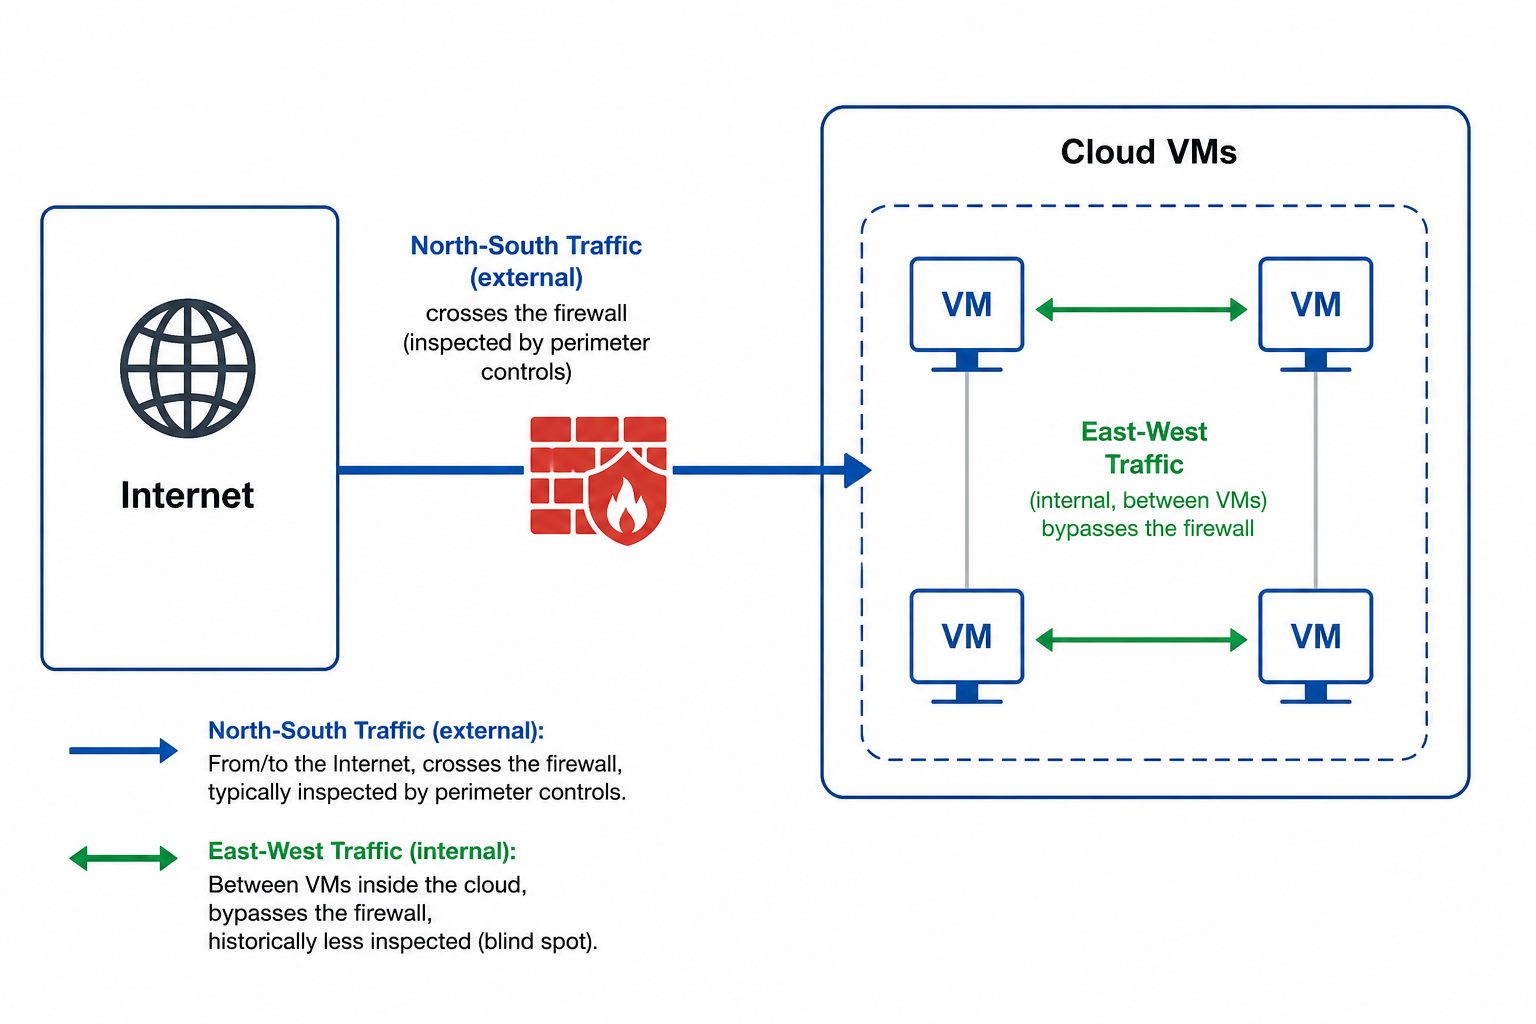
\includegraphics[width=0.82\textwidth]{figures/cloud_traffic_directions.png}%
  }{%
    \fbox{\parbox{0.75\textwidth}{\centering\vspace{1.2cm}
    \texttt{[Figure: cloud\_traffic\_directions.png, to be created]}\\[4pt]
    \small This is a simple original diagram (two boxes: ``Internet'' and
    ``Cloud VMs'', with a labelled arrow for north-south traffic crossing a
    firewall icon, and a separate labelled arrow for east-west traffic between
    VMs that bypasses the firewall). No external image needed, draw directly
    in PowerPoint, draw.io, or a tikzpicture.
    \vspace{1.2cm}}}%
  }
  \caption{North-south vs\ east-west traffic in a cloud environment}
  \label{fig:cloud_traffic}
\end{figure}


% Source for figure: draw it yourself or adapt from the NIST architecture diagrams
% at https://nvlpubs.nist.gov/nistpubs/Legacy/SP/nistspecialpublication500-292.pdf
% (NIST SP 500-292, open access, no copyright restrictions)

% ─────────────────────────────────────────────────────────────
\section{Security Challenges in Cloud Environments}
\label{sec:cloud_security}

The same qualities that make operationally attractive the cloud shared, scalable remote and API also represent the cause of its most severe security pitfalls. A systematic survey done by Alouffi et al. \cite{alouffi2021systematic} in the body of 80 reviewed articles about the safety of cloud found seven predominant classes of risks, with data leaking and manipulation and Unauthorized accessing occurring most often in those research articles surveyed. Next few subsections detail four kinds of risks primarily of network level intrusion detection significance.

\subsection{Misconfiguration}
It’s universally agreed that a significant portion of cloud security breaches is due to misconfiguration, the low-hanging fruit of open storage buckets, a too-generous firewall ruleset or disabled logging, all readily identified by automated scanners within minutes of their deployment. Cloud threat reports have also regularly listedmisconfigured services,insecure interfaces and weak access control as recurring vulnerability categories plaguing cloud users \cite{tabrizchi2020survey}.

The issue with misconfiguration is the effect of scale; if one IAM policy applied to 100 different instances and someone misconfigures it and all 100 will inherit the misconfiguration instantly. In a legacy environment, on prem misconfiguration could impact one or few servers but in the cloud, an individual misconfiguration could impact your entire data asset.

For IDS misconfiguration provides opportunity for compensating controls even the root issue is misconfiguration, IDS logs are able to capture the exploit of the misconfiguration once the hacker decides to exploit it, when hacker will scan a new exposed port or brute force against service that should never be exposed.

\subsection{Brute-force attacks on exposed services}

Any service that exposes itself externally to the internet over a network interface is susceptible to an automated credential attack against its exposed endpoint for example, port SSH (22), port RDP (3389), port database (5432), or port on an application web UI login page. In the cloud, every instance with a public IP address will be subjected to constant, automated attacks within minutes of it appearing on the public internet. 

Nadeem et al. Show that cloud networks are under perpetual attacks with constant automated brute force and DDoS attack attempts, and that IDS systems successfully interrupt many attacks when configured well \cite{nadeem2021intercept}. 

Brute force attacks result in a unique signature in terms of the volume of connection attempts targeting port Y on some destination device that originates from the same, or a small set of source IPs, with a higher ratio of attempted than completed successful connections. These signatures are readily detectable using flow level statistics, the primary features contained in the CICIDS2017 data set used in this investigation.

\subsection{Denial-of-service attacks}

DDos attack seeks to saturate server's resource bandwidth, CPU, connection table to make its unusable. Cloud elasticity protects against volumetric attack of DDos through bursting. A cloud can scale out the service and can accommodate high rate. But this service is limited, an excessive amount of volumetric attack will result in a great increase in service usage and consequently costs will go up due to the increase in the bandwidth usage.

The low rate application layer attacks, like RUDY, Slow loris, hold on to the established TCP connections with a small amount of data by a slowly increasing number of connections and are much harder to be detected. By holding the TCP connection to the server open with a small quantity of data, the attackers can successfully exhaust a server's resource and connection tables. Agrawal and Tapaswi in their research demonstrated that low-rate application-layer denial of service (DDoS) attacks (e.g. RUDY and Slowloris) have traffic characteristics close to normal slow clients, thus, difficult to detect through rate thresholds \cite{agrawal2019ddos}. 
Detection would probably require statistical approach and evaluation on the time windows.

\subsection{Lateral movement}

When a system is compromised, it by exploiting a vulnerable service, stealing credentials, or executing a phishing payload-an intruder will often perform lateral movement: exploring nearby systems within the network, also a virtual network, in an effort to increase their attack surface and gain access to additional resources or sensitive data. Since traffic that moves east to west generally avoids perimeter controls and analysis, the intruders' movement within an organization may go unnoticed for days or weeks. The MITRE ATT\&CK knowledge base, in its matrix dedicated to cloud environments, catalogues lateral movement as one of the core tactics of a cloud intrusion; the techniques it lists under this tactic include the reuse of stolen credentials and authentication material across services and the abuse of legitimate remote-management channels, usually preceded by internal discovery activity such as scanning for reachable services \cite{mitre_attack_cloud}. As internal traffic must be monitored for lateral movement attacks, internal visibility must be integrated into the design of any IDS.
Table~\ref{tab:cloud_threats} summarises the four threat categories and their key
detectable signatures.

\begin{table}[H]
  \centering
  \caption{Threats in cloud environments and their detection
           signatures in flow data.}
  \label{tab:cloud_threats}
  \renewcommand{\arraystretch}{1.4}
  \begin{tabularx}{\textwidth}{lXX}
    \toprule
    \textbf{Threat} & \textbf{Mechanism} & \textbf{Flow-level signature} \\
    \midrule
    Misconfiguration exploitation
      & Attacker targets an unintentionally exposed service
      & Rapid sequential port connections; unusual source geography \\
    \midrule
    Brute force
      & Automated credential guessing against SSH/RDP/HTTP
      & High connection count to single port; high failure rate; short sessions \\
    \midrule
    DDoS
      & Traffic flood (volumetric) or connection exhaustion (low-rate)
      & Abnormal packet rate or count; SYN flag anomalies; long session durations \\
    \midrule
    Lateral movement
      & Internal network probing and service exploitation after initial compromise
      & Unusual east-west flows; sequential internal port scans; new \\
        service-to-service communication patterns \\
    \bottomrule
  \end{tabularx}
\end{table}

% ─────────────────────────────────────────────────────────────
\section{Why Standard Security Tools Fall Short}
\label{sec:cloud_tools_limits}

The challenge with security appliances was that they were built around an era of networks with clear boundaries. A hardware firewall sits at the perimeter, an on-prem IDS sniffs the traffic going across the core switch. Neither idea translate to the cloud quite so neatly. 
In the cloud firewalls are really just named access control lists attached to each individual VM  security groups, not some centrally managed piece of hardware. 
And if your traffic between VM’s on the same host never makes it’s way across the physical network hardware, it won’t get seen by traditional network taps. While commercial cloud offerings from AWS GuardDuty and Microsoft Defender for Cloud address some of this, they only offer protection in a specific, proprietary cloud and they provide no access to the underlying logic. 
Running a private cloud on OpenStack or KVM ?
Good luck finding default detection tools there. 
It is precisely this gap which prompts the creation of an open and deployable ML based system to identify anomalous behavior across clouds using off the shelf components.

% ─────────────────────────────────────────────────────────────
\section{Summary}
\label{sec:cloud_summary}

Cloud computing itself is characteristically described by five qualities which are particularly security relevant; on-demand self-service makes it very easy for attackers to escalate quickly, widespread network access constantly offers a large attack surface for exposed services, resource pooling allows attackers to risk the security of other cloud occupants, elasticity makes constant static monitoring obsolete, and measured service makes useful logs available for event detection. As the infrastructure as a service, where the client is responsible for everything in the stack above the hypervisor, can impose the largest risk on security, we treat the Iaas as the most important service. In particular for Private and hybrid clouds, there’s a need for stand-alone detection tools, because the commercial “Cloud-Native” detection solutions don’t operate in these clouds. 

Three major attacks at the network level; brute-forcing, DDoS, and lateral movement, leave distinctive signatures on flow level, these signatures form our target in the detection system presented in this report and are present in the training and evaluation dataset. 
Chapter two: will provide a brief introduction of machine learning algorithms used for automatic recognition of those signatures.

%% ============================================================
%%  Chapter 2 - Artificial Intelligence and Machine Learning
%%  Simplified, no heavy formulas. All citations verified.
%% ============================================================

\chapter{Artificial Intelligence and Machine Learning}
\label{chap:ai}

\section{Introduction}

While "artificial intelligence" is quite broad, much of what people call AI in everyday language is a smaller subset: machine learning. Instead of someone sitting down and writing out a few if-then statements-"if this comes from this IP address and hits this port more than ten times a second, block it" we give a learning system a bunch of training examples and let it figure out the rule based on the data. This move from programmed logic to learning logic makes ML very powerful for tasks like intrusion detection. Attackers rarely declare their intentions upfront in a form that an rule-designer would recognize but they do create their traffic in a way that’s statistically regular, and the machine learning model picks up this pattern.
This section aims to remain mostly non-technical. I won't spend time on deriving the mathematics for each algorithm, but rather on providing enough background to fully understand Chapter~\ref{chap:ids}.
Section~\ref{sec:ml_types} discusses how the learning system is characterized by what it has learned from. 
Section~\ref{sec:ml_pipeline} explores the typical workflow. 
Section~\ref{sec:classical_ml} provides an overview of classical ML algos, those that predated and still inform deep learning, namely Random Forest (used here in baseline configurations). Section~\ref{sec:deep_learning} demystifies deep learning and why it became so dominant. We’ll end this section in Section~\ref{sec:xai} with an overview of explainability because making the model’s decision process clear to human eyes is another key goal of this project.

% ────────────────────────────────────────────────────────────
\section{How Machine Learning Systems Learn}
\label{sec:ml_types}

There is not simply “a way of doing“ machine learning. A variety of approaches can be taken, as we have seen, depending on your task and available data resources. A systematic review of the state-of-the-art by Alloghani et al. From 2020 analysed 84 research papers published between 2015 and 2018 and provided the key ML tasks categories: decision trees, support vector machines, and Naive Bayes was identified as the highest utilized supervised algorithms within these papers \cite{alloghani2020systematic}.

\subsection{Supervised learning}

With supervised learning, every data point in the training set also has an associated label a "ground truth" of the "right answer". If you are building a spam filter, each email in the training set is classified as either "spam" or "not spam." If you are building a brute-force attack detector, each flow in your training set will be labeled as "benign" or "brute-force." The training procedure for the model is to induce a pattern that connects the input (email or flow) to its correct classification, correcting it each time it fails to.

This methodology is pervasive in IDS research, primarily because datasets such as the CICIDS-2017 contain explicit labels, someone conducted attacks, generated traffic for each attack type, and then meticulously identified and logged which network flow was associated with which attack type \cite{sharafaldin2018cicids}. Without these annotations, the supervised learning approach simply has nothing to learn from.

\subsection{Unsupervised learning}
Unsupervised learning don't need labels. The model is simply provided with a set of data and asked to discover structures within this data, it should distinguish and cluster related data together, or detect data points that are significantly different from the main data pattern. In the context of network intrusion detection, this could mean the unsupervised model will learn how "normal" traffic appears to be and consequently identify any deviation from that pattern without receiving any beforehand information about the nature of an attack. 

While it is true that unsupervised learning can potentially discover novel attacks-which is indeed one of its undeniable merits, an idea further supported by Talaei Khoei and Kaabouch's comparison between unsupervised and supervised models with various intrusion detection data sets-the cost it has to pay in terms of performance is high \cite{khoei2023comparative}. 

Specifically, "different from normal" is not equivalent to "malicious". An unnormal but legitimate traffic spike might appear indistinguishable from a malicious attack from the model’s perspective, hence the relatively large rates of false alerts that are commonly associated with such models. This very reason why unsupervised learning is not the primary learning methodology of this project.

\subsection{A quick note on semi-supervised learning}

Of course there's a middle-ground: semi-supervised learning where a model is supplied with only a small pool of labelled data, but far larger amounts of unlabelled. The model uses the labelled examples to anchor and the unlabelled data to help flesh out its understanding. Mvula et al., in their 2024 survey of semi-supervised learning methods in cyber-security, explain semi-supervised learning as a direct response to what they see as a fundamental structural problem of our field: labelled traffic samples are difficult and costly to generate, while the volume of unlabelled traffic generated is enormous, and semi-supervised techniques make a reasonable attempt to exploit these resource disparities \cite{mvula2024semisupervised}. This is particularly pertinent in cyber-security where hand-labeling attack traffic relies on scarce, time-consuming expert human intervention.

% ────────────────────────────────────────────────────────────
\section{How a Model Actually Gets Built}
\label{sec:ml_pipeline}

We talk of training the model as if it were one step. The reality involves a sequence of rather tedious steps. Most of the actual work in an ML project involves activities which occur before the model ever gets to see any data at all.

\begin{enumerate}[label=\arabic*.]
  \item \textbf{Collect the data:} Which in our project, will include the CICIDS-2017 CSV files, along with some real traffic captured in lab.

  \item \textbf{Turn it into numbers:} No one can read a packet capture straight. The raw network traffic is first translated into a table of numerical features, such as the count of packets in the flow, duration of the flow, set flags, and many others. This process is named feature extraction and in this particular case, the feature extraction is done using CICFlowMeter, the tool which was used to generate the CICIDS-2017 features before.
  \item \textbf{Split the data:} Data splits into a train portion(this is what the model learns on) and a test set portion (a set kept back from the model, to test how it will generalize to data it hasn't seen). There are no hard rules here but usually, you will see a split of something like 70/30 or 80/20, depending on the volume of data you have to begin with.

  \item \textbf{Train:} The model goes through the training data multiple times, tuning itself each pass to minimize its errors. The specific details of "tuning itself" depend on the algorithm for Random Forests it means growing trees, for neural nets it means nudging around numerical weights.

  \item \textbf{Test:} After the training, the model is used on the test set that it didn't even touch during the learning process. This is the only just way to determine if the model truly understood, rather than just learning by memorising.

  \item \textbf{Deploy:} If the performance is adequate then the model goes in to real time deployment in this case classifying incoming live traffic streams as they are ingested.
\end{enumerate}

\subsection{How do you know if it's any good?}

After training a model, you're going to need some way to score it, and "accuracy" alone is a minefield. Umer et al, in a survey of ML-based intrusion detection for industrial control systems, note that IDS datasets are most always a skewed class problem: most of the time normal traffic forms over 90\% of the dataset, and so a classifier which labels every example as normal - without inspecting it - would get over 90\% just from accuracy \cite{umer2022ics}. CICIDS-2017 does indeed have this skew, so it becomes crucial to consider other measures.

These additional measures can be calculated from the four possible outcomes of a classification, illustrated in a confusion matrix in table \ref{tab:confusion_matrix}:

\begin{table}[H]
  \centering
  \caption{The four possible outcomes of a binary classification framed for IDS}
  \label{tab:confusion_matrix}
  \renewcommand{\arraystretch}{1.5}
  \begin{tabular}{ll cc}
    \toprule
    & & \multicolumn{2}{c}{\textbf{Actual traffic}} \\
    & & Attack & Benign \\
    \midrule
    \multirow{2}{*}{\textbf{Model says}}
      & Attack  & True Positive (TP) & False Positive (FP) \\
      & Benign  & False Negative (FN) & True Negative (TN) \\
    \bottomrule
  \end{tabular}
\end{table}

A false positive is an harmless flow that you have identified as a attack (in other words an alarm that should never have happened). A false negative is a real attack that you did not notice (a far more serious error from a security point of view).

\begin{itemize}
  \item \textbf{Precision : }  Of everything the model flagged as an attack, what was one? TP/(TP + FP). If precision is low there is a lot of false alarms
  
  \item \textbf{Recall : } (sometimes called detection rate) - how many of all the real
 attacks did the model detect? TP / (TP + FN). Low recall means attacks get through.
 
  \item \textbf{F1 score : } The single metric that finds the optimal sweet spot between precision and recall, a metric used for comparing models instead of trying to remember the 2 of them separately.
\end{itemize}

The measures of precision and recall typically come with an inverse relationship with each other: tune a model to catch more of the attacks (high recall) and it will be likely to classify many legitimate activities as attacks too (low precision). This tradeoff depends on the particular use-case rather than pure math; when using an intrusion detection system (IDS) missing real attacks are often deemed worse than a few false positives, but high false positives can make analysts tune out altogether \cite{umer2022ics}.

% ────────────────────────────────────────────────────────────
\section{Classical Algorithms: Trees and Forests}
\label{sec:classical_ml}

In days before deep learning took center stage, several very simple algorithms were responsible for most of the effort put forth in applied machine learning, and many still continue that task not because they have historical significance as predecessors, but because they work they are efficient, they’re understandable, and oftentimes just as accurate as models that are magnitudes more complex. This is not simply an argument based on practicalities: A comparative controlled test of DL and classical models, conducted in 2025, comparing model performance on network intrusion data shows CNN and LSTM models perform about 98\%, whereas a Random Forest performing the exact same task achieved a 99.9\% score; classical models perform better here \cite{ali2025dlvsml}. While the result of course depends on the specific problem and dataset, it’s a concrete outcome that’s very common in the literature, and one reason that we can see a Random Forest model as a first pass approach and not a “compromise”.
 
\subsection{Decision trees}
 
A decision tree acts as it sounds, you’re asking a series of questions of the input, and based on the answer you traverse one path in the tree to another question, until you eventually come to a conclusion: “Is the destination port 22? If yes, do I have more than one connection attempt per second from this source? If yes, flag brute force.” The decision tree idea itself originates from Quinlan’s ID3 algorithm, which in essence builds a tree, each step of the way, selecting the question that best separates the available examples into their respective categories \cite{quinlan1986id3}.
 
What a thing like this looks like is illustrated in a simplified manner in figure~\ref{fig:decision_tree} for a type of decision like those that our project’s IDS must make.
 
\begin{figure}[H]
  \centering
  \IfFileExists{figures/decision_tree_example.png}{%
    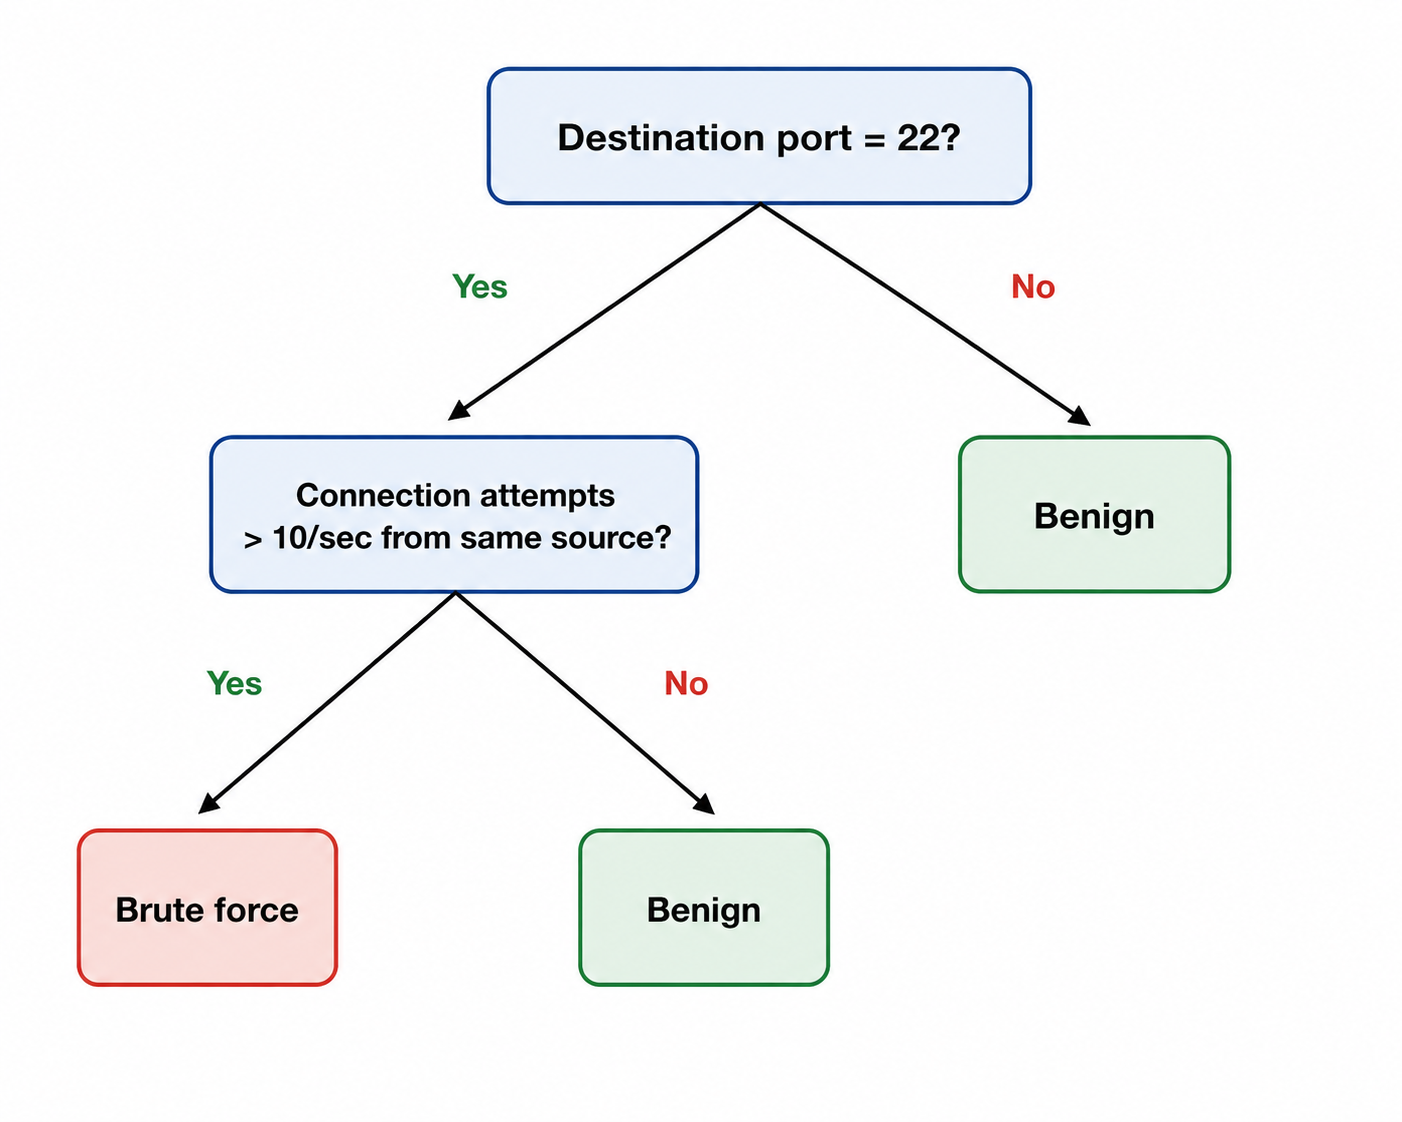
\includegraphics[width=0.75\textwidth]{figures/decision_tree_example.png}%
  }{%
    \fbox{\parbox{0.78\textwidth}{\centering\vspace{1.2cm}
    \texttt{[Figure: decision\_tree\_example.png, to be created]}\\[4pt]
    \small A simple original diagram: a root node asking "Destination port = 22?",
    branching to a node asking "Connection attempts $>$ 10/sec from same source?",
    branching down to two leaf nodes labelled "Brute force" and "Benign." Draw
    directly in draw.io, PowerPoint, or a tikzpicture, no external image needed.
    \vspace{1.2cm}}}%
  }
  \caption{Simplified decision tree for flagging SSH brute-force traffic}
  \label{fig:decision_tree}
\end{figure}
 
What is nice about a single tree is that you can literally just read it to see exactly why each decision was made. What is unfortunate, as identified by Quinlan himself in a discussion of the approach, is that because a tree built greedily one split at a time can never “undo” a mistake it made early on when it’s able to see more data \cite{quinlan1986id3}, it can sometimes be “overfitted” to peculiarities of its particular training set, so that tiny changes in training data result in a considerably different tree.
 
\subsection{Random Forest}
 
The Random Forest overcomes this instability by training multiple (often several hundred) trees instead of one and averaging over their predictions. To train each tree, we either use a slightly different random sample of the training data, or we randomly constrain the set of features to use at each split. In the paper that introduced the algorithm, Leo Breiman described the forest as a collection of tree predictors where each tree is grown from its own independently sampled random vector, and he proved that the generalization error of the ensemble settles towards a limit as more trees are added rather than growing worse -- adding trees cannot overfit the forest \cite{breiman2001random}.

We represent this concept schematically in Figure~\ref{fig:random_forest}: the flow through a number of similar-looking trees is run, and the result is the one which receives a majority vote among all the trees.
 
\begin{figure}[H]
  \centering
  \IfFileExists{figures/random_forest_voting.png}{%
    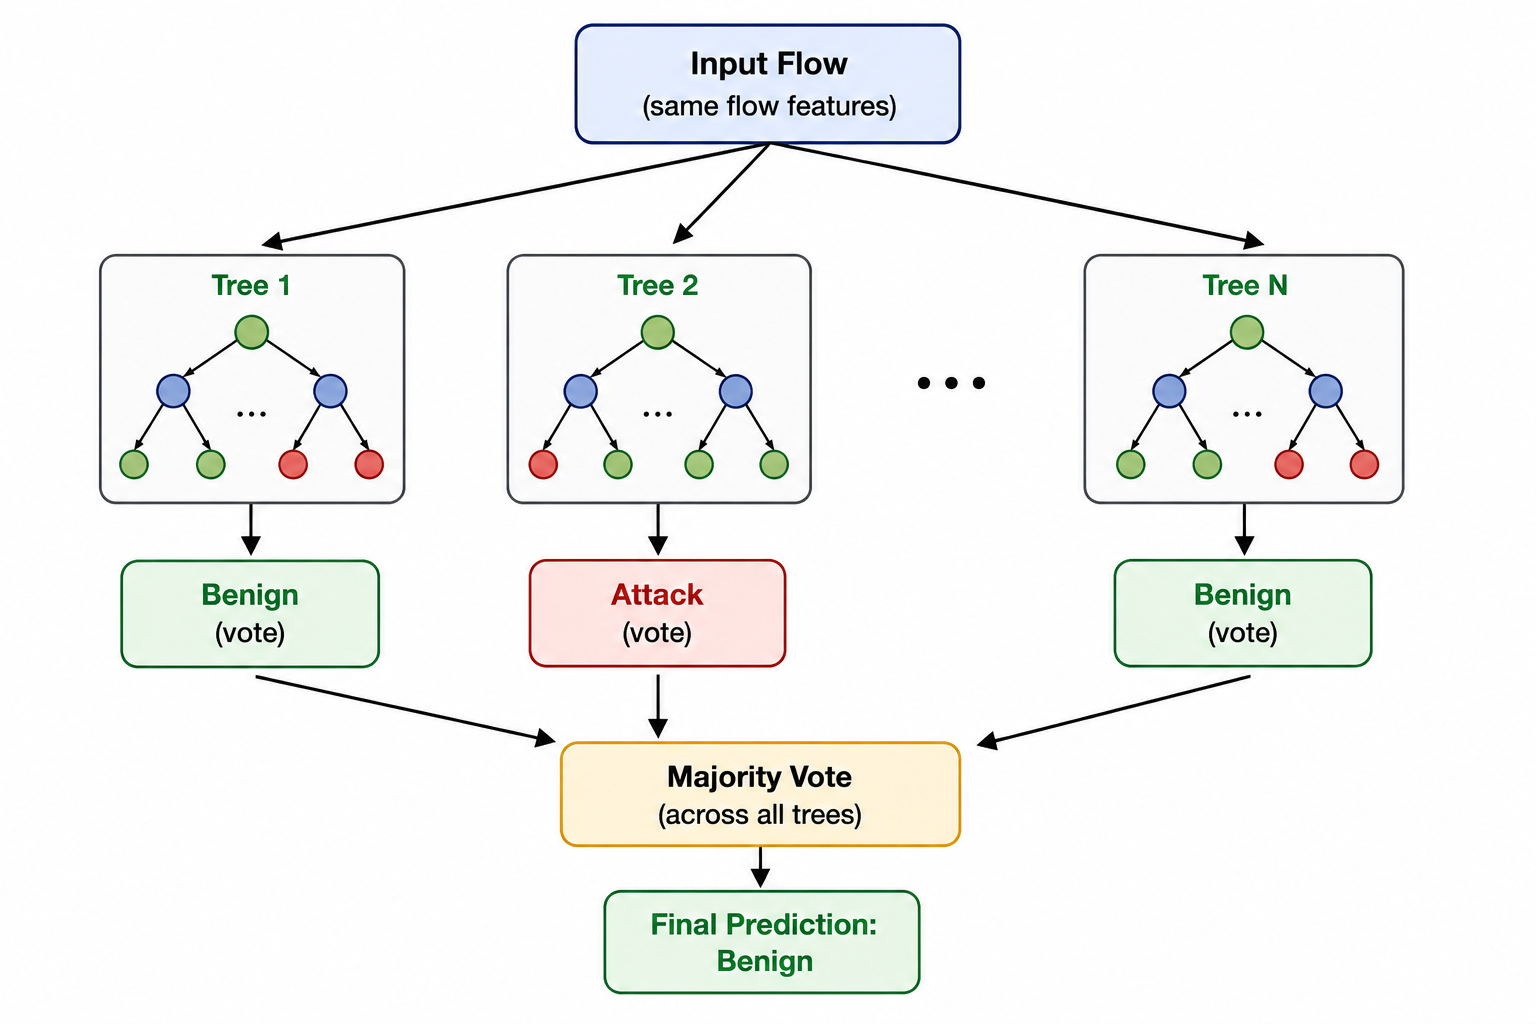
\includegraphics[width=0.8\textwidth]{figures/random_forest_voting.png}%
  }{%
    \fbox{\parbox{0.78\textwidth}{\centering\vspace{1.2cm}
    \texttt{[Figure: random\_forest\_voting.png, to be created]}\\[4pt]
    \small A simple original diagram: one input flow at the top, an arrow fanning
    out to several small decision-tree icons (Tree 1, Tree 2, ... Tree N), each
    producing its own Attack/Benign vote, all arrows converging into a single
    "Majority Vote" box at the bottom producing the final label. Draw in draw.io,
    PowerPoint, or a tikzpicture.
    \vspace{1.2cm}}}%
  }
  \caption{How a Random Forest reaches a decision \cite{breiman2001random}.}
  \label{fig:random_forest}
\end{figure}
 
Randomness is what matters, by making the trees less correlated with each other, we ensure that the error of any particular tree has a tendency to be offset by the errors of the others, which is more helpful for the result as compared to those errors accumulating over the ensemble of trees, ultimately yielding a classifier that performs at about the same speed and is as interpretable as a single decision tree while having the advantages of both increased robustness and accuracy. Besides this, Random Forest is capable of producing feature importance scores that rank features by how they contribute to the overall accuracy of the classifier which is useful for identifying drivers for detections, something that will be addressed again in Section~\ref{sec:xai}. Therefore, Random Forest will be our base classifier, although not as advanced as other techniques, it represents a sound choice due to the good trade off it presents in terms of complexity, speed and interpretability. The choice also sits on familiar ground: the decision trees a forest is built from were found by Alloghani et al. \cite{alloghani2020systematic} to be among the most implemented and discussed supervised learners in the applied literature.

\subsection{A brief word on other classical methods}
 
There are two other algorithms that appear frequently enough in the IDS literature that are worth mentioning very briefly. The Support Vector Machine \cite{cortes1995svm}, which was pioneered by Cortes and Vapnik, maps the input data into a higher-dimensional space and finds the smoothest possible separating plane which divides the two class labels with the largest possible margin. The k-Nearest Neighbour \cite{cover1967knn}, which is among the oldest rules for classification, works by going over all of the training examples already seen and determining the label of the ones that most closely resemble the new input data. Although both techniques are of interest, neither is a key component in this work, so they aren't addressed in any detail in the remaining chapters.
 
% ────────────────────────────────────────────────────────────
\section{Neural Networks and Deep Learning}
\label{sec:deep_learning}

“Deep” just means deep in a literally visual sense of stacking dozens or more levels of simple compute on top of one another, where each layer process input from the previous layer just a little and after passing through many such layers the data eventually is being described in a format where making the final choice is easy.   LeCun, Bengio, and Hinton, in a summary designed for a broad scientific audience, summarized it quite aptly: for supervised deep learning of the typical kind, a device is fed many instances with an associated label, outputs a value corresponding to each possible classification label, and fine-tunes its parameters every time the score does not correspond to the label \cite{lecun2015deep}. For a general neural network for classification, this applies to nearly everything in terms of image or network flow classification.
 
\subsection{Why neural networks took over}
 
The simple answer: scale. Machine learning approaches that are good with structured, already organized data the tabular structure of the CICFlowMeter output, for example are more straightforward: models like Random Forest can learn relationships that the provided table implicitly describes. Neural nets, on the other hand, are much more at home dealing with something more closely resembling raw input: you can feed a net raw pixels from an image or a stream of values, and it can learn the relevant characteristics on its own. 

LeCun, Bengio, and Hinton refer to it this way: rather than designing a feature extractor using domain knowledge to identify what information to extract for an input (for example, a dog image is useful if you look for ear shapes and dog nose), representation learning can find the right representation for an input automatically \cite{lecun2015deep}. 

When there was enough data, enough compute power and enough interest in training networks this way, it was the power of these nets to find their own relevant features that enabled rapid advances in areas like image recognition, after a 2012 paper radically reduced the error rate of a popular image benchmark \cite{krizhevsky2012imagenet}. We’ve since been trying to apply those same advances to network data.
 
\subsection{Convolutional networks}
 
CNN (Convolutional Neural Network): is a type of neural network, not scanning every individual input value separately, but scanning for small patterns locally in the input. In a word from O'Shea and Nash's tutorial, the same little filter is moved all the way over the input. So as soon as that local pattern appears on the image anywhere the same filter recognizes it. The network doesn't have to relearn that same pattern independently in every different location, and this is where much of the CNN’s effectiveness in image-based tasks comes from \cite{oshea2015cnn}” Although this structure is motivated by images, it maps perfectly to network data, where a pattern would appear as a short burst of unusual packet flow.

\subsection{Sequence aware networks}
 
Network traffic is not simply a bunch of unrelated flow requests-the order that flows happen often is meaningful. A “slow” port scan doesn’t result in any single flow request of significant size; it only looks out of the ordinary when you analyze a series of such flows over time. Sequence modeling architectures, most importantly LSTMs (Long Short-Term Memory), do carry information between steps. 

As proposed in 1997 by Hochreiter and Schmidhuber \cite{hochreiter1997lstm}, the architecture helps deal with the tendency of many-steps-ago information to vanish before affecting a future step’s decision by using its “gates” mechanism that allow useful information to be maintained. 

An architecture like the CNN presented here is not able to retain memory this way; however, you should know this architecture as it has been used in some systems such as the ones in Chapter~\ref{chap:ids}.

\subsection{The trade-off neural networks bring}
 
However, none of this is without cost. Neural networks tend to require significantly more training data to get anywhere close to top performance, also tend to take significantly longer to train and, most importantly for the purpose of this project, tend to be much harder to interpret. A Random Forest might be able to provide you with a sense for why the decisions were made, whereas the inner workings of a neural network is (out of the box) a mystery. Table~\ref{tab:classical_vs_deep} summarizes this compromise more quantitatively.
 
\begin{table}[H]
  \centering
  \caption{Classical machine learning vs.\ deep learning}
  \label{tab:classical_vs_deep}
  \renewcommand{\arraystretch}{1.4}
  \begin{tabularx}{\textwidth}{lXX}
    \toprule
    \textbf{Factor} & \textbf{Classical ML (e.g.\ Random Forest)} & \textbf{Deep
      learning (e.g.\ CNN, LSTM)} \\
    \midrule
    Data to be trained & Performs best on medium sized labeled data sets &
      Usually requires a significantly bigger data set to be effective \\
    Feature engineering & Needs features pre-computed (ex: using CICFlowMeter) & Can extract useful information from minimally processed data \\
    Training time & Fast minutes on a standard CPU & This typically takes several hours, although requires a GPU for training in a practical time frame. \\
    Interpretability & High decision paths, feature importance directly visible & Low by default: you have to add another Explainable Method (e.g. SHAP). \\
    Traditional IDS applications & Good as a strong baseline; works well for \\
    flow-level tabular features. & Better for sequential attacks / attacks over time \\
    \bottomrule
  \end{tabularx}
\end{table}
 
The training-data and training-time rows are what Ahmad et al. Noticed about the deep learning IDS work they reviewed-that deep models usually had GPU test beds, sizable data-sets, and comparable accuracy \cite{ahmad2021network}. The interpretability row is a key insight from Lundberg and Lee: the most accurate models on sizable data-sets often are precisely the models most difficult for a person to interpret \cite{lundberg2017shap}. No row is definitively "better"-they’re appropriate in different parts of the process and it’s the value of that trade-off which has given rise to explainability methods, introduced next.

\section{Making Model Decisions Understandable}
\label{sec:xai}
 
A system that achieves 99\% accuracy but provides no explanation for any of its classifications is of limited value to security professionals. If the system determines a connection is malicious, for instance, the analyst will require some understanding of why the connection was deemed malicious before acting on it, whether that’s by blocking a particular IP, escalating an incident to the next level, or dismissing the alert as a false positive. The exact same dilemma is articulated in the context of intrusion detection systems (IDS) in the 2025 systematic literature review on XAI adoption in IDS by Mohale and Obagbuwa, who point out that many of today’s most accurate IDS are black boxes, obscuring the reasons behind alerted events and hampering analyst trust in these systems \cite{mohale2025xaiids}. This practical impediment is precisely what lies behind XAI, and is highly pertinent to the objectives of this research of developing an explainability layer within the detection workflow.
 
\subsection{The problem in plain terms}
 
Lundberg and Lee pose the problem most directly: The top accuracy on large, modern
datasets usually come from models that people are the least capable of interpreting, which generates a tension between model performance and human interpretability \cite{lundberg2017shap}. You wouldn’t get from hundreds of trees in a Random Forest, or millions of internal parameters in a neural network, a one-sentence answer explaining any single prediction. You have to apply something else on top, after the fact.
 
\subsection{SHAP values}

The method the project employs is called SHAP (SHapley Additive exPlanations). This concept is adapted from a far older game-theory method that helps you to divide the credit among individuals who worked to achieve some collective result. SHAP implements this for the features of a model and, for any given prediction, computes the extent to which each input feature has shifted the result towards the output "attack" class (and away from "benign"), summing exactly to the final prediction \cite{lundberg2017shap}.

This translates, in a practical sense, to this system not simply reporting an alert: if the detection system alerts that a flow is malicious, then in addition to the classification, it will explain precisely why: the flow was flagged because the number of SYN packets was far higher than normal and the connection was far shorter than normal, for example. This ability to decompose why an alert has occurred is how one can transition a black box to a set of decisions a security analyst can meaningfully make and that is the main contribution here.
% ────────────────────────────────────────────────────────────
\section{Summary}
 
Replacing hard coded detection rules with data derived patterns comes in the form of machine learning where a particular flavour will depend on whether you can provide examples with expected outputs (supervised learning) or you cannot (unsupervised learning). There’s quite more to building a functional model than just training it. You will need to collect data, turn it into meaningful features, partition the data for testing, and finally assess the models with metrics that actually have a real bearing on the problem, which in this case means high recall and precision (not accuracy).

My default model, given its speed, familiarity, and truly decent performance (even without tuning) is an ensemble of decision trees, aka a Random Forest. I would like to explore a few Deep Learning solutions, a Convolutional Neural Network (CNN), and a “time aware” one, called Long Short-Term Memory (LSTM), which will most likely require a higher volume of training data but has also proven capabilities for this problem. SHAP value can bring back interpretability lost in those deeper models.
Based on that foundations I will explore the different machine learning approaches to network intrusion detection, focusing on what works and what doesn’t and where is there space to improvement that my projects hopes to address.
  
%% ============================================================
%%  Chapter 3 - Intrusion Detection Systems: State of the Art
%%  All citations verified (DOIs via doi.org / publisher pages).
%%  Label chap:ids resolves the two pending Chapter~\ref refs
%%  in chapters 1 and 2.
%% ============================================================

\chapter{Intrusion Detection Systems}
\label{chap:ids}

\section{Introduction}
\label{sec:ids_intro}

An IDS is simply a watching eye. An IDS monitors network traffic or activity on a host and checks for potential threats; it issues an alarm if it finds any but does not block it. So it has to make sound judgments; any alarm raised in response to an incident has zero value if there is a significant delay in delivering it, if the details provided lack context or are simply one in hundreds of non-issues. 
This chapter provides a review of what’s already available. 
We examine three main types of solutions; signature based which are most popular in production; the managed detection offered by cloud vendors; and ML algorithms in development. For each we evaluate how well they do against the cloud threats described in Chapter \ref{chap:cloud}. We assume knowledge of the algorithms discussed in Chapter \ref{chap:ai}. Then we summarize the missing links when all three are evaluated; we then explain how the developed system fills those gaps.

% ─────────────────────────────────────────────────────────────
\section{Two Detection Philosophies}
\label{sec:ids_philosophies}

But ultimately, there are just two ways for a system to tell that traffic is malicious: Signature-based detection (which in the literature, is often shortened to SIDS.) The system maintains a database of attack patterns that have been previously observed and analyzed, comparing all incoming traffic to that database. If a pattern match occurs, an alarm is issued. 

In their famous survey of intrusion detection techniques, Khraisat et al.\ point out that SIDS has a high accuracy on past intrusions but is inherently limited: if an attack is not present in the signature database, there can be no match, and if there is no match, there can be no alert-in other words, zero-day attacks get through precisely because nobody has ever created signatures for them \cite{khraisat2019survey}. 

The second method is anomaly-based detection (AIDS by the same terminology). This technique builds a profile of normal activity and marks anything that deviates from that profile rather than relying on a catalog of known attacks. The upside is the inverse of SIDS: zero-day attacks are still caught, because you don’t have to know what the attack is, just that it is atypical. The disadvantage is also the inverse of SIDS: anomalous activity but non malicious activity will deviate from the normal profile just as much as an attack would, resulting in those false positives for which anomaly detectors are infamous \cite{khraisat2019survey}. 

In this context, machine learning is the most popular modern method of building that model of normalcy (or, in supervised models, a separate model for each attack type), accordingly, almost all of the papers we survey later will be of this variety. 

SIDS and AIDS aren’t exactly in competition, mature deployments almost always include both. Nevertheless, they both fail, just in different ways, and in ways that inform which type is best for you.

% ─────────────────────────────────────────────────────────────
\section{Signature-Based Tools in Practice}
\label{sec:ids_signature}

But the tools in actual use on the majority of networks today? They’re signature based. Snort, a venerable network IDS that dates back to the late 90s and its younger, multi-threaded counterpart Suricata, all function the same way at the base level: a rule set document dictates what the patterns look like, the constraints that can be imposed on the source/destination of traffic, which ports to look on, and content to be seen inside packets, and the engine matches network traffic against thousands of such patterns. 
It’s an effective method for many of the best reasons: rules are easily readable for an analyst and provide precise context. 
Known maliciousness can be detected quite rapidly. And the rule making environment is well developed with the open source community, vendors, and security intelligence firms regularly releasing new or updated rule sets.


How badly does this approach miss what it doesn't know?
Holm found out exactly that when he launched 356 serious attacks against a Snort that used an official rule set old enough for 183 of those attacks to have come after it, meaning they were legitimate zero-days to Snort \cite{holm2014signature}. And it works both ways.
It's not as though Snort was stone deaf, it caught 17\% of zero-day attacks (usually because the new ones looked somewhat similar to ones it knew) \cite{holm2014signature}.
But after testing how fragile those catches were, Holm concluded with a conservative estimate that the true zero-day detection rate was 8.2\%, while Snort caught 54\% of the attacks the signatures were designed for. In crude terms, nine out of 10 zero-day attacks fly under the radar. And almost one in two known attacks slip past if Snort's rule set has become outdated.


On top of that there's an ongoing cost: the signatures don't just exist, they have to be authored by humans. Every variant means a new rule set and rule sets have to be updated and tested against false positives as traffic and malware patterns shift a never-ending specialist job \cite{khraisat2019survey}. Add to that the cost implications of a cloud infrastructure where traffic that flows east-west (Chapter~\ref{chap:cloud}) isn't visible to a perimeter appliance at all and you can see why the "perfect rule set" is a pipe dream.

% ─────────────────────────────────────────────────────────────
\section{Commercial Cloud-Native Detection}
\label{sec:ids_commercial}

The main cloud vendors offer their own solution for this issue. AWS GuardDuty, Microsoft Defender for Cloud and Google Security Command Center leverage the cloud vendor’s telemetry, network flow logs, API call data, DNS traffic and apply rules, combined with a certain dose of proprietary ML against it. Within their own infrastructure, these tools are in fact quite effective, have access to sources others can not, and have practically no overhead for configuration.
Three limitations are relevant to this project:

An organization managing an OpenStack / KVM based private cloud like the one in Section~\ref{sec:deployment_models} has nothing it can even enable, same for the private part of a hybrid environment. The places that potentially need tooling the most are exactly those which these tools do not reach.

Second, opacity. The detection logic isn’t exposed. When GuardDuty generates a finding, the analyst is informed of what triggered the alert, but not why it triggered the alert; when the finding is incorrect, there’s no model to investigate or alter. 
Indeed, even AWS’s documentation recognizes this workflow dynamic by offering suppression rules-a feature to automatically archive findings the user has determined to be expected behavior instead of a threat \cite{aws_guardduty_suppression}. 
Suppression deals with the symptoms; it conceals false positives, but doesn’t justify them or resolve them.

The third follows on from the second: the effort of tuning. Training on generically behaving activity often flags activities which should happen in a given environment: scheduled scans, NAT gateway traffic, CI/CD pipelines, etc. Each of those leads to analyst effort until a suppression rule takes effect. 
All that doesn’t mean those commercial products are bad, though. They mean that they are neither accessible in a private cloud nor transparent anywhere else, the very two things that this project addresses by attempting to provide an open-source alternative.


% ─────────────────────────────────────────────────────────────
\section{Machine Learning Approaches in Research}
\label{sec:ids_ml}

We have been exploring and demonstrating the application of learning algorithms for intrusion detection for over two decades and largely the rationale for such research has been to try to overcome the signature trap. There is a great deal of research and we can organize it broadly around paradigms, restricting the summary below to that which each paradigm can demonstrably achieve; the underlying workings of the learning algorithms can be found in Chapter~\ref{chap:ai}. Table~\ref{tab:ids_taxonomy} gives the overview.

\begin{table}[H]
  \centering
  \caption{Families of ML/DL approaches in academic IDS research.}
  \label{tab:ids_taxonomy}
  \renewcommand{\arraystretch}{1.4}
  \begin{tabularx}{\textwidth}{lXX}
    \toprule
    \textbf{Family} & \textbf{Representative techniques} & \textbf{Demonstrated strengths / recurring limits} \\
    \midrule
    Classical supervised ML
      & Decision Trees, Random Forest, SVM, k-NN
      & Excellent accuracy on flow features; fast to train and run;
        depends on engineered features and labelled data \\
    \midrule
    Supervised deep learning
      & DNN, CNN, RNN/LSTM, hybrid CNN--LSTM
      & Learns features from raw or minimally processed input;
        strong on sequential attack patterns; data- and compute-hungry \\
    \midrule
    Unsupervised / generative
      & Autoencoders, VAE, GAN
      & No attack labels needed, can surface novel attacks;
        higher false-positive rates than supervised models \\
    \midrule
    Emerging directions
      & Transformers, LLMs, few-shot / meta-learning
      & Model long-range dependencies; address label scarcity;
        interpretability and computational cost remain open problems \\
    \bottomrule
  \end{tabularx}
\end{table}
 

\subsection{Classical machine learning}
\label{sec:ids_classical}

The most established and still strongest category of work consists of training classical models, like Random Forest, SVM, k-NN, or decision trees, on the same flow-level features produced by CICFlowMeter. In this work, results on benchmark data are solid: the controlled study in Ali et al.\ mentioned earlier in Section~\ref{sec:classical_ml} already showed tree-based models outperforming the deep learning counterparts on the exact same classification task \cite{ali2025dlvsml}. Systematic surveys on this problem set also arrive at a similar conclusion: classical approaches do very well given appropriate features, and their sole major dependency is precisely those very features and availability of labeled data \cite{ahmad2021network}. Novelty generalization is their weaker point, and a model trained on yesterday's attacks doesn't particularly have reasons to identify tomorrow's.

For this project, that trade-off works in our favour. The CICIDS-2017 features are already computed and the data already labelled, so the expensive part is done. A Random Forest baseline is cheap to train, fast at inference, and transparent enough for its output to feed an explainability layer. That is why Chapter~\ref{chap:cloud} and Chapter~\ref{chap:ai} already pointed to it as our base model.

\subsection{Supervised deep learning}
\label{sec:ids_deep}

The latest waves to crash onto the shore of intrusion detection come on the back of the promise made in Section~\ref{sec:deep_learning} of having to bother with feature engineering never again, learn it all direct from the data. We get the usual candidates in the survey papers of these models; the deep feed forward networks, the CNNs who learn images of flow matrices or byte streams of the payload, the LSTMs working on flow sequences and a variety of hybrid approaches combining the spatial awareness of a CNN with the temporal memory of a LSTM \cite{kimanzi2024deep, ahmad2021network}. The performance on the standard datasets such as the CICIDS-2017 family are high, not dissimilarly to the well established approaches. Of course the familiar worries of Chapter~\ref{chap:ai} appear enormous volumes of labelled training data, massive GPU needs, non interpretable results \cite{ahmad2021network}. And inevitably when they compare there results with ensembles there is only marginal gains in accuracy \cite{ali2025dlvsml} and little advantage for there models over classic methods for flow table features except for sequential type attacks (scans and low rate flooding) .

\subsection{Unsupervised and generative approaches}
\label{sec:ids_unsupervised}

A different thread drops the labels altogether. Autoencoders are trained to compress and reconstruct normal traffic. If a flow is badly reconstructed by the model, it must, by definition, be unlike anything that the model saw during training and is therefore declared abnormal. 
Generative adversarial networks (GANs) go even further: the model learns explicitly what constitutes the distribution of normal behaviour \cite{kimanzi2024deep}. 
Once you have read Section~\ref{sec:ids_signature}, the benefit should be apparent: none of these techniques assumes foreknowledge of the attack, so these research communities offer the most straightforward solutions to zero-day threats.

The cost is one which Chapter~\ref{chap:ai} had already highlighted for unsupervised learning in general. “Different from normal” is less strong evidence than “similar to a known attack”, and studies that compare supervised and unsupervised models on intrusion datasets found the unsupervised models pay a price for their flexibility by delivering lower precision and higher false alarms compared to their supervised cousins \cite{khoei2023comparative}. In practice each of those false alarms has to be triaged by an analyst.

\subsection{Emerging directions}
\label{sec:ids_emerging}

Two frontier directions are worth a brief call-out here - in part for completeness, in part to illustrate what this project does not try to achieve. The role of transformers and of large language models (LLMs) in NLP is making an impact into the threat-detection space. A recent review from Kheddar discusses how attention based models, BERT based encoders, GPT based generators, and vision transformers were re-purposed for intrusion detection, showing great potential in modelling long-range dependencies in traffic, and highlighting challenges related to explainability, scale and adaptability in response to evolving attacks \cite{kheddar2025transformers}.

Alternatively, other work takes an offensive stance and tries to attack directly the issue of scarcity in labels. Few-shot and meta-learning models are aimed to detect an attack class in presence of only a few examples of the attack instead of thousands of examples, and methods such as the framework NERO combine neural algorithmic reasoning and metric-based meta-learning for the identification of zero-day attacks in IoT traffic under exactly those low-label conditions \cite{cevallos2024nero}.

Both of those are valid and interesting context, neither of which we follow here, they trade the problems we do care about (transparency, deployability on humble hardware) for abilities we don't need.
% ─────────────────────────────────────────────────────────────
\section{Gap Analysis}
\label{sec:ids_gaps}

Set the three families beside each other, and you notice four cracks that branch from them. Each one is rooted in something concrete, either in this chapter or in the two before it.

\textbf{Gap 1: novel attacks defeat the deployed tools.} The actually production-used detection tools are the signature engines, and the data show that they miss the large majority of the attacks for which they don’t have any rule \cite{holm2014signature}. Learning-based detection is supposed to address this in principle, but usually just within research papers, not in operational tools.

\textbf{Gap 2: nothing to deploy in a private cloud.} The commercial detection services only run inside their own platform, and they reveal nothing about their logic anywhere. For the OpenStack or KVM operator of Section~\ref{sec:deployment_models}, and the private part of any hybrid deployment, there’s nothing equivalent in turn-key fashion, and the environments this project targets are precisely these.

\textbf{Gap 3: the accurate models are the opaque ones.} Throughout the body of work, detection performance and interpretability pull in opposing directions; the trend Lundberg and Lee noted in general \cite{lundberg2017shap} and which Mohale and Obagbuwa illustrate in the case of IDS, whereby black-box alerts undermine the trust that the system, whose alerts they are, exists to support \cite{mohale2025xaiids}. Few of the published systems present the explanation alongside the alert.

\textbf{Gap 4: evaluation stops at the benchmark.} As described above, virtually all the papers studied perform evaluation on pre-extracted static feature files, with a CSV to train, another CSV for the holdout, and reporting a single score \cite{ahmad2021network, ali2025dlvsml}. That is the proper way to compare models, but an actual IDS has a harder job: processing a live stream of traffic, extracting features on the fly and classifying within latency limits. This last part is where most papers stop, leaving it as future work.

The four gaps are being closed by the system that follows this chapter: an anomaly-capable ML detector (Gap 1); open and runnable on commodity virtualisation (Gap 2); with a SHAP explanation linked to each alert (Gap 3); and, for Gap 4, an evaluation that deliberately goes beyond the static benchmark to independently generated traffic, with the live-pipeline deployment designed and its feasibility established rather than merely assumed.

% ─────────────────────────────────────────────────────────────
\section{Summary}
\label{sec:ids_summary}

Signature-based systems remain the most deployed forms of intrusion detection, and they are fundamentally blind to anything that they haven't already observed, hence measured zero-day detection rates in the single digits to high teens of percent. Cloud provider-managed services do a reasonable job within their own ecosystem, are absent from private infrastructure, and provide no transparency at all. Academic ML reduces the gap on paper ensemble methods, for instance, remain competitive with deep networks on flow data but it preserves the black-box problem and has, largely, never left the established benchmarks. We have thus found four key shortcomings: novelty, deployability, explainability, and liveness, which we deal with in detail in Chapter~4.
  
%% ============================================================
%%  Chapter 4 - Conception of the Proposed System
%%  Raw commands/configs deferred to
%%  Chapter 5 and the annexes, per the template rule.
%%  Only external citation needed here: sharafaldin2018cicids.
%% ============================================================

\chapter{Conception of the Proposed System}
\label{chap:conception}

\section{Introduction}
\label{sec:conception_intro}

I finished up the last chapter highlighting four areas in which the existing intrusion detection landscape left something to be desired. In fact, the entire design of this project revolves around those very areas: that this project must detect attacks that it has not explicitly been coded for (Gap~1), that it will be deployed in a private cloud using commodity hardware and will not be reliant upon a commercial provider platform (Gap~2), that this project must present understandable reasons for its alerts to users, not simply identify threats as they occur (Gap~3) and that the solution will operate in a low-latency, time-constrained environment handling live traffic rather than offline, batch processing of historical data (Gap~4).

The following chapter describes how those four requirements lead to a real-world design, covering: the overall architecture of the system, the decision to model a real-world private cloud using a virtual two-machine lab, the justifications for key environmental decisions, the dataset, the approach to the dataset's features, and the method of training and choosing a detection model. The focus of this chapter is primarily \emph{what} we decided to build and \emph{why}. The building itself the exact commands, the configuration files, and screen captures of the system running  together with its measured outcomes, will be addressed in Chapter~\ref{chap:results}. Where choices involved tradeoffs, alternative directions which were not taken are also described, for the alternative paths in a project such as this are generally as informative as the successful one.

% ─────────────────────────────────────────────────────────────
\section{Overall Architecture}
\label{sec:conception_architecture}

At the highest level the system is a pipeline of four stages, each feeding the next. Traffic is \textbf{captured} from the network, converted into \textbf{flow features}, passed to a \textbf{detection} model, and any alert is then \textbf{explained and surfaced} to an analyst. Figure~\ref{fig:architecture} shows the arrangement.

\begin{figure}[H]
  \centering
  \IfFileExists{figures/system_architecture.png}{%
    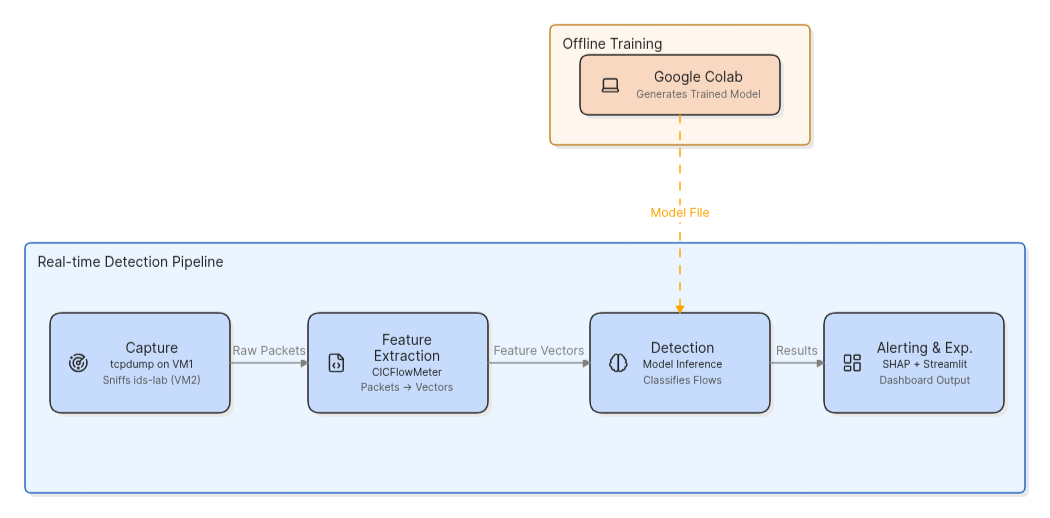
\includegraphics[width=0.92\textwidth]{figures/system_architecture.png}%
  }{%
    \fbox{\parbox{0.85\textwidth}{\centering\vspace{1.2cm}
    \texttt{[Figure: system\_architecture.png  to be created]}\\[4pt]
    \small Original block diagram of the four-stage pipeline. Left to right:
    (1)~\textbf{Capture}  attack traffic from VM2 crossing the \texttt{ids-lab}
    network, sniffed by \texttt{tcpdump} on VM1; (2)~\textbf{Feature extraction}
     CICFlowMeter turning packets into flow feature vectors;
    (3)~\textbf{Detection}  the trained model classifying each flow;
    (4)~\textbf{Alerting \& explanation}  SHAP annotating the alert, intended
    for presentation on an analyst dashboard. A separate offline box (Google Colab) feeds a single
    \emph{trained model} arrow into the detection stage, to show that training
    happens outside the lab and only the resulting model is deployed. Draw in
    draw.io or PowerPoint.
    \vspace{1.2cm}}}%
  }
  \caption{Four stage architecture of the proposed IDS}
  \label{fig:architecture}
\end{figure}

Two of the points illustrated in the diagram were design decisions themselves, not mere details. One is that the detector lives on the same physical machine as the service it protects. This is VM1 in our lab setup and it was intentionally chosen to serve a double purpose: It houses the legitimate, target services that get attacked and it also hosts the detector that is watching them. 
It's how the IDS operates in a real deployment, either it runs on the system or just next to it.

As we saw in the "cloud blind spot" discussed in Chapter~\ref{chap:cloud}, the east-west traffic that typically goes unnoticed is in fact inspected by our detector because it is running on the machine the traffic hits first. The second design point is that the training occurs off-line and apart from the pipeline. The model is not trained on VM1. Instead, it is built and completed at a later point and then simply supplied to the detector part as a fixed entity. 
Section~\ref{sec:conception_training} explains why, but it's worth reasserting the effect of the choice in architecture. 
Our deployed system trains only as an afterthought. When it's "live", it simply loads a previously trained model and inspects traffic. This makes it possible to run an already wellperforming detector on the relatively constrained lab VM and keeps the concerns of model building separate from those of running and deploying a detector.
% ─────────────────────────────────────────────────────────────
\section{Environment Design Decisions}
\label{sec:conception_environment}

The project aim given is an IDS for organisations on a private cloud, and the most loyal target environment is therefore the true private cloud equivalent, OpenStack. This was rejected, for the following reasons and I thought they warranted inclusion as they are the context for the rest of the story.

\subsection{A simulated cloud rather than OpenStack}
\label{sec:conception_nostack}

There are three reasons this work doesn't build on top of OpenStack. The first is hardware: even a small, stable deployment of OpenStack needs at minimum a dedicated server with far more memory than my laptop has; running the OpenStack control plane and the development tools on the same 16~GB laptop is a completely impractical proposition. The second is complexity and brittleness: OpenStack is roughly 15 interdependent services; installations from scratch take multiple days and are extremely brittle when it comes to upgrades not a worthwhile investment for a project whose actual innovation lies elsewhere.
The third reason follows from the second: the research value added here is the explanatory pipeline itself, and any effort devoted to wrangling OpenStack infrastructure isn't devoted to the actual detector and its explanations.

So the better strategy is to develop and test the proposed IDS on an isolated, emulated network that mimics a private cloud, where the only traffic is that between the guest VMs over KVM, rather than taking on the management of a real and complex platform. What is crucial to an IDS is the network traffic it sees, and that traffic is faithfully reproduced here. A future deployment on a real OpenStack setup is noted as an extension.

\subsection{Two real machines rather than a network emulator}
\label{sec:conception_twovms}

Another possibility, other than two separate virtual machines, would have been using a network emulator, like Mininet, inside a single virtual machine and scripting both the attacker and victim as emulated nodes. However, this idea was rejected, mainly because of one main reason and two other supporting ones.

Why is real traffic production the killer feature?
A real attack tool performing SSH brute forcing on a real SSH server sends actual TCP handshake packets with genuine timing, as well as real authentication packets, as opposed to simply using the packet-level flow characteristics that an emulator will fake. The reason that the entire thing hangs together logically, is that the features generated byCICFlowMeter on the actual traffic are of the exact same type as those contained in CICIDS-2017, because that dataset was generated by using the very same attack tool on actual services. 
If you try this with an emulated flow set, your resulting features will have a completely different distribution, and your detection algorithm will be assessing something other than the patterns it was trained to detect. 
In essence, feature comparability between the data you're trying to detect and the training data is the glue holding this whole detection exercise together, and only real traffic achieves that. There are two minor reasons to run the whole thing on two actual machines. Firstly, it is how real world IDS deployments are situated (usually close to the systems that they defend). Secondly, running the detection engine on one box, while launching the attacks on another actually provides a much better live demo (an attack running on screen A, with an alert popping up on screen B) than can be achieved with just repeating packets.

\subsection{KVM rather than VirtualBox}
\label{sec:conception_kvm}

Since the host machine is running a Linux operating system, the “native” hypervisor is the built in Linux kernel facility of KVM, not an installable, user space product like VirtualBox. For a Linux host KVM has the added benefits that virtualised instructions are processed by the kernel directly, no intervening user space process to translate to their native performance network interface, \texttt{virtio}, makes close to line speed possible which is relevant since our goal is the packets themselves and their \texttt{qcow2} disks are thinly provisioned, growing as they’re written rather than preallocating the full disk space. Given the goal, for traffic capture on a Linux laptop, there’s only one real candidate.

% ─────────────────────────────────────────────────────────────
\section{Virtual Machine and Network Design}
\label{sec:conception_vmnet}

The laboratory is two virtual machines on an isolated network, each of which has an asymmetric role: one is the victim and the other, a purely offensive machine. \textbf{VM1}, powered by Ubuntu Server, plays the dual role of target and detector. Hence, it has more responsibility than VM2, having been allotted 5 GB of RAM, four virtual cores and a 35 GB thin provisioned hard disk space. The memory requirement was calculated as sum of maximum possible usage by pipeline components: operating system, container runner, streaming broker, attack detector, tracker \& dashboard service, database \& CICFlowMeter java heap, which reached up to 3.6GB under stress. 
A larger portion has been assigned to prevent memory overflow from the streaming broker, during a live demonstration. 

More details can be found in table \ref{tab:vm1_ram}. Two more CPUcores are given to avoid possible bottlenecks as CICFlowMeter is Java process that demands significant resources while streaming broker uses all available cores. Ubuntu Server edition, in head less format, has been utilized for this server, since graphical environments would have consumed precious memory resources needed for running containers and real production servers are typically head less.

\begin{table}[H]
  \centering
  \caption{VM1 peak memory budget under sustained attack simulation.}
  \label{tab:vm1_ram}
  \renewcommand{\arraystretch}{1.3}
  \begin{tabular}{lr}
    \toprule
    \textbf{Component} & \textbf{Approx. peak (MB)} \\
    \midrule
    Ubuntu Server (base OS)      & 400 \\
    Container runtime            & 200 \\
    Streaming broker + coordinator & 800 \\
    Detection engine             & 400 \\
    Experiment tracking service  & 300 \\
    Dashboard                    & 300 \\
    Database                     & 200 \\
    CICFlowMeter (Java heap)     & 512 \\
    System buffers               & 500 \\
    \midrule
    \textbf{Total peak}          & \textbf{$\approx$3\,600} \\
    \textbf{Allocated}           & \textbf{5\,120 (5\,GB)} \\
    \bottomrule
  \end{tabular}
\end{table}

\textbf{VM2} is the attacker machine and needs much less. It is a standard lightweight desktop, using a penetration testing distribution. The vm was allocated 3~GB of RAM, two vCPUs, and a 30~GB disk. 
We chose this distribution because the desired penetration testing tools (which were used to perform the brute force, flood, scan, exploitation and packet capture steps) came installed and are actively maintained; not doing this would require another 5-7 days of tool installation. 
We opted for a lightweight desktop because, at the given RAM allocation, this difference was substantial.

The two VMs are connected to each other on an \textbf{isolated internal network} (\texttt{ids-lab} network, operating on a dedicated private subnet) and they exchange nothing else but traffic used for the purposes of this study (both attacker and detector traffic). We chose isolation, to prevent noise from other network activities from interfering with detection. An additional network interface on each of the two VMS connected to standard NATed network for accessing to the internet and performing operations like packages installation and update; this one does not carry project traffic. 
This distinction parallels the north-south vs. east-west distinction in the cloud as introduced in chapter~\ref{chap:cloud}; in fact, NAT connection represents the north-south path and the \texttt{ids-lab} network represents the east-west path monitored by the detector. 
We had to work around a minor issue in routes configurations, in order to force the NAT interface to serve as default route, as explained in chapter~5.

% ─────────────────────────────────────────────────────────────
\section{Dataset and Feature Strategy}
\label{sec:conception_dataset}

For learning based detector requires some data that is labeled so that it could learn from it, thus what kind of things to learn it depends on what data is used. This project is concerned with CICIDS-2017 \cite{sharafaldin2018cicids}, and is selected for three reasons. First is its realism; the data was collected over 5 days from simulated users in order to create a similar texture to the network data that this system receives in production as it utilizes real protocols and is not generated using synthetic packet generation. 
Second is coverage of the different attacks that this project stages in the laboratory: namely port scan, brute force attack, web attack, denial of service. 
Third, is feature format; this feature files were created using CICFlowMeter which is also the same tool that the production pipeline uses for this purpose, thus data is in same representation for both training and testing data, and that is the only thing needed to successfully deploy models trained in one in another environment.
The data come in the form of raw packets and feature file set. Only feature file set are needed as raw data have already converted into the given feature files, thus no point for conversion again, it only will reproduce the same data set, so what is important here is just a set of feature files. From 5 days of the data, 2 days are omitted and some of days selected are as in Table. \ref{tab:dataset_days}. 

From all days, we are keeping days of pure benign traffic as a base line of normal traffic,brut force attack day, denial of service day, port scan attack day, and web attack day as this attacks we are implementing in the lab. 
We also include the distributed denial of service day to differentiate from brute force attack. We are excluding 2 days from 5 days data: one of infiltration days and one of botnet days; these two days had relatively less data as well as both attack categories were typically dropped or reported with almost zero accuracy in the research literature; including them would therefore just increase imbalance without significantly impacting the data quality. In fact class imbalance itself is another issue, which was pointed out in the preceding section regarding misleading use of the accuracy alone; this concern impacts the selection of performance evaluation metrics as described below.

\begin{table}[H]
  \centering
  \caption{CICIDS-2017 days selected for training, with rationale.}
  \label{tab:dataset_days}
  \renewcommand{\arraystretch}{1.3}
  \begin{tabularx}{\textwidth}{llX}
    \toprule
    \textbf{Day (traffic)} & \textbf{Decision} & \textbf{Reason} \\
    \midrule
    Monday (benign)          & Keep & The only purely benign day; baseline of normal traffic \\
    Tuesday (brute force)    & Keep & SSH/FTP brute force matches the lab attacks \\
    Wednesday (DoS)          & Keep & Several denial-of-service variants \\
    Thursday AM (web)        & Keep & Web attacks against a web server, as in the lab \\
    Thursday PM (infiltration) & Drop & Very few samples; complex multi stage chain \\
    Friday AM (port scan)    & Keep & Scanning matches the lab attacks \\
    Friday PM (DDoS)         & Keep & Distinct from single source flooding \\
    Friday PM (botnet)       & Drop & Extremely few samples; severe imbalance \\
    \bottomrule
  \end{tabularx}
\end{table}

% ─────────────────────────────────────────────────────────────
\section{Detection Model and Training Methodology}
\label{sec:conception_training}

This classifier in the center of the pipeline is a supervised learning algorithm which has been trained on the training data as defined previously. The algorithm to use is not pre-determined; multiple classification candidates have been trained, and the best one selected, as Chapter~\ref{chap:ai} gives arguments for the answer being unexpected.

\subsection{Candidate models}
\label{sec:conception_candidates}

Three models are trained as candidates. A Random Forest as a baseline, because as argued in Section~\ref{sec:classical_ml}, they're fast to train, fast to infer, intrinsically interpretable, and frequently compete in accuracy with more cumbersome models on flow level features. Training a pair of deep models   a convolutional network and an LSTM   for as discussed in Chapter~\ref{chap:ai}, slow scans in particular put their signature into the ordering of packets, a sequence model should capture. By comparing all three, we move the classical vs deep debate of Chapter~\ref{chap:ai} from abstract to concrete, on data for the task.

\subsection{Training offline, deploying the result}
\label{sec:conception_offline}

We do the training offline, on Google Colab, isolated from the lab. That is intentional and on three counts. It leaves the computationally expensive, memory expensive data pre-processing and model training on the machine not in the development room, thus preventing any crashes that come from trying to train enormous models locally. 
It offers us the ability to use a good, free GPU for the deepest models. 
And it make training repeatable and portable the notebook contains everything anyone can re execute. A nice, clean separation of duties is then the result: producing a good model is an offline task, and using that good model is an in lab online task.

\subsection{How the models are judged}
\label{sec:conception_metrics}

The class imbalance poses a problem to accuracy because the large proportion of normal traffic means that simply outputting benign as always yields high accuracy, but catches none, just as the problem raised in Section~\ref{sec:classical_ml} has done. We therefore focus instead on the precision, recall and the F1-score, which behave appropriately in imbalanced data. The penalty for missing attacks should be high for a detector so the recall metric is prioritized above the precision, though we again acknowledge the trade off. 
All results are logged using a centralised experiment tracking system so that we are not relying on human memory when comparing competing candidate models. 
The resulting comparison is provided in Chapter~\ref{chap:results}.

% ─────────────────────────────────────────────────────────────
\section{Real Time Detection and Explainability}
\label{sec:conception_realtime}

The last two steps of the pipeline serve to distinguish our system from a model that simply scores a static file. And indeed they answer the last two gaps identified in Chapter~\ref{chap:ids} directly. In the \textbf{liveness} design, the model is intended to sit behind a streaming component.

The design intercepts traffic, transforms it into flow features, then publishes them on a message broker to a detection service, which would inspect and classify each flow as it arrives rather than running on a static batch.

A data path of this shape is what allows an intrusion detector to cope with the strict time constraints imposed by live traffic, addressing the motivation behind Gap~4. The present work implements and validates the detection core offline; the streaming deployment, including the concrete choice of broker, is specified here as a design and left as future work, revisited in the discussion of Chapter~\ref{chap:results}. As for \textbf{explainability}, any alert is pushed through a SHAP explainer before it can be consumed by an analyst. Our detector alone only states that an alert is an attack, whereas the SHAP explainer highlights which features were responsible for this verdict  an unusually high number of half open connection, a shorter than usual flow, etc. This process gives the analyst the reason behind the attack, transforming an opaque detection into actionable insight, i.e., a verdict an analyst can use to block traffic, to escalate an incident, or even to dismiss the alert as a false positive when the justification is provided. 

In the intended production interface, the analyst interacts with the system through a dashboard where these explained alerts are presented. Chapter~\ref{chap:results} applies the SHAP layer to the trained detector directly; the analyst facing dashboard is described as the target interface and left as future work.
% ─────────────────────────────────────────────────────────────
\section{Summary}
\label{sec:conception_summary}

The design replaces the four separate gaps described in the last chapter by one integrated pipeline. An algorithmically driven detector is used to detect novel attacks, a virtualised 2 machine environment hosted by a KVM hypervisor provides an abstraction of a private cloud, enabling the design to be tested with the intention of running on commodity hardware, a SHAP layer is placed in line with each alert to assist with explainability and the entire pipeline is designed to run as a streaming job for liveness. We make the choices on environment (both for realistic traffic and to reduce our focus away from cloud plumbing and onto our detection system), data (to make the model train and operate on the same feature set) and our offline experiment process (to enable evaluation against 3 alternatives before deploying our strongest to the lab) to minimise external sources of variation from the evaluated model. We present here only the design and justification: Chapter~\ref{chap:results} implements the detection core and evaluates its effectiveness, both on the CICIDS-2017 benchmark and on attack traffic generated independently in the lab.

%% ============================================================
%%  Chapter 5 - Implementation and Experimental Results
%%  Implementation + results merged (ch6 dropped).
%%  Figures use the \IfFileExists fallback pattern from ch4 
%%  drop real files into figures/ to replace the placeholders.
%%  Citation keys reused: sharafaldin2018cicids.
%%  Full 79-feature table lives in Appendix A.
%% ============================================================

\chapter{Implementation and Experimental Results}
\label{chap:results}

\section{Introduction}
\label{sec:results_intro}

The previous chapter designed a system and explained why it was a good choice. This chapter completes that system design, and quantifies what it do es to unseen data. Since the justification is made with the benchmark, the system details will make it easier to assess those claims, we make two separate reports for what the system achieves: the first reports on a widely known public benchmark, the second will describe the results of our own laboratory traffic test.

And it's in the second part of that validation where this work comes out strongest. Anybody can train a classifier to work well on a known problem set or a benchmark. It's much more difficult and much more meaningful to see whether that classifier would recognise an attack, if and when the attacker presented one in a form it's never been trained on. It turns out that the result of that evaluation the main point of this paper isn't what we thought it would be when we set out.

The building details which were deferred from chapter\ref{chap:conception} tools, versions and command exact appear in the text only when they are relevant to the result; a full record of commands is provided in the annexes. The full feature reference is located in Appendix\ref{app:features} so that it does not disturb the flow of the text.

% ─────────────────────────────────────────────────────────────
\section{Laboratory Implementation}
\label{sec:results_lab}

The two-machine layout shown in Section~\ref{sec:conception_environment} has been set up on one host machine running KVM .
Pop!\_OS (a variant of Ubuntu) is the host operating system. We can install the machines as virtualizations on Linux and thus use KVM directly as opposed to having a large desktop virtualization layer underneath it, the realistic design of Chapter~\ref{chap:conception} only picked KVM because of this practicality.

Two VMs are running within a private virtual network. VM1 is hosting an Ubuntu Server and doing two things as discussed previously: acting as a system hosting the victims (an Apache web server, an SSH service, and an FTP service), as well as playing host to the probing mechanism designed to observe the victims. The second machine, VM2, running Kali Linux, is providing the attacking utilities used to shape up the traffic required to pose an attack. 
These include Nmap, Hydra and hping3 to provide scanning, brute forcing and flooding features respectively. 
All these traffic passes through the two machines, along a single isolated network segment (the \texttt{ids-lab} network, \texttt{192.168.100.0/24}), and the two machines possess an additional network interface providing access to the Internet and carrying experimental-unrelated traffic only. Having the actual attack path restricted to an isolated segment ensures that the traffic captured using \texttt{tcpdump} on the attacker is precisely the target network traffic to analyze:

\begin{figure}[H]
  \centering
  \IfFileExists{figures/lab_topology.png}{%
    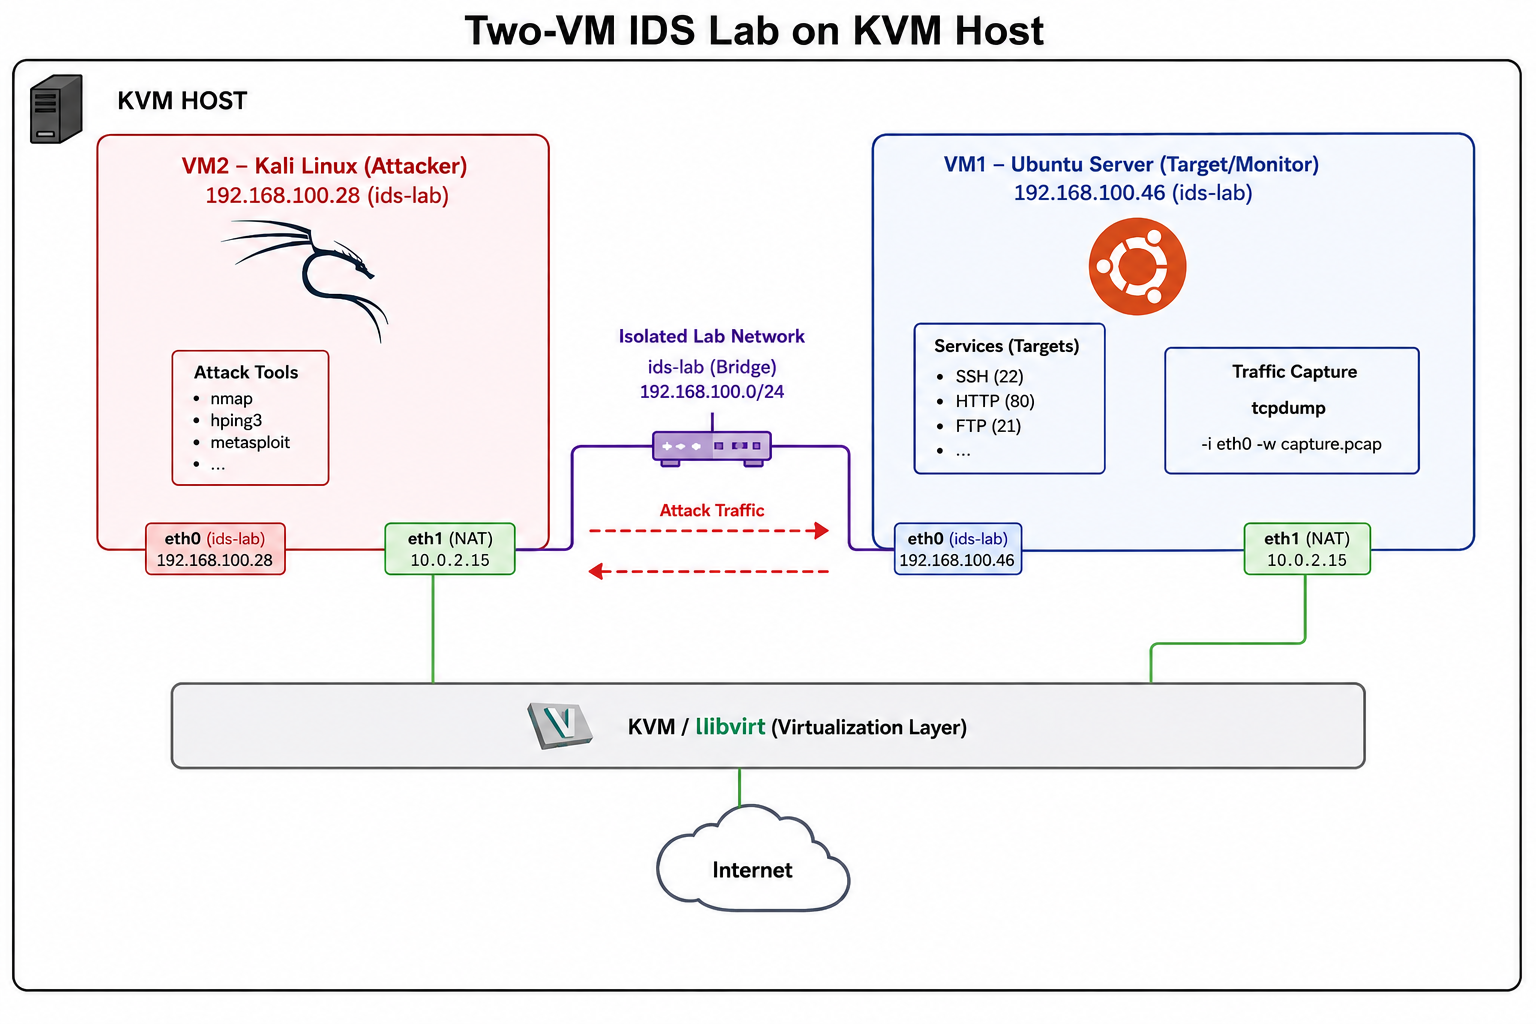
\includegraphics[width=0.9\textwidth]{figures/lab_topology.png}%
  }{%
    \fbox{\parbox{0.85\textwidth}{\centering\vspace{1.0cm}
    \texttt{[Figure: lab\_topology.png]}\\[4pt]
    \small Two-VM lab on the KVM host. VM2 (Kali, 192.168.100.28) launches
    attacks across the isolated \texttt{ids-lab} bridge toward VM1
    (Ubuntu Server, 192.168.100.46), which runs the target services and
    captures traffic with \texttt{tcpdump}. A second NAT interface on each VM
    provides internet access and carries no experimental traffic.
    \vspace{1.0cm}}}%
  }
  \caption{Realised two-machine laboratory on the KVM host.}
  \label{fig:lab_topology}
\end{figure}

We first ensured the system was set up to a known to a desired state before we moved to doing any scanning: that the two machines could reach one another across the segregated network, that the target services on VM1 returned requests, and that a traffic capture performed on VM1 with an attack against another machine (VM2) successfully captured the attack. With the environment established we were then ready for the rest of work!

% ─────────────────────────────────────────────────────────────
\section{Dataset Preparation}
\label{sec:results_dataset}

The detector is trained using \cite{sharafaldin2018cicids} the reasons of which are detailed in Section \ref{sec:conception_dataset}: it contains realistic traffic, it contains attack types that we want to experiment within the lab and the features file is also extracted using CICFlowMeter which the same as the tool which it is used live, thus, we maintain consistency of feature presentation. For the traffic captured within five days, we keep two days for training purposes; for the rest two days, we select six files for training purposes covering benign traffic, brute-force, Denial of service (DoS), web attack, Port Scanning and Distributed denial of service (DDoS); those other days, like “Infiltration” and “Botnet”, are excluded as demonstrated in Table \ref{tab:dataset_days}.

\subsection{Cleaning the raw feature files}
\label{sec:results_cleaning}

The released feature files are not of immediately use, and dealing with them threw up three specific issues that it would be good to record, since these also constitute work: 1. Column names: many rows containing column headers have leading spaces  for example “ Flow Duration” rather than “Flow Duration” ; the very first thing we have to do, therefore, is to trim white space from all column names, lest anything is refered to them by the wrong name. 2. Invalid numeric values: several of the features generated by CICFlowMeter are of the type rate bytes or packets per second and when the time duration of the flow being considered goes to 0, they write down an infinite value.

These infinite values make, however, it impossible to train any form of machine learning model, so we have opted to substitute them (positive and negative, individually) by a special missing value indicator and to remove any row with an infinity value. 3. Damaged label information for web-attack file: some attack names present in the original web-attack file have some illegal characters generated from some faulty encoding conversion, we clean-up such issue so that any row in the web-attack-traffic has a unique label. Furthermore (this one being a minor one compared to the others) they show a header row that is duplicated; we remove it at the same time in order to avoid an erroneous double counting of a features value.

Table~\ref{tab:cleaning_audit} records what each of these steps costs in flows, so that the size of the prepared dataset can be traced back to the released files.

\begin{table}[H]
  \centering
  \caption{Effect of each cleaning step on the number of flows.}
  \label{tab:cleaning_audit}
  \renewcommand{\arraystretch}{1.3}
  \begin{tabularx}{\textwidth}{Xrr}
    \toprule
    \textbf{Step} & \textbf{Flows removed} & \textbf{Flows remaining} \\
    \midrule
    Loaded from the eight released capture files & -       & 2,830,743 \\
    Rows holding an infinite or missing value    & 2,867   & 2,827,876 \\
    Exact duplicate flow records                 & 255,236 & 2,572,640 \\
    Flows labelled Infiltration or Bot           & 1,984   & 2,570,656 \\
    \midrule
    \textbf{Retained for modelling}              &         & \textbf{2,570,656} \\
    \bottomrule
  \end{tabularx}
\end{table}

Of the flows that remain, 16.5\% carry an attack label. Removing the duplicates is the step that matters most for the credibility of everything that follows: identical flow records falling on both sides of the train/test split would let the model be scored on rows it had already seen while training, which inflates every number reported later in this chapter.

\subsection{Label distribution and the imbalance problem}
\label{sec:results_imbalance}

The data, once combined, and washed clean, presents the class imbalance we suspected would result from our data collection process, from Chapter~\ref{chap:conception} that benign flows are largely in the majority, and combined across all attack types, we only have minority classes. Figure~\ref{fig:label_dist} demonstrates this. This is a typical class balance scenario where we will see that accuracy could trick the system, where a model that guesses every packet as benign still performs well for accuracy, yet detects nothing, which is why accuracy is presented in combination with recall, precision and F1, below.

\begin{figure}[H]
  \centering
  \IfFileExists{figures/label_distribution.png}{%
    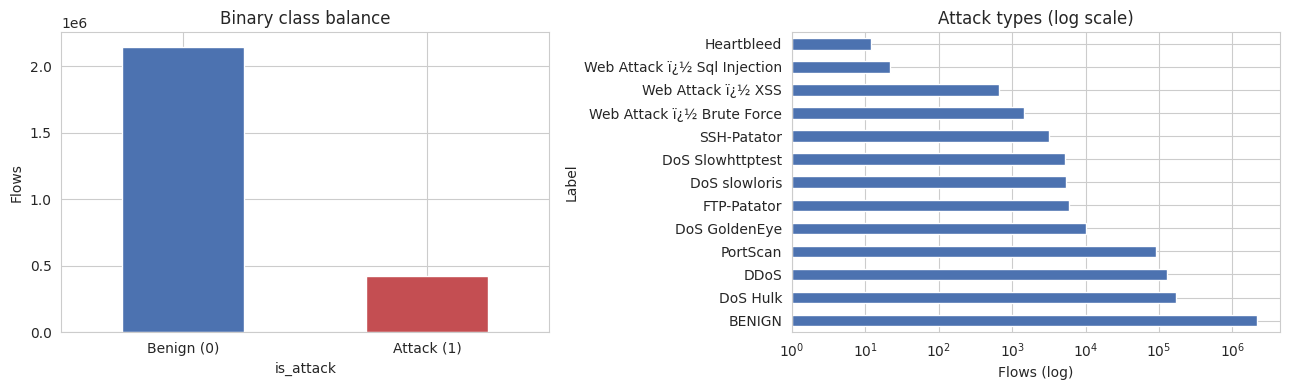
\includegraphics[width=\textwidth]{figures/label_distribution.png}%
  }{%
    \fbox{\parbox{1\textwidth}{\centering\vspace{4.0cm}
    \texttt{[Figure: label\_distribution.png]}\\[8pt]
    \small Class distribution across the six retained CICIDS-2017 files.
    Benign traffic forms the large majority; the attack classes
    (DoS, DDoS, PortScan, brute force, web attacks) form the minority,
    motivating imbalance-aware metrics and class weighting.
    \vspace{4.0cm}}}%
  }
  \caption{Distribution of benign and attack flows in the prepared dataset.}
  \label{fig:label_dist}
\end{figure}

From a different perspective, two different features offer the same view of the data. Figure~\ref{fig:eda_hist} shows the benign and attack distribution overlayed for flow duration and forward packet count. The attack distribution mostly overlies the benign distribution across most of the range, and the two separate only in the tails. This indicates we will need a learned model as this would require a very high sensitivity threshold to be manually defined and still not perform well. The signal is likely in the interactions of a set of features, not contained in a single feature, which is the goal for the candidates in Section~\ref{sec:results_models}.

\begin{figure}[H]
  \centering
  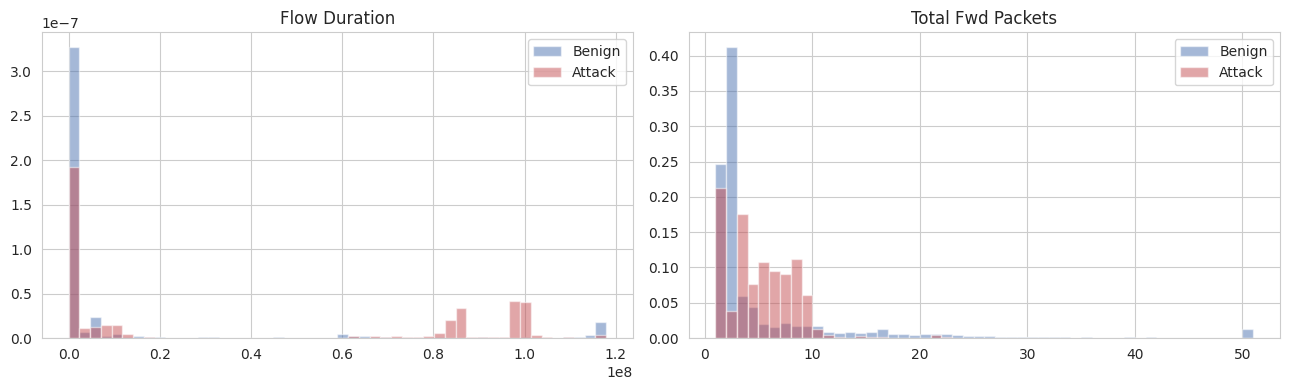
\includegraphics[width=\textwidth]{figures/eda_feature_histograms.png}
  \caption{Benign against attack distributions for two example features. Values are clipped at the 99th percentile and drawn as densities, so that the two very unequal class sizes stay comparable.}
  \label{fig:eda_hist}
\end{figure}

% ─────────────────────────────────────────────────────────────
\section{Feature Engineering and Selection}
\label{sec:results_features}

CICFlowMeter represents each flow using 79 features. Features can be grouped into several families of features: flow identifiers \& destination port, number of forward and backward packets and bytes, packet lengths statistics, inter-arrival time for flow, backward and forward direction, number of various tcp flags in flow, flow rates, connection-window and sub-flow characteristics. For instance, Flow Duration is feature counting the length of a connection, Total Fwd Packets number of packets moving toward forward direction, SYN Flag Count number of syn flags contained in the flow, or Flow Bytes/s represents amount of bytes carried in each direction within one second. Full list of CICFlowMeter's features is attached in Appendix~\ref{app:features} with brief definitions.

In addition we add 3 more engineered features those are features derived by explicitly forming a ratio that models a relationship that we either want the model to recognize easily or the model would likely fail to generalize properly, if we only rely on it inferring: ratio of forward to backward packets, ratio of forward to backward byte counts, and average forward packet size. They effectively codify a directional flow asymmetry to one value, something characteristic for a one sided flood as opposed to a balanced conversation.
 


Not all features have informativeness, for example, a few show almost equal values throughout the data and thus do not assist in discrimination. These features are subsequently removed through the use of a variance filter. This variance filter removed a total of eight columns, which contained equal values for each flow in the prepared dataset, namely the six bulk-transfer counters, backward PSH flag count and backward URG flag count.

The second layer of reduction is not the result of missing data but rather indicative of excessive redundancy. There appears to be (almost) duplicate values across the range of features, either because these features represent the same values under alternative names or because the features are simply a (non-unique) function of each other. Fig~\ref{fig:corr_heatmap} demonstrates the block structure of this correlation matrix.
When two variables are highly correlated (> 0.95) in the training split, one is discarded, which leads to the removal of a further 23 columns from the data set; see appendix~\ref{app:feat_dropped} for the names and duplicates of all removed features.
Two of the discarded features are particularly relevant to the next sections and are included here; the SYN flag count is discarded as the value is numerically the same as that of the forward PSH flag count for this data set, which means there is no SYN counter as an input to the deployed detector, and similarly for the ratio of the mean forward packet size (out of the three ratios that are engineered). Note that only two of the three ratios are used in the models. It can be seen from table~\ref{tab:feature_reduction} that the number of features is reduced stage by stage, ending at the 49 features that are used by the models, which the deep models then standardise before use.

\begin{table}[H]
  \centering
  \caption{Feature count at each stage of preparation.}
  \label{tab:feature_reduction}
  \renewcommand{\arraystretch}{1.3}
  \begin{tabularx}{\textwidth}{Xr}
    \toprule
    \textbf{Stage} & \textbf{Features} \\
    \midrule
    Numeric features in the released CSV files                      & 78 \\
    After removing the duplicated \texttt{Fwd Header Length} column & 77 \\
    After adding the three engineered ratios                        & 80 \\
    After the variance filter, (-8) constant columns                & 72 \\
    After the correlation filter, (-23) redundant columns           & \textbf{49} \\
    \bottomrule
  \end{tabularx}
\end{table}

\begin{figure}[H]
  \centering
  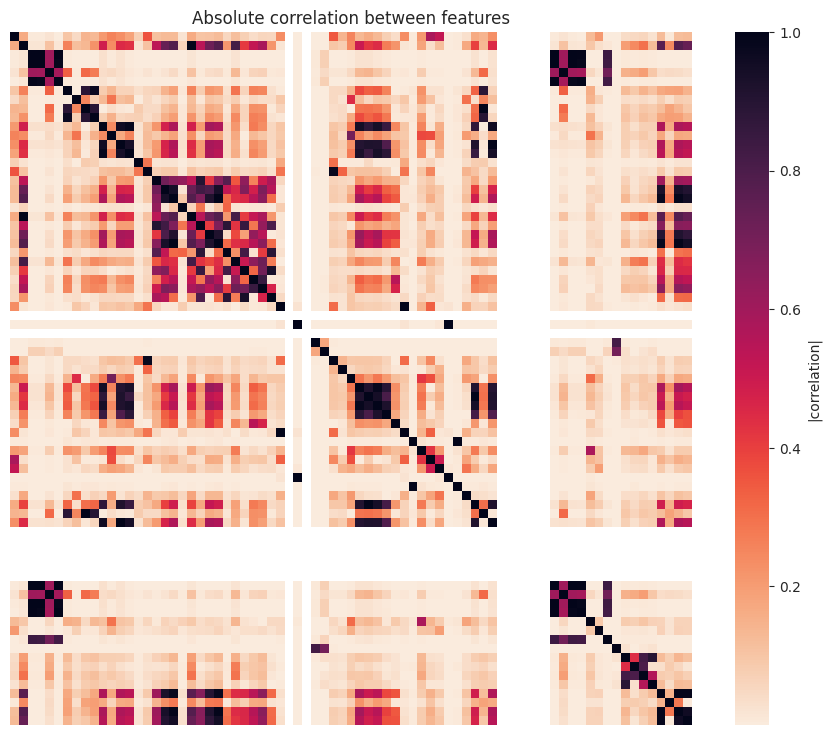
\includegraphics[width=0.82\textwidth]{figures/correlation_heatmap.png}
  \caption{Absolute correlation between the candidate features, on a sample of 300,000 flows. Axis labels are deliberately omitted; what matters is the block structure, each dark square being a group of features carrying nearly the same information.}
  \label{fig:corr_heatmap}
\end{figure} 


These 49 features are preserved along with their order alongside the model. It is important that the features given to the model are exactly those used during training.

The last detail to note is what is called order of operation. The details seem to be often glossed over but: all preparatory steps that learn anything from data; namely applying the variance filter, feature scaling as required for deep models, and resampling for balancing classes of training data; are determined on the training set only. Applying these steps prior to splitting the training/testing data would let information flow from the test set into the training set and hence cause over-estimation of results.

% ─────────────────────────────────────────────────────────────
\section{Model Development and Comparison}
\label{sec:results_models}


Chapter~\ref{chap:conception} had required to train a set of candidate models instead of a single one, in order for the data to decide in the classical or deep learning dilemma. It was eventually decided to train three models: a Random Forest (classical method), a Convolutional Neural Networks (CNN) and a Long Short-Term Memory network (LSTM). These last two are deep learning models, the LSTM being more suitable for sequential data, which should theoretically be optimal when attackers embed data into the order of the packets. These training runs were performed off the lab machines, on a Google Colab GPU, to make a clear separation of concern, as explained in Section~\ref{sec:conception_offline}.
A single split of the data was performed before any training, shared by all three models, to ensure a fair comparison. The split was selected as detailed in table~\ref{tab:protocol}. The three models were trained on the same stratified subsample of the training data so that the comparison would not take too long on a free GPU.
After the training, models were tested on a validation sample obtained from the same data, not the test set.
The test set was only used in section~\ref{sec:results_benchmark} to make one assessment. Using the test set to decide which model was best would have caused a bias, which would have the effect of adding performance to the models in a meaningless way. Values for each model are summarized in table~\ref{tab:hyperparams}.

\begin{table}[H]
  \centering
  \caption{Data partitions used for training, model selection and final evaluation.}
  \label{tab:protocol}
  \renewcommand{\arraystretch}{1.3}
  \begin{tabularx}{\textwidth}{Xrl}
    \toprule
    \textbf{Partition} & \textbf{Flows} & \textbf{Used for} \\
    \midrule
    Training set, 80\%              & 2,056,524 & everything fitted from data \\
    \quad bake-off subsample        & 370,174   & training the three candidates \\
    \quad validation split          & 205,653   & choosing the winner and the threshold \\
    Test set, 20\%, held back       & 514,132   & one final evaluation of the winner \\
    \bottomrule
  \end{tabularx}
\end{table}

\begin{table}[H]
  \centering
  \caption{Configuration of the three candidate models. Every run uses seed 42.}
  \label{tab:hyperparams}
  \renewcommand{\arraystretch}{1.3}
  \begin{tabularx}{\textwidth}{lX}
    \toprule
    \textbf{Model} & \textbf{Configuration} \\
    \midrule
    Random Forest (bake-off) & 100 trees, unlimited depth, square root of the feature count considered per split, balanced class weights, unscaled inputs \\
    Random Forest (deployed) & 200 trees, otherwise identical, retrained on the full training set \\
    CNN  & two one-dimensional convolutions, 1 to 32 and 32 to 64 channels with kernel size 3, ReLU and batch normalisation, adaptive max pooling, dense layer of 64 units, dropout 0.3 \\
    LSTM & one LSTM layer of 64 hidden units reading the feature vector as the sequence dimension, dense layer of 32 units, dropout 0.3 \\
    Both deep models & Adam at learning rate $10^{-3}$, batch size 1024, at most 15 epochs, early stopping with patience 3, class-weighted cross-entropy, standardised inputs \\
    \bottomrule
  \end{tabularx}
\end{table}

The comparison on the validation split is given in Table~\ref{tab:model_comparison}. It is the unexpected answer Chapter~\ref{chap:conception} teased at: Random Forest not only keeps up with the two deep models, but it outperformes both on all interesting measures; additionally it is also far less expensive both in training and execution.

\begin{table}[H]
  \centering
  \caption{Candidate model performance on the validation split of CICIDS-2017.}
  \label{tab:model_comparison}
  \renewcommand{\arraystretch}{1.3}
  \begin{tabularx}{\textwidth}{Xccccc}
    \toprule
    \textbf{Model} & \textbf{Precision} & \textbf{Recall} & \textbf{F1} & \textbf{ROC-AUC} & \textbf{PR-AUC} \\
    \midrule
    Random Forest & \textbf{0.9973} & \textbf{0.9961} & \textbf{0.9967} & \textbf{0.9998} & \textbf{0.9986} \\
    CNN           & 0.8713 & 0.9931 & 0.9282 & 0.9986 & 0.9930 \\
    LSTM          & 0.8645 & 0.9889 & 0.9225 & 0.9979 & 0.9903 \\
    \bottomrule
  \end{tabularx}
\end{table}


Figure~\ref{fig:model_bars} visualizes the above three rows in a diagram and the confusion matrices in Figure~\ref{fig:cm_validation} show what is lost between those summary metrics. Expressed as a precision of 0.87 the gap in false alarms looks modest, but in absolute terms it is large, and the main effect is the additional burden on an analyst's workflows. For 205,653 flows during validation, all three models detected virtually all the attack flows, with a recall never falling below 0.988.
The difference is in the benign flows, where the random forest generated 93 false alarms, but the CNN generated 4,975 and the LSTM model 5,253, more than fifty times as many.
In terms of detection, this is not significant, but in terms of workload and the tradeoffs in the cost to the analyst, it is. In this context, we can also revisit the situation raised in Section~\ref{sec:ids_commercial} with respect to noisy detectors.

\begin{figure}[H]
  \centering
  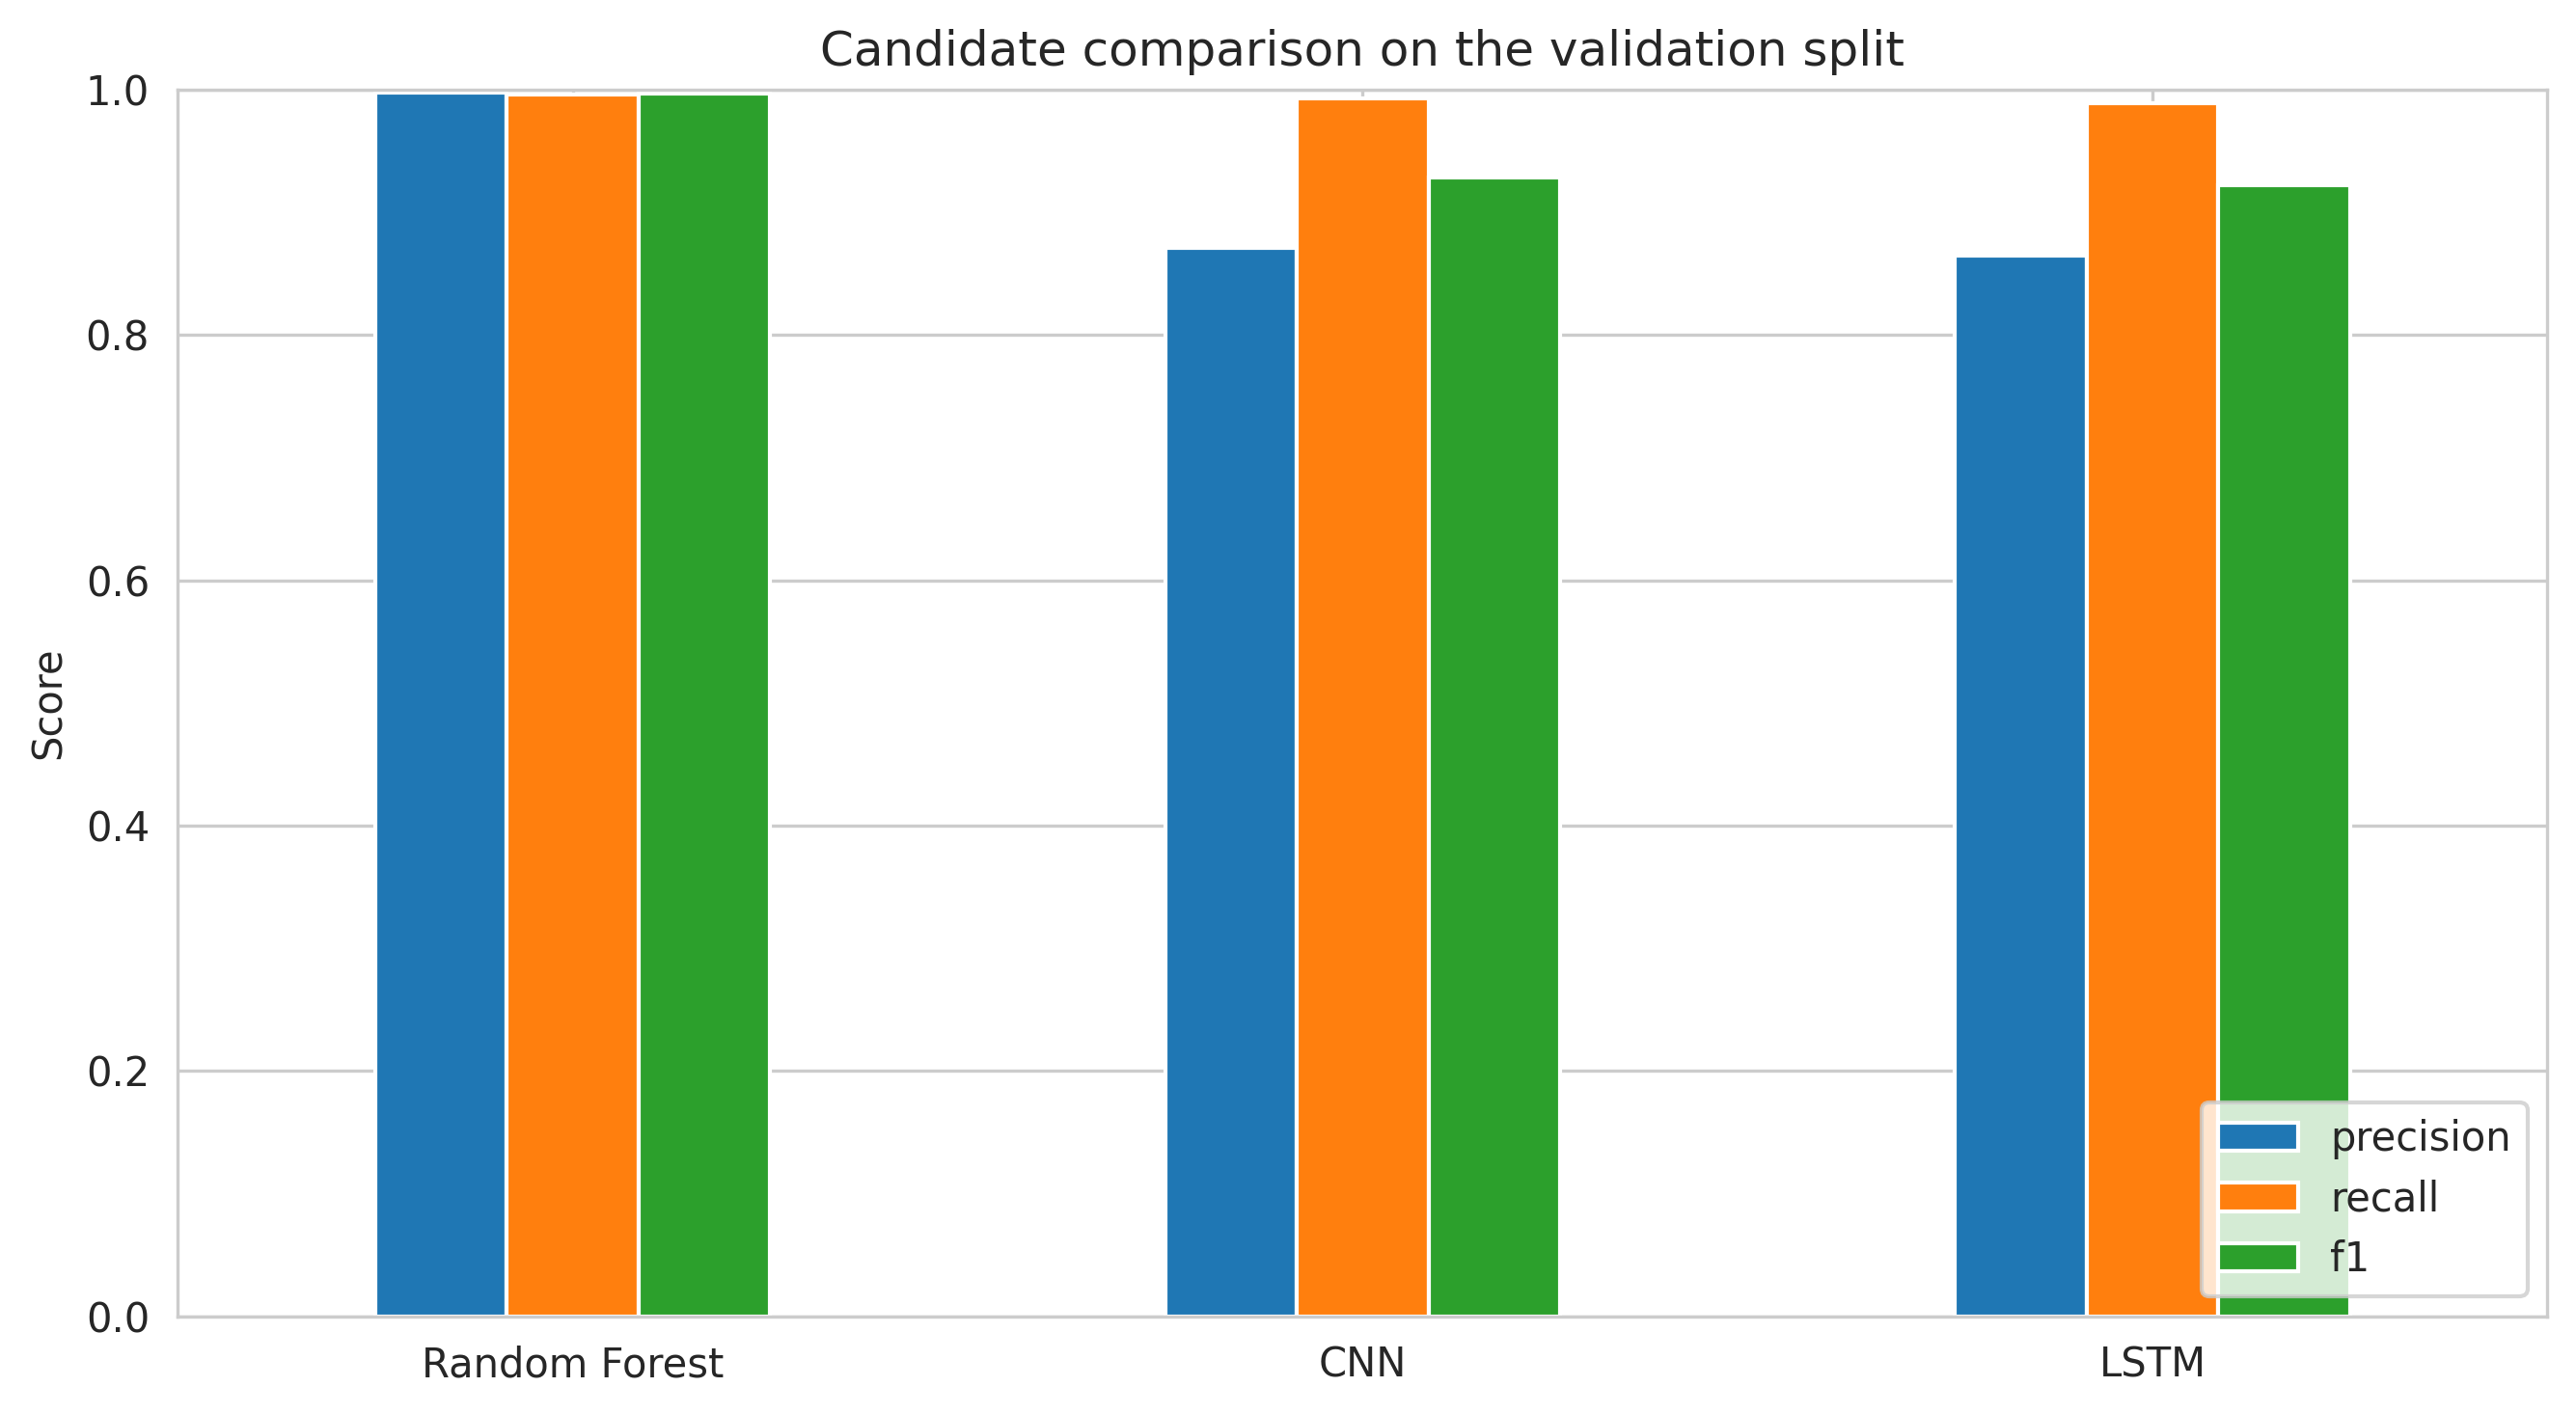
\includegraphics[width=0.85\textwidth]{figures/model_comparison_bars.png}
  \caption{Precision, recall and F1 of the three candidates on the validation split.}
  \label{fig:model_bars}
\end{figure}

\begin{figure}[H]
  \centering
  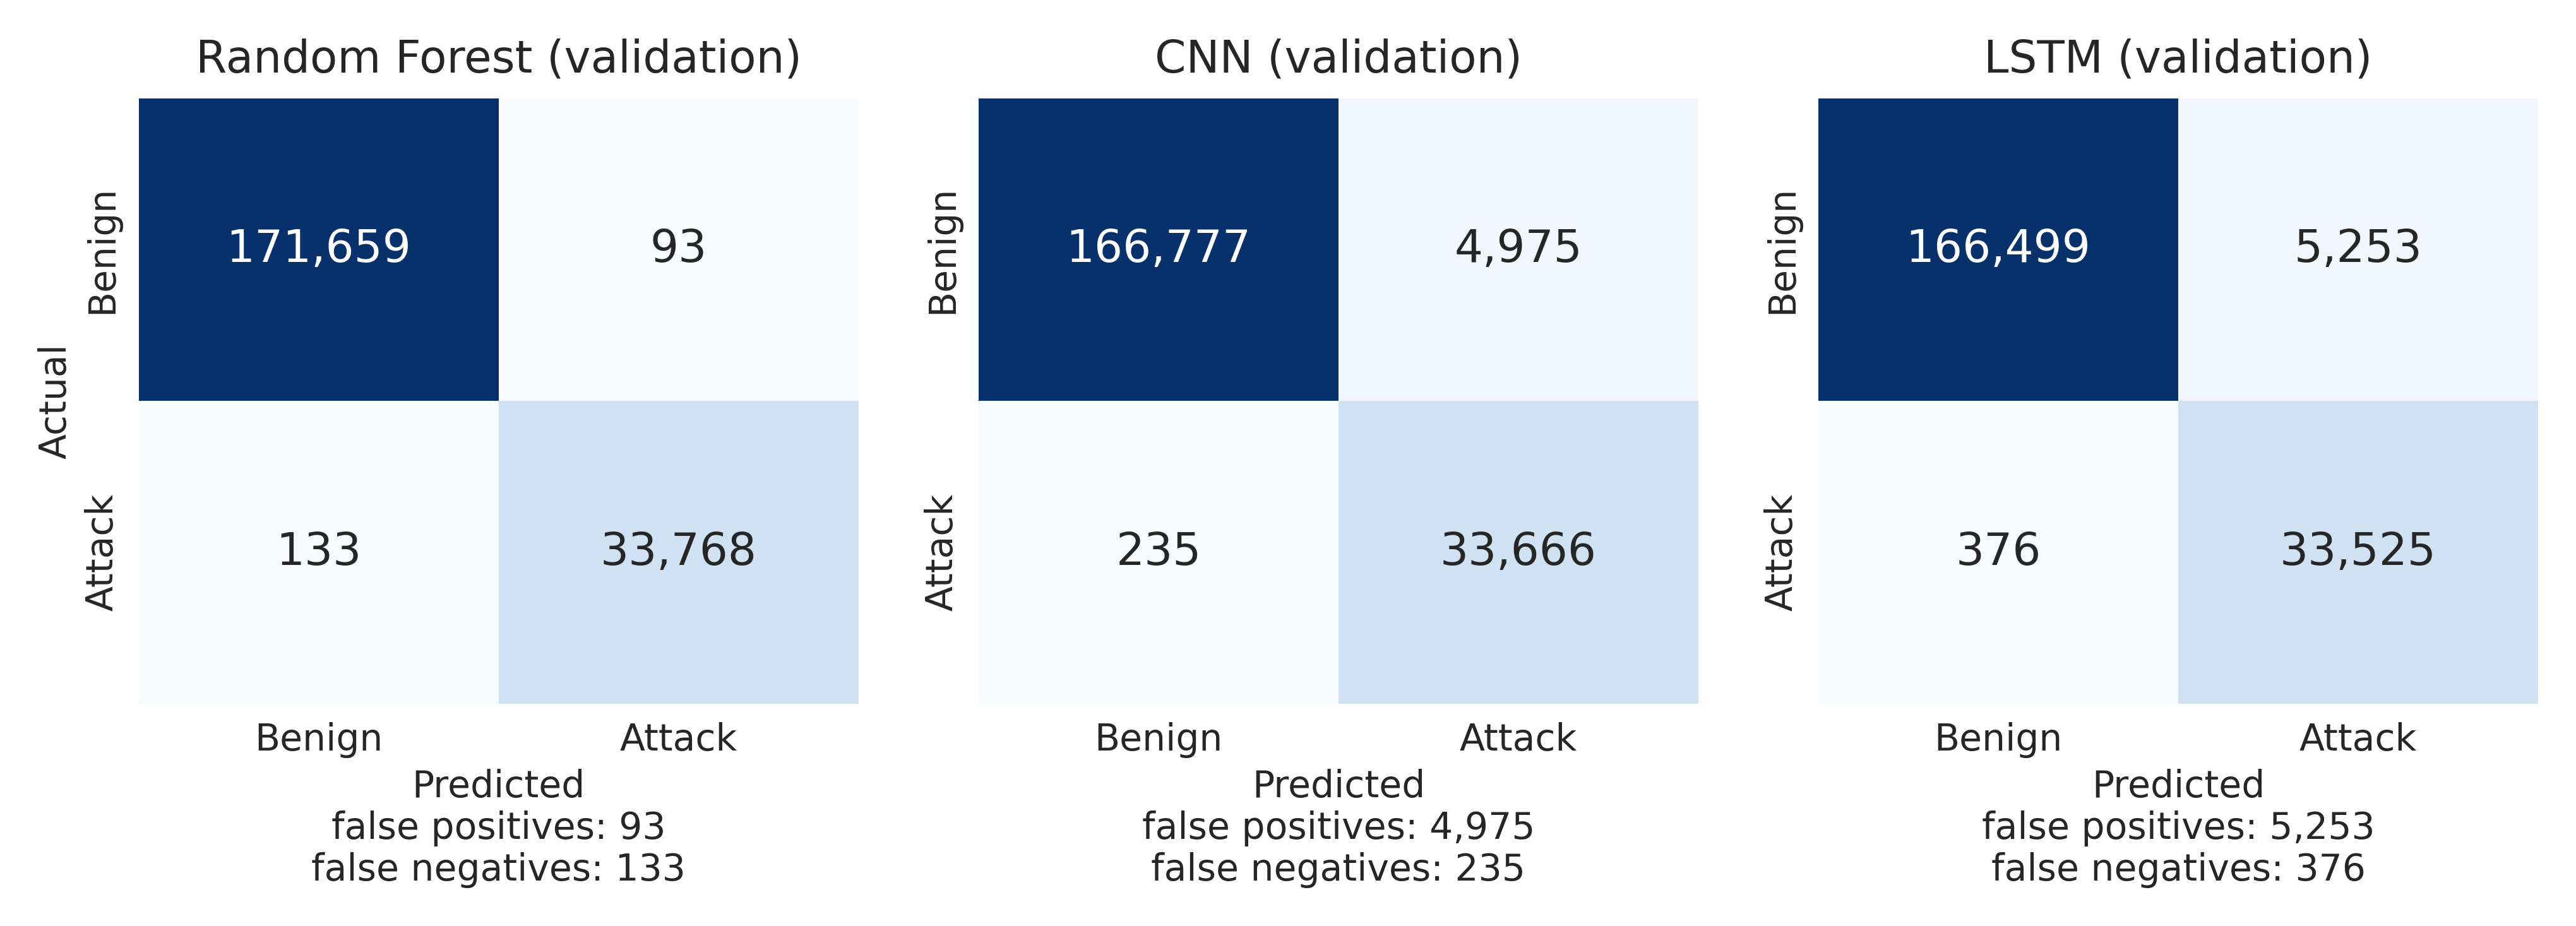
\includegraphics[width=\textwidth]{figures/cm_validation_three_models.png}
  \caption{Validation confusion matrices of the three candidates over the same 205,653 flows. The models are separated by their false-positive counts, not by their ability to catch attacks.}
  \label{fig:cm_validation}
\end{figure}

Perhaps this should not be as surprising as it seems, and this is what we would expect from Chapter~\ref{chap:ai}. For strong, already-reduced tabular features like these, it is very difficult to do better than the tree-ensemble models: they don’t require feature scaling, aren’t hurt by features with completely disparate scales, and don’t have the large, complex, precisely-tuned budgets required by deep learning models just to get to baseline. The deep models in our sample performed adequately overall; they hit our recall objective at the expense of additional false positives, and were far more computationally expensive to train ( and to operate: they consume more memory/CPU for inference). 
A detector we’re trying to run on a reasonably small machine could do better as a result of deploying a Random Forest: not only did it perform better but the overhead is low, and engineering costs low too. 
That doesn’t mean anything profound about deep learning models in general; only that that’s what we found for this job, on this data, which was the intention of Chapter~\ref{chap:conception}.

Using our chosen random forest, we tuned the decision threshold to values other than one half. Since the penalty for failing to detect an attack is different than the penalty for claiming there was an attack there was, a better model can be made by tuning threshold; our tuned threshold yielded the highest F1 on the validation set. The model we picked can class something like forty five thousand of these per second, which is the throughput necessary for real-time operation; it will crop up in the Discussion again.

% ─────────────────────────────────────────────────────────────
\section{Benchmark Evaluation}
\label{sec:results_benchmark}
 
On the held-out CICIDS-2017 data the winning Random Forest performs near flawlessly on the unseen data: F1 score $\approx 0.997$, ROC-AUC $\approx 0.9998$. Figure~\ref{fig:rf_confusion} shows the confusion matrix for this winning model, where almost every flow lands on the correct diagonal. In isolation, this would be more reason for skepticism than celebration, as a victory on a benchmark makes claims more about the benchmark itself than about real-world data.

\begin{figure}[H]
  \centering
  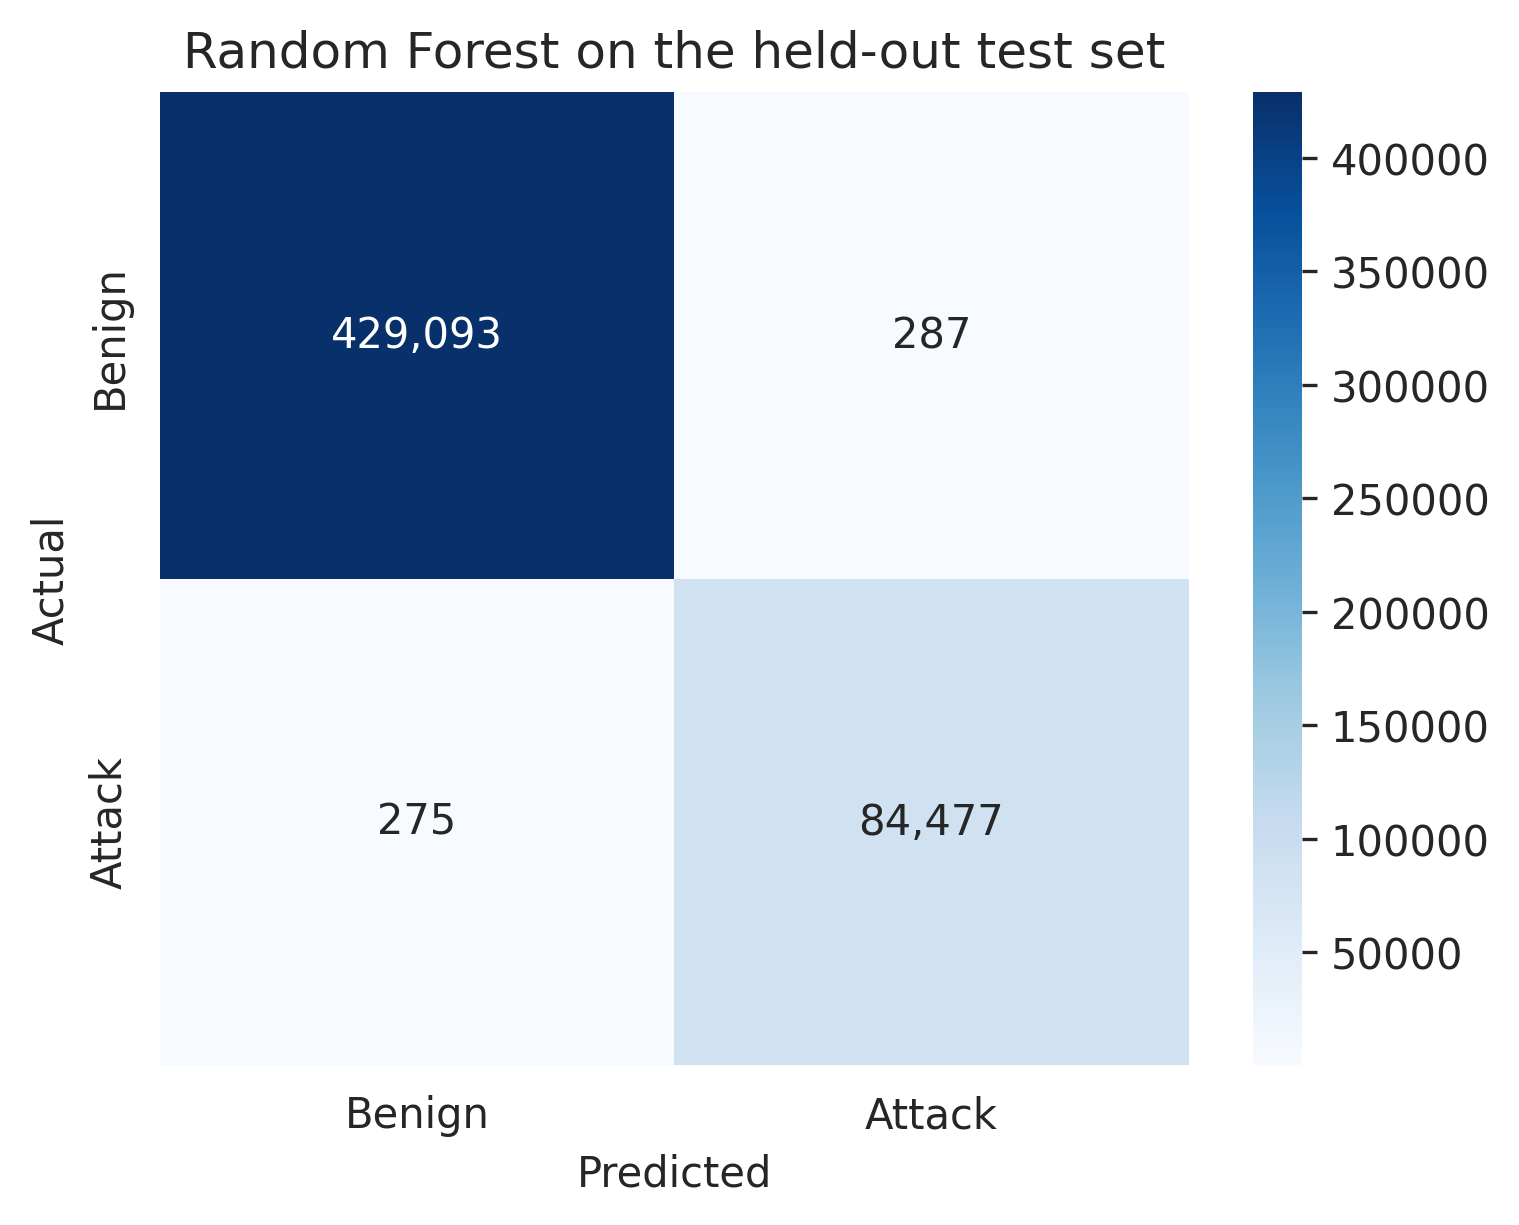
\includegraphics[width=0.62\textwidth]{figures/cm_rf_test.png}
  \caption{Confusion matrix of the deployed Random Forest on the held-out CICIDS-2017 test set.}
  \label{fig:rf_confusion}
\end{figure}

Of the total 514,132 test flows in total, out of which 287 benign flows are detected as attacks and 275 attacks are not detected when compared to 429,380 benign flows and 84,752 attacks. These four inferences are forming precision of 0.9966 and recall of 0.9968 in absolute values.


Since our dataset is imbalanced the precision-recall curve provides better insight than the ROC curve in our case: in a dataset dominated by normal traffic an ROC curve can show satisfactory results merely by the sheer number of correctly predicted negative values. The view on the precision-recall curve represents how accurately our attacks are being caught. Figure~\ref{fig:rf_pr} displays the PR curve of our finalized model over the test set, which identifies two points of operation-the default decision threshold of one half and the threshold we picked on the validation dataset (described in section~\ref{sec:results_models}). The PR curve also illustrates the tuning of decision threshold, yielding a slight decrease in one aspect when we chose to increase the other.
 
\begin{figure}[H]
  \centering
  \IfFileExists{figures/rf_pr_curve.png}{%
    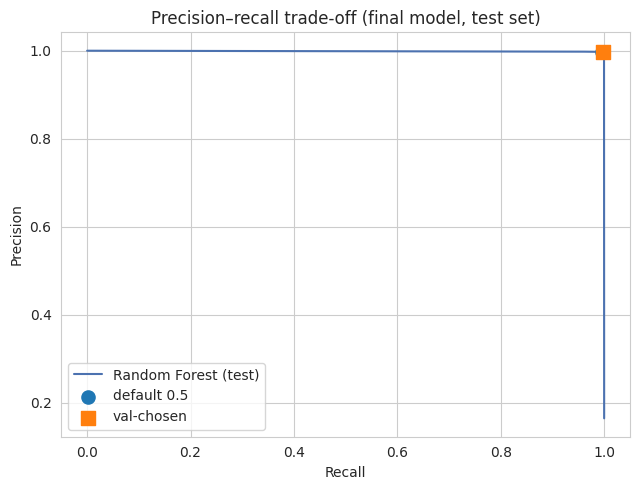
\includegraphics[width=0.7\textwidth]{figures/rf_pr_curve.png}%
  }{%
    \fbox{\parbox{0.85\textwidth}{\centering\vspace{1.0cm}
    \texttt{[Figure: rf\_pr\_curve.png]}\\[4pt]
    \small Precision--recall trade-off of the final Random Forest on the test
    set, with the default (0.5) and validation-chosen operating points marked.
    Exported from the training notebook.
    \vspace{1.0cm}}}%
  }
  \caption{Precision-recall trade off of the selected model, with both operating points.}
  \label{fig:rf_pr}
\end{figure}

Table~\ref{tab:operating_points} quantifies the two points. Changing the threshold from the default of 0.5 to the validation-split-selected threshold of 0.340 increases recall from 0.9968 to 0.9987; this recovers about 160 more attacks out of the 84,752, at a cost of three ten-thousandths of precision. This may be an acceptable tradeoff for a detection system. Both rows are shown because the threshold is an operating choice of the system operators rather than a property of the model itself.


\begin{table}[H]
  \centering
  \caption{Test-set performance of the deployed model at the two operating points marked in Figure~\ref{fig:rf_pr}.}
  \label{tab:operating_points}
  \renewcommand{\arraystretch}{1.3}
  \begin{tabularx}{\textwidth}{Xccc}
    \toprule
    \textbf{Decision threshold} & \textbf{Precision} & \textbf{Recall} & \textbf{F1} \\
    \midrule
    Default, 0.500                        & 0.9966 & 0.9968 & 0.9967 \\
    Chosen on the validation split, 0.340 & 0.9963 & \textbf{0.9987} & \textbf{0.9975} \\
    \bottomrule
  \end{tabularx}
\end{table}
 

The more subtle approach is to treat it as multi-class and not as a benign vs attack issue. In this context the model detects all high volume network attacks (DoS, DDoS, Port Scan, Brute Force) with near perfect accuracy but is clearly much less effective with web based attacks, where the cross-site scripting score is lower. This is of course what we might expect, the web attacks leave little trace in the flow statistics and closely resemble ordinary traffic, unlike the high volume attacks which are very different. Its a pretty straightforward benchmark for the obvious attacks but quite difficult for the less obvious which is surely the way the results should play out (and which will form the main point of the next section).


Figure~\ref{fig:cm_multiclass} and Table~\ref{tab:per_class} show the results in more detail. The results are promising, with 9 out of the 11 classes predicted almost perfectly, but the two web-attack classes are clearly hard to distinguish. The confusion matrix shows where the problem lies: 86 of the 130 cross-site scripting flows are predicted as web brute-force, while 60 brute-force flows are wrongly predicted as scripting.
This leads to a drop in the XSS F1 score to 0.36.
But these two classes look identical at the level of flow statistics: both have a short HTTP request to the same server and port, and nothing on the flow feature vector indicates whether the payload is a script or a password guess. The matrix also shows the only appreciable confusion outside the web classes, between benign flows and portscan, with 222 benign flows predicted as portscan and 159 portscan flows predicted as benign. Again, this is no surprise, as the attack and benign flows both use a very short connection and transfer very little data.

\begin{figure}[H]
  \centering
  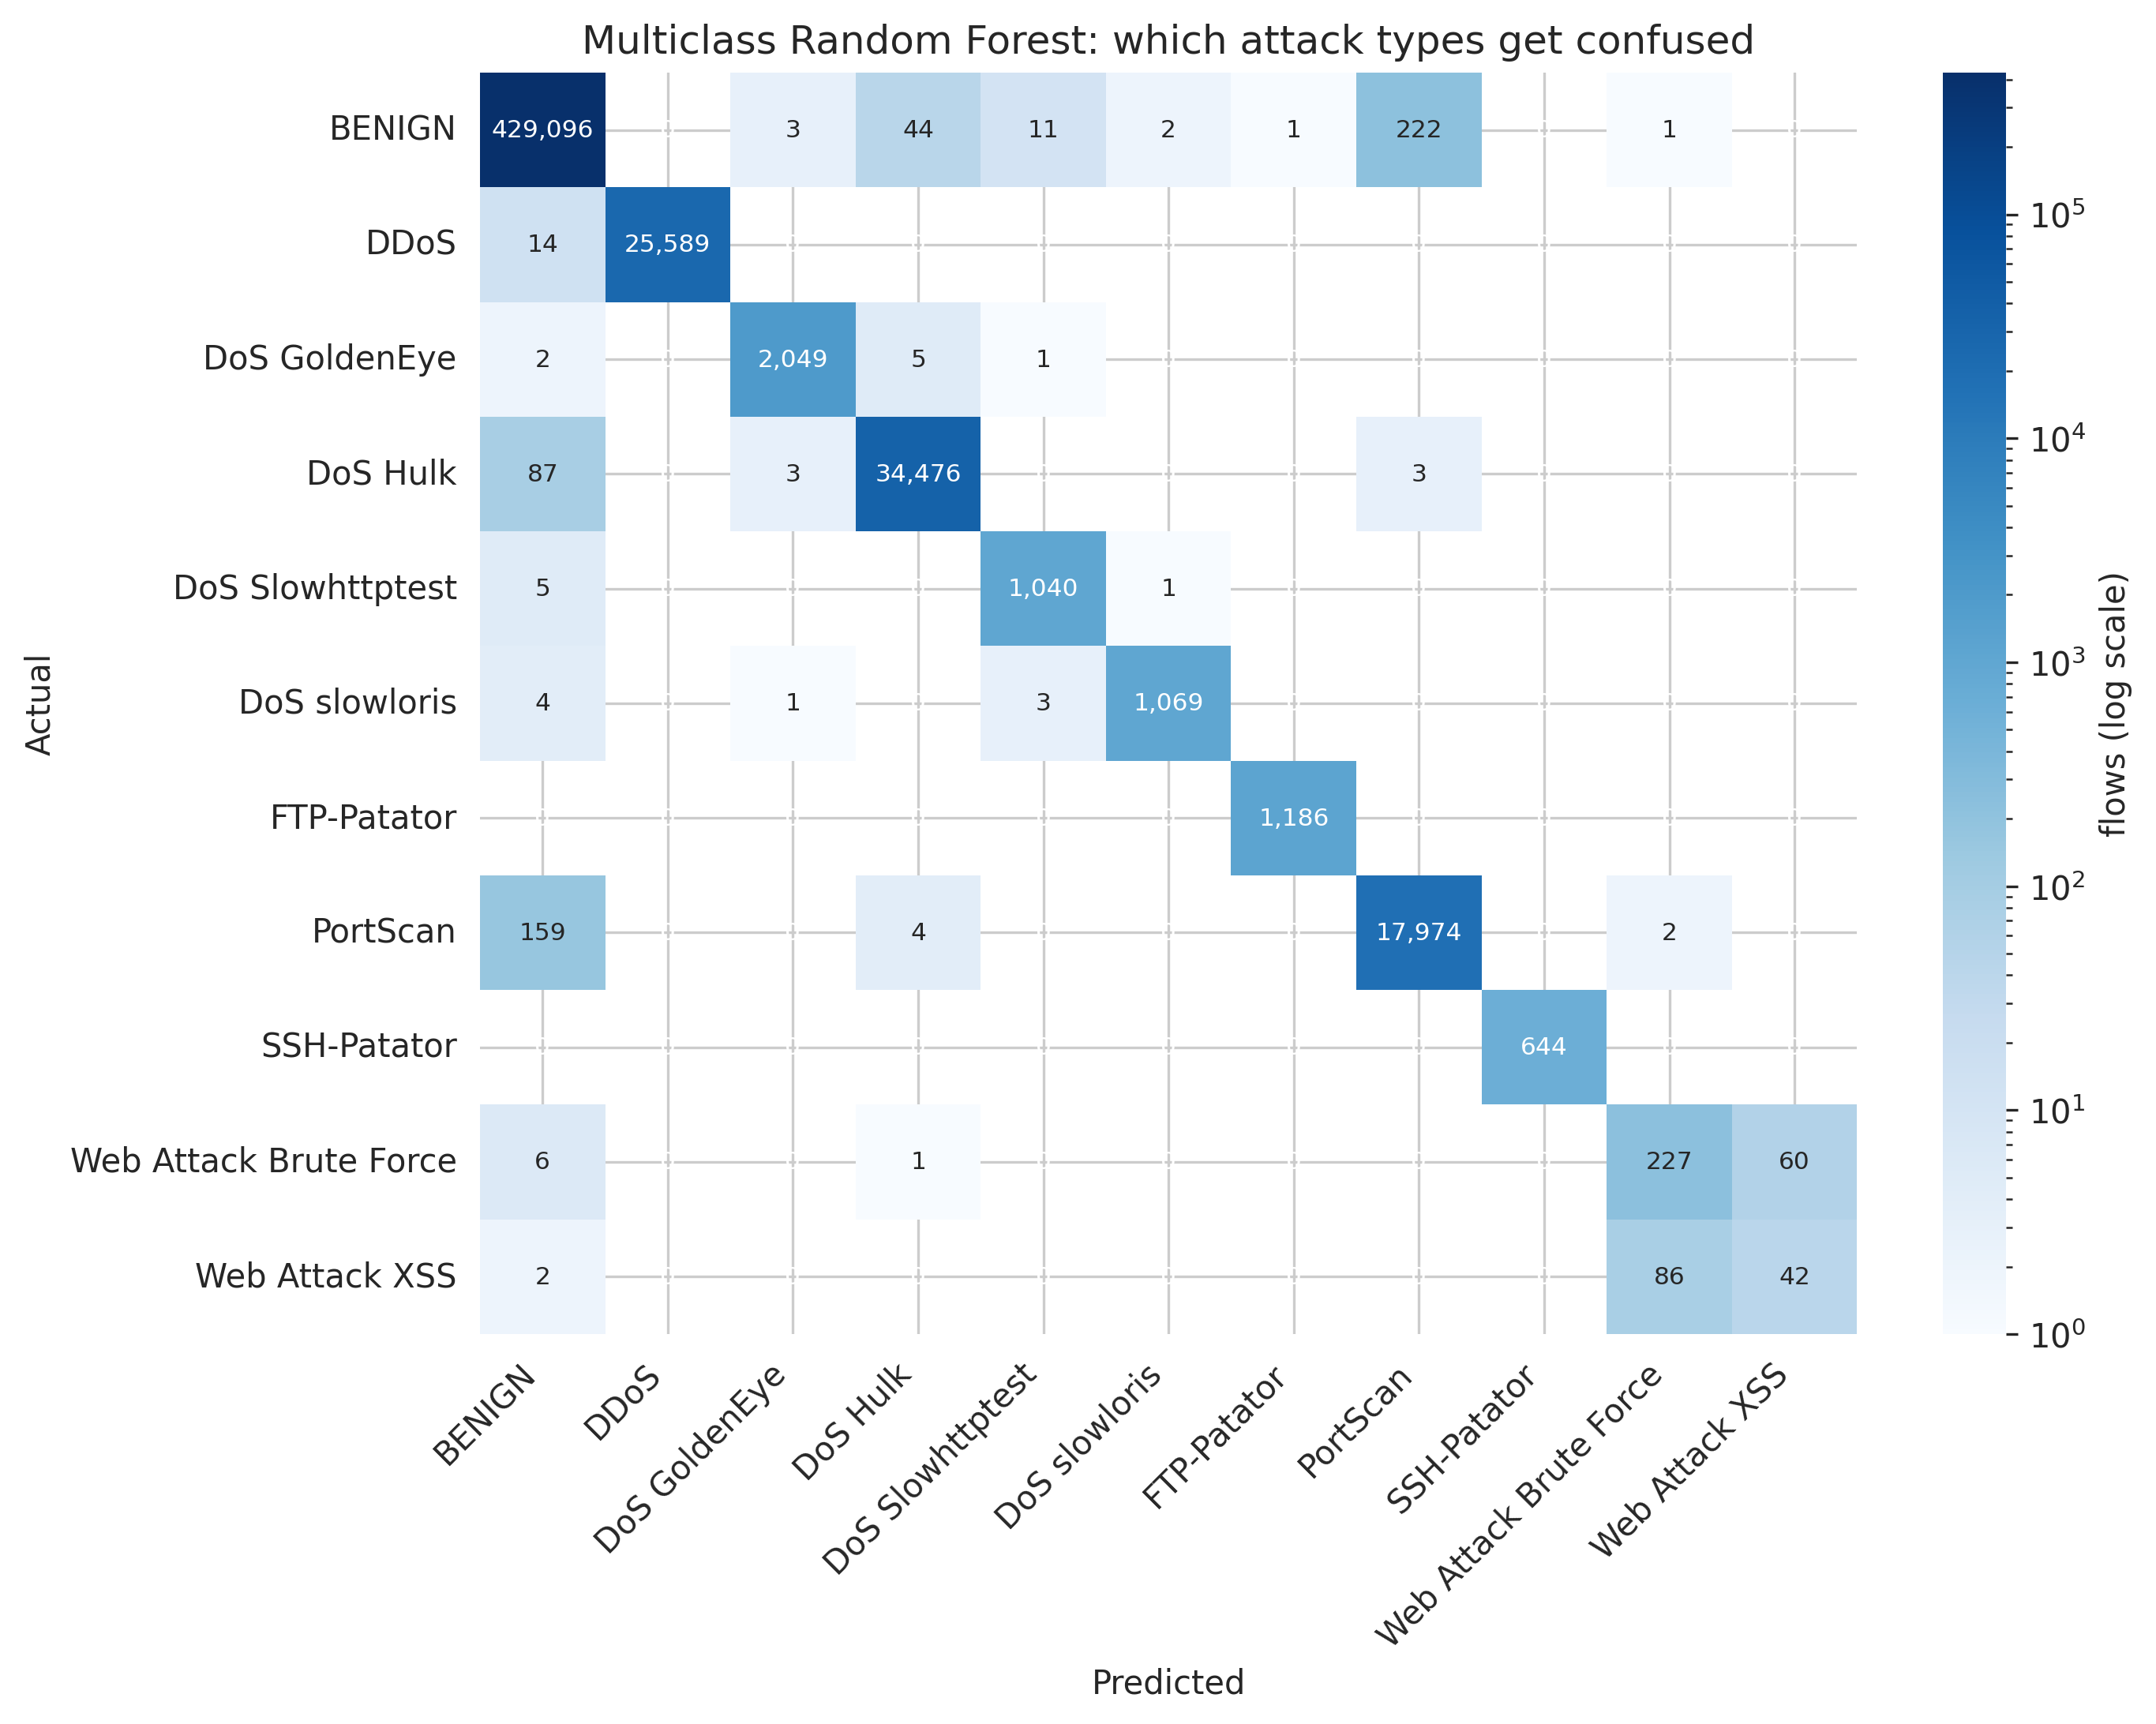
\includegraphics[width=0.86\textwidth]{figures/cm_multiclass.png}
  \caption{Confusion matrix of the multiclass Random Forest over the eleven retained attack types. The colour scale is logarithmic so that the small classes stay visible beside the benign class.}
  \label{fig:cm_multiclass}
\end{figure}

\begin{table}[H]
  \centering
  \caption{Per-class performance of the multiclass Random Forest on its held-out set.}
  \label{tab:per_class}
  \renewcommand{\arraystretch}{1.05}
  \begin{tabularx}{\textwidth}{Xcccr}
    \toprule
    \textbf{Class} & \textbf{Precision} & \textbf{Recall} & \textbf{F1} & \textbf{Flows} \\
    \midrule
    BENIGN                 & 1.00 & 1.00 & 1.00 & 429,380 \\
    DDoS                   & 1.00 & 1.00 & 1.00 & 25,603 \\
    DoS GoldenEye          & 1.00 & 1.00 & 1.00 & 2,057 \\
    DoS Hulk               & 1.00 & 1.00 & 1.00 & 34,569 \\
    DoS Slowhttptest       & 0.99 & 0.99 & 0.99 & 1,046 \\
    DoS slowloris          & 1.00 & 0.99 & 0.99 & 1,077 \\
    FTP-Patator            & 1.00 & 1.00 & 1.00 & 1,186 \\
    PortScan               & 0.99 & 0.99 & 0.99 & 18,139 \\
    SSH-Patator            & 1.00 & 1.00 & 1.00 & 644 \\
    Web Attack Brute Force & 0.72 & 0.77 & 0.74 & 294 \\
    Web Attack XSS         & 0.41 & 0.32 & 0.36 & 130 \\
    \midrule
    \textbf{Macro average} & \textbf{0.92} & \textbf{0.92} & \textbf{0.92} & 514,125 \\
    \bottomrule
  \end{tabularx}
\end{table}
 
% ─────────────────────────────────────────────────────────────
\section{Explainability with SHAP}
\label{sec:results_shap}

As I noted in the description of a verdict-only detector, this puts all the work of making sense of a score fully on the analyst. Building on the scheme described in Section~\ref{sec:conception_realtime}, we take our models outputs through a SHAP explainer which shows which features are responsible for the verdict. Instead of having one model which simply say "attack”, the explainer will show that this traffic was deemed a potential attack because it had, for example, an anomalously high number of half open connections or an anomalously short duration, thus transforming an unreadable score into something that is easily interpretable and usable by the analyst (e.g. To block traffic, escalate an incident or to confidently dismiss the incident as a false positive).

Before delving into how SHAP is used to explain the model, let's take a moment to understand the knowledge we gain from the Random Forest itself. A Random Forest algorithm will, by nature, give us an importance score for each feature, which is derived from how much the feature explains the impurity in the data as the ensemble of trees is created. Figure~\ref{fig:rf_importance} shows the top fifteen features in the deployed model, which are largely packet-size-related, the two TCP initial window sizes, and the destination port.
This explanation is quick and global, but only tells us how much the feature affects the decision, not the direction it takes or how it affects individual flows.
SHAP resolves both of these issues.


\begin{figure}[H]
  \centering
  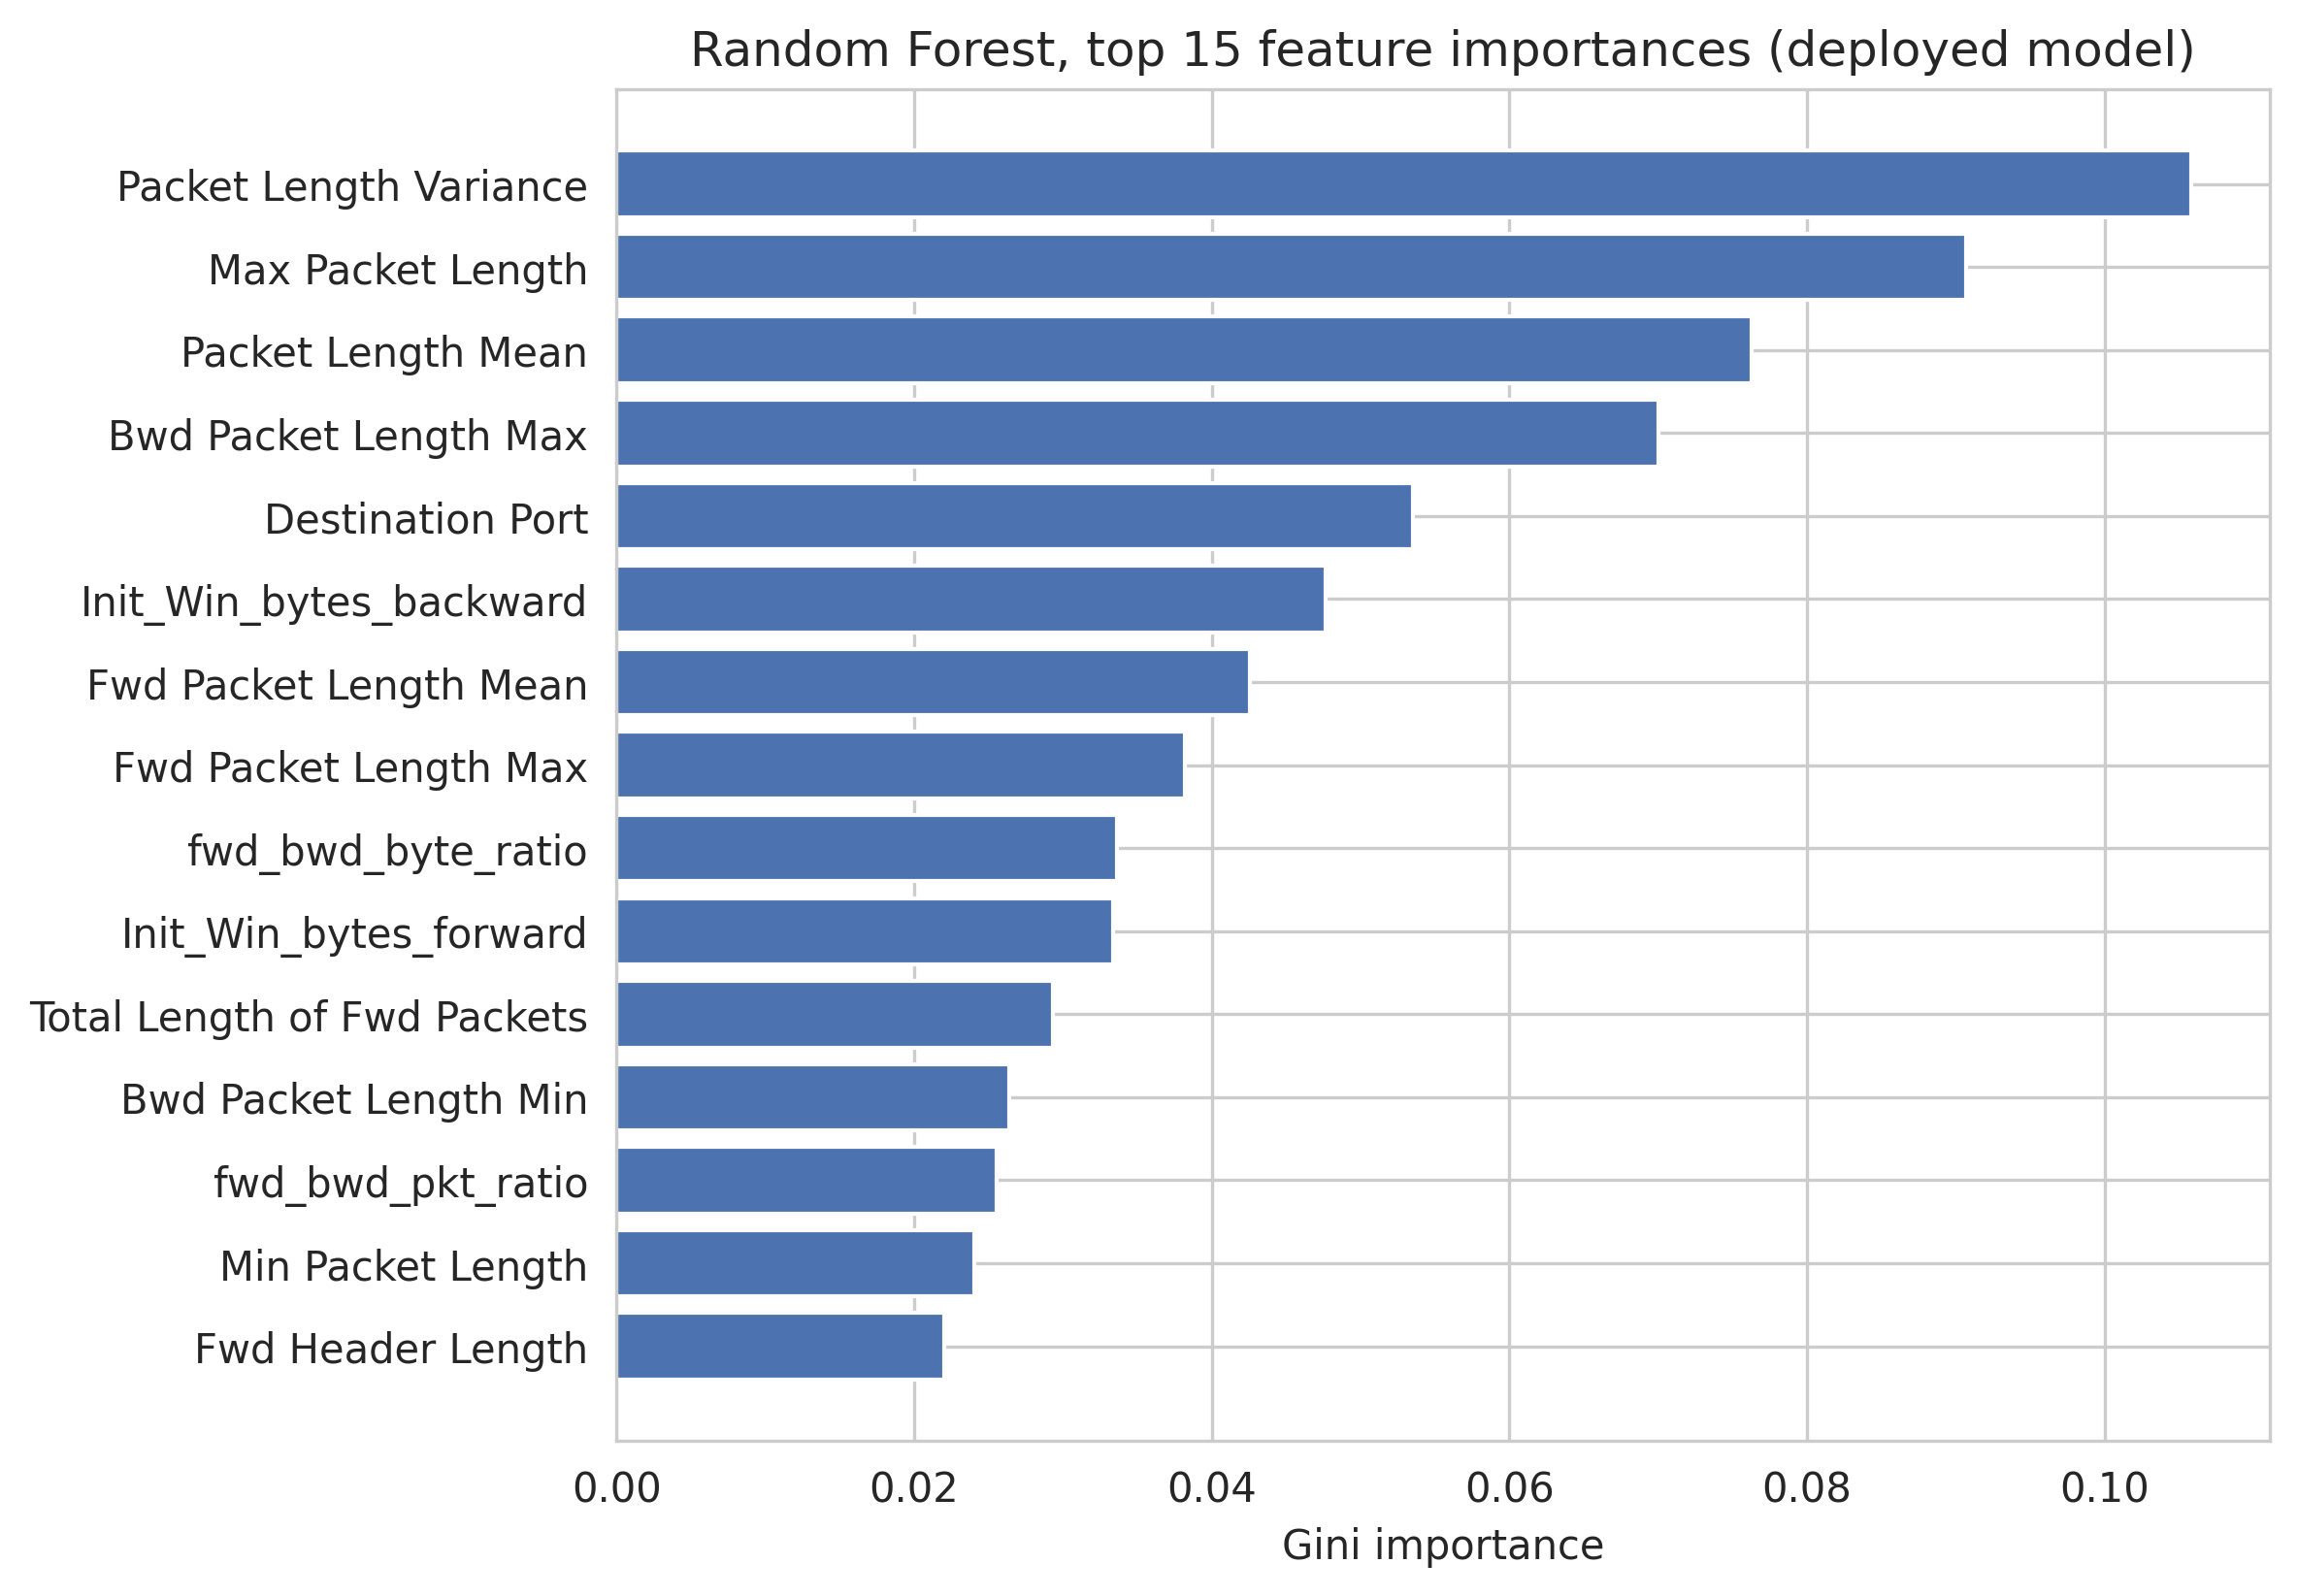
\includegraphics[width=0.85\textwidth]{figures/rf_feature_importance.png}
  \caption{Gini feature importance of the deployed Random Forest, the fifteen highest of its 49 features.}
  \label{fig:rf_importance}
\end{figure}

What SHAP effectively does is apply these ideas to the decision process in such a way as to allow a general view of how vital each feature is to the overall classification. This is what is shown in Figure~\ref{fig:shap} and at the sample size of 2000 test flows, this view agrees with the ordering of importance given by the forest model; the destination port, the forward and backward initial TCP window sizes, and packet-length derived statistics are shown to be most important. In addition, one of the two surviving engineered ratios, the forward to backward byte ratio, appears within the top ten features.

\begin{figure}[H]
  \centering
  \IfFileExists{figures/shap_summary.png}{%
    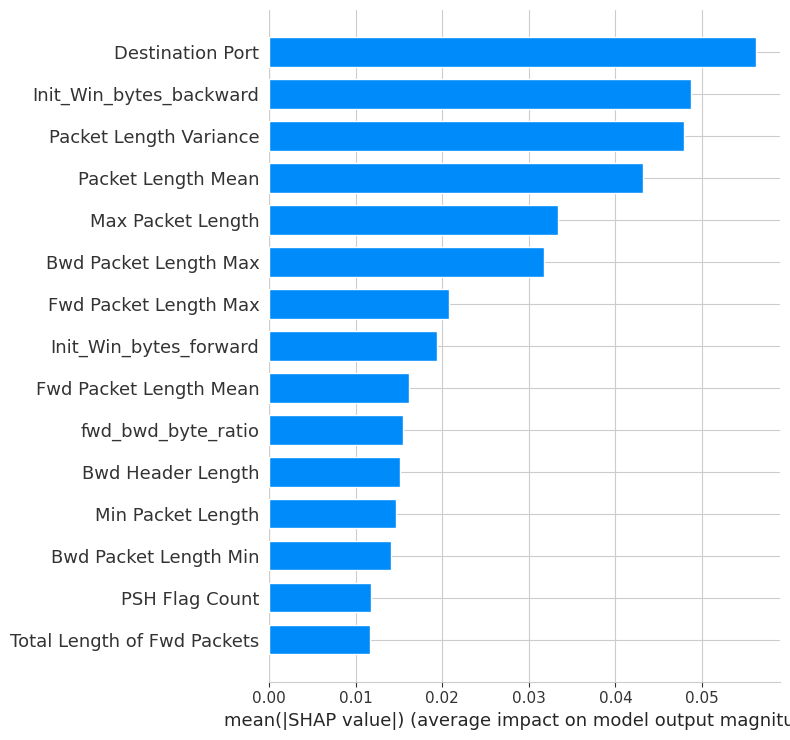
\includegraphics[width=0.85\textwidth]{figures/shap_summary.png}%
  }{%
    \fbox{\parbox{0.85\textwidth}{\centering\vspace{1.0cm}
    \texttt{[Figure: shap\_summary.png]}\\[4pt]
    \small SHAP feature-importance summary over the model's decisions,
    showing which flow features most influence the attack verdict.
    Exported from the training notebook.
    \vspace{1.0cm}}}%
  }
  \caption{SHAP feature importance summary for the trained detector.}
  \label{fig:shap}
\end{figure}


A bar chart orders features by importance, but the impact of a feature can be either positive or negative. Figure~\ref{fig:shap_beeswarm} shows a similar explanation of the data, but with the features ordered as a distribution: each point is a single flow, its horizontal position indicates how much that feature contributed to the verdict for that flow, and the color indicates the value of the feature itself. In this case, we see that the logic of the model is more understandable: a low destination-port value is indicative of an attack, while a high destination port number is indicative of benign traffic.
This matches the pattern in the dataset: attacks tend to be confined to only a handful of service ports, whereas benign traffic utilizes much higher destination port numbers.
We also see that attack flows are more likely to have high packet-length variance, and benign flows are more likely to have a large backward initial window.

This not so related yet dramatic observation requires discussion and should not have been posed as a footnote to the above figure. Destination port turns out to be the single strongest characteristic in both viewpoints, and this is actual information upon which it is reasonable to base this model; yet, also it is the feature most unlikely to be relevant to another network, since it encodes the services being attacked here, not the attack itself. This point is reconsidered in Section~\ref{sec:results_validation} with data from lab traffic.


\begin{figure}[H]
  \centering
  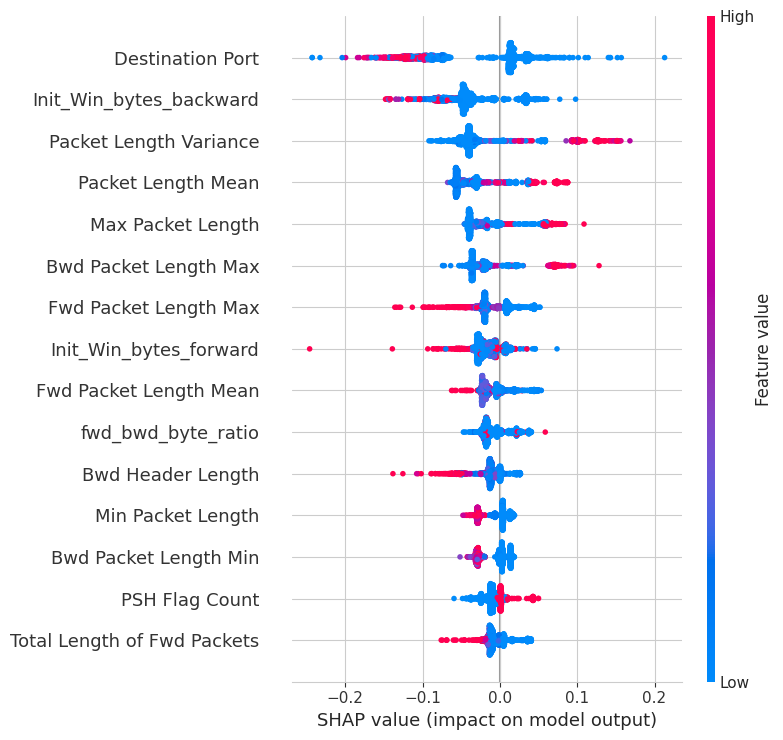
\includegraphics[width=0.85\textwidth]{figures/shap_beeswarm.png}
  \caption{SHAP values for individual flows. Each point is one flow, its colour encodes the value of the feature and its horizontal position the contribution of that feature to the attack verdict.}
  \label{fig:shap_beeswarm}
\end{figure}

In the proposed production system, these explanations would be passed to the analyst on a dashboard, which we discuss in Chapter \ref{chap:conception}. Below we apply the explainability layer to the detector itself; the analyst interface dashboard is omitted in favor of more research.

% ─────────────────────────────────────────────────────────────
\section{Validation on Independently Generated Traffic}
\label{sec:results_validation}

Everything that has been done so far is normal, good practice and culminate in a model that almost succeeds a public benchmark test. We are now faced with the question that a benchmark can not answer alone: will the model identify attacks that come at it in a format that never encountered during training. We tested the model by throwing actual attacks at it in the lab, translating them in the same representation that the model consumes, and then letting the model loose on it. That's where we have our own contribution and that's why its outcome is the only important result of this work as we consider it to be.

\subsection{From benchmark to reality: the feature pipeline}
\label{sec:results_pipeline}

To direct the lab traffic to the model, the lab traffic should first be transformed into a feature vector, i.e. Into the form of features that the model was trained on. The lab traffic is recorded using “tcpdump” in a VM, where we then process it into a flow vector format using CICFlowMeter, the exactly same recording tool as we used when generating the training data. Both the training data and lab traffic data have same definitions regarding the features they should contain.
 
There was one conflict we faced, the training file was generated using a pervious version of CICFlowMeter, the current version has different names for many columns, for example, it write “Dst Port” whereas the old version writes “Destination Port”, etc, although it computes the same quantities based on header values. After verification with both header formats of original and new generated file, we write a “renaming” file which maps current CICFlowMeter column output to original 49-feature model input format. After renaming, we regenerate three computed ratios (as mentioned in features section) exactly the same way it was used for training, and validate the columns of input features file before feeding them to the model. If there is a discrepancy in the input file format and model definition it is detected “loudly” instead of feeding the model something “silently” wrong. This rename step, although simple is in itself an interesting finding, because the very tool which define this benchmark has evolved across versions, this evolution will inevitably appear as “frictions” that a system designed to exceed the benchmarks must overcome.

\subsection{detection results Per-attack}
\label{sec:results_perattack}

The four captures are generated individually so that its corresponding label is clear: a benign browsing session, an SSH brute-force run, a full port scan, and a SYN flood. Since our captures only contain traffic from one type of attack, every flow in each capture is by construction labelled, which is desirable as an analyst might not want to label a million-flow capture. Finally we feed these individual captures through the learned detector and register the percentage of flows it identified in each one, shown in Table~\ref{tab:per-attack-results}.

\begin{table}[H]
  \centering
  \caption{Detection results on independently generated lab traffic.}
  \label{tab:per-attack-results}
  \renewcommand{\arraystretch}{1.3}
  \begin{tabularx}{\textwidth}{Xrrrrr}
    \toprule
    \textbf{Traffic type} & \textbf{Flows} & \textbf{Flagged} & \textbf{Rate (\%)} & \textbf{Mean prob.} & \textbf{Max prob.} \\
    \midrule
    Benign traffic     & 21            & 0 & 0.00  & 0.148 & 0.160 \\
    SSH brute force    & 6             & 4 & 66.67 & 0.488 & 0.695 \\
    Port scan          & 65,537        & 0 & 0.00  & 0.000 & 0.270 \\
    SYN flood (DoS)    & 1,523,389     & 0 & 0.00  & 0.058 & 0.150 \\
    \bottomrule
  \end{tabularx}
\end{table}

Another thing to note is that each capture was recorded separately, meaning the attack type acts as a ground-truth label on each flow. The benign row therefore reports false positives, while the attack rows report detections. The model did not identify any on the benign traffic which means no false positives on this dataset.

The last two columns show the attack probability the model assigned, not only the decision it reached. This is interesting because it shows that the misses are nowhere near the decision threshold. On a review of over 1.5 million flood flows, the maximum attack probability was 0.150 and for 65,537 scan flows, was 0.270.
These are well below the decision threshold of 0.5, and the operating point of 0.340 of Table~\ref{tab:operating_points}.
As such, these false negatives would not have been recovered, even if the threshold was reduced. There appears to be no hesitation in relation to the traffic, the model clearly has confidence that it is benign.

The proposed detector is being effective by not forcing false alarms and thus, not mistakenly classifying the normal network traffic as malicious activity. The previous statement refers to the criticism of the operation noise as the second part of Chapter~\ref{chap:ids} concerning the false alarms that commercial detectors create when carrying out their normal work.

Regarding \textbf{SSH brute force} the model correctly predicted four of six flows. This number should be considered a qualitative estimate rather than quantitative since the sample size of six flows is very small. The trend in the results though is most important as this was the only type of attack to demonstrate any transferability at all.
The reason is most likely structural.
The brute-force attack class in the training data consisted of complete login sequences, and the Hydra traces look similar to this training data. Enough similarity is preserved for the model to react, albeit weakly, with its confidence marginally above the decision threshold.

This pairing of the detector with an explainer allows an investigation into how a flow is being flagged instead of simply recording that it has been flagged. Figure~\ref{fig:shap_local} employs the SHAP layer outlined in Section~\ref{sec:results_shap} to examine the top-scoring brute-force flow, and this explanation extends the previous text. The most important factor contributing to the change of moving the base value 0.5 to the verdict of 0.695 is that the destination port is 22, whereas the packet-shape features oppose this.
This indicates that the similarity that makes this transfer attack possible is mostly due to the port – strongly linked to attacks within the training set – rather than the shape of the authentication exchange.
Also, this is the first working demonstration of the alerting behaviour designed in Section~\ref{sec:conception_realtime}, where an alert arrives with its explanation attached, in terms of the flow features that produced it.

\begin{figure}[H]
  \centering
  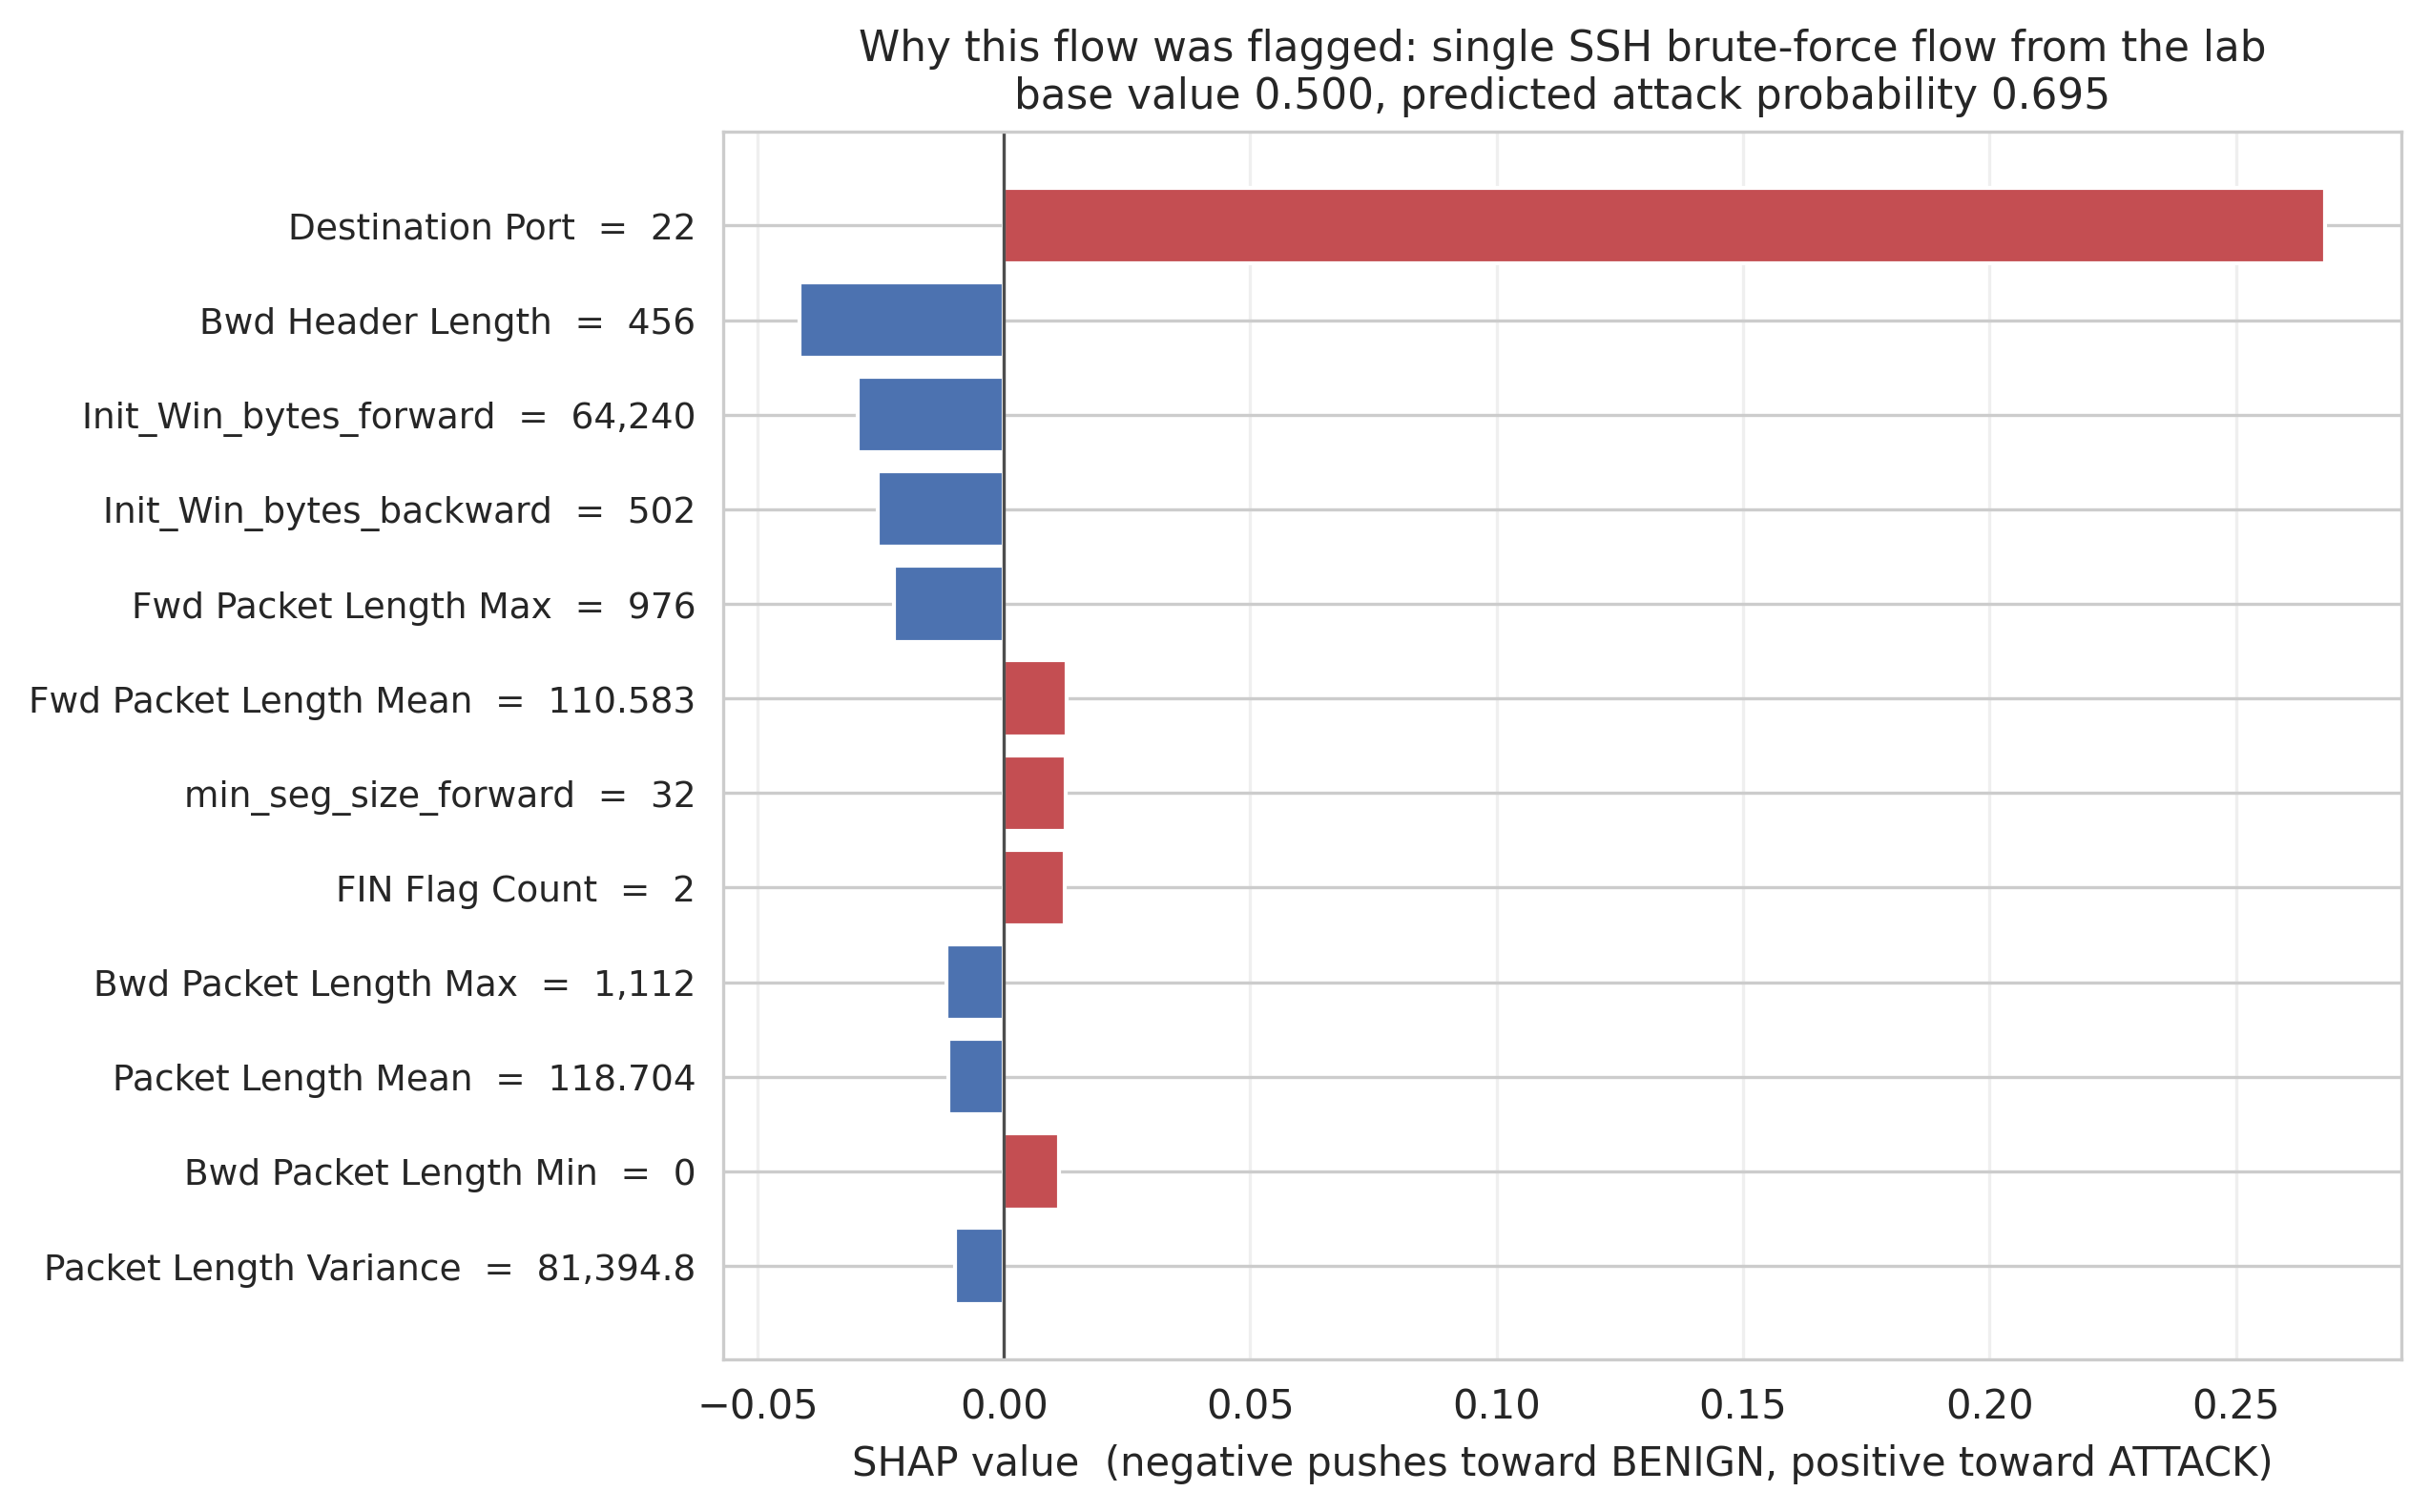
\includegraphics[width=0.9\textwidth]{figures/shap_local_ssh_flow.png}
  \caption{Per-alert explanation for one flagged SSH brute-force flow from the laboratory. Red bars push the verdict toward attack, blue bars toward benign.}
  \label{fig:shap_local}
\end{figure}

The model was entirely blind to both the \textbf{port scan} and the \textbf{SYN flood}, reporting zero detections across all sixty-five thousand scan flows and zero across the more than one and a half million flood flows. These are not marginal misses; they are total. A model that scores $0.997$ on the benchmark detected none of two high-volume attacks generated a few metres away. Understanding why is the focus of the section that follows.

\subsection{Analysis of the generalization gap}
\label{sec:results_gap}

This failure is not arbitrary, nor is it a bug in the pipeline - the features were computed and aligned correctly and valid data was passed to the model; there's a single clear reason for the failure, and the failure teaches us something about benchmarks, not this specific model.

Another example of a flow representation is SYN flood or port scan, which consists of only one packet sent to a target that does not connect. A single packet with a SYN flag, no reply, zero duration, 1 forward direction, and zero backward direction. CICFlowMeter correctly classifies both cases as flow, and therefore a million-packet SYN flood generates a million one-packet flows, mostly empty.
Impact of the training data It is interesting to note that application-level floods in the training data from CICIDS-2017 involve finished connections with application level requests and responses, multi-packet flows, a finite duration and specific rates. Therefore a denial of service attack will be more likely to follow this pattern. On the other hand, single packet SYN without duration looks like a very short benign connection stub that is likely to be allowed by this system.

There is, from the evidence found, a difference between the hping3 SYN flood and the DoS attack CICIDS-2017, even though the former has been provided as an identifier of the latter in the operation level in which the model works. The same is observed in the case of port scans, where the nmap SYN scan differs from the one used in the benchmarks, as the flow was built differently and the model was trained on it.
The one sentence in English that contains all rows in Table~\ref{tab:per-attack-results} is: The model can recognize attacks whose properties are expressed by rich multi-packet flows but cannot recognize attacks whose properties are expressed by slim single-packet flows. Further, this sentence also explains the benign cases, the partial-transfer of SSH, and the two total omissions.

\begin{figure}[H]
  \centering
  \IfFileExists{figures/generalization_gap.png}{%
    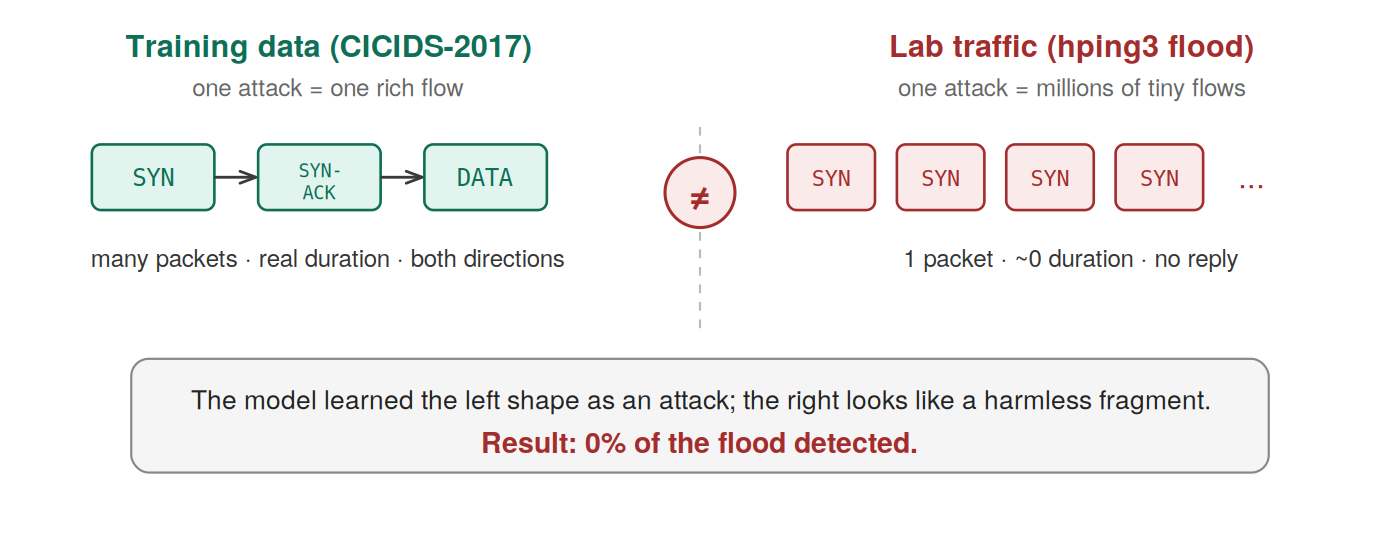
\includegraphics[width=0.95\textwidth]{figures/generalization_gap.png}%
  }{%
    \fbox{\parbox{0.85\textwidth}{\centering\vspace{1.0cm}
    \texttt{[Figure: generalization\_gap.png]}\\[4pt]
    \small Why the volumetric attacks were missed. Training taught
    ``DoS = rich multi-packet HTTP flood''; the lab produced
    single-packet SYN floods with near-zero duration. Same name,
    different flow structure, hence no detection.
    \vspace{1.0cm}}}%
  }
  \caption{The generalization gap: benchmark attacks and lab attacks that share a name but not a flow structure.}
  \label{fig:gen_gap}
\end{figure}

Our findings seem to establish that the current work has yielded important results. In particular, that we have recreated with traffic data traces owned by us one of the most well-known weaknesses of benchmark-trained intrusion detection systems: that high benchmark performance may not be indicative of high performance in real systems. While this argument has been made before in the research literature, in this work we have validated its occurrence, quantified its extent over a range of attacks, and traced it to a particular problem with flow representation.

% ─────────────────────────────────────────────────────────────
\section{Discussion}
\label{sec:results_discussion}

The result can be divided into 2 categories. The successful and unsuccessful approach. Based on the result, the model has been able to choose the most efficient and accurate model and achieved a state-of-the-art score on the benchmark.
Additionally, the model does not give any false positive on the benign traffic captured in the laboratory, while also providing explanations to its prediction with SHAP.
One disadvantage of the model is that it does not identify the volumetric attack we generate and we do know why.

There is one identified specific solution and one generic non-specific solution, but there could be any number of other solutions. The results indicate that precisely the flood that the learned classifier misses is one that other mechanisms can detect easily. For example, one could characterize the flood of single-packet SYN packets from a single host by their sending rate, and set a rule to raise an alarm whenever there are N half-open connections/sec from a source address.
This rule would quickly detect the flood missed by the learned classifier.
Therefore, the best designs is probably a \emph{hybrid} design, combining the learned classifier for the structural attacks for which it currently works well, and a set of simple rate-based rules for the volumetric attack with large packet volume. Such hybrid designs have been used in more sophisticated detectors, and the per-attack results above indicate why the combination would be effective here.

A second solution is to bypass the training gap directly retraining not just on the benchmark but also on some of lab generated traffic. As automatically taken snapshots are obviously annotated by definition, constructing a training set from these does not require humans to go through and classify them and should result in better detection of the exact types of attack that we are failing on. It is a straight forward step forward not a new experiment.

The remaining outstanding element the streaming deployment that is described in Chapter~\ref{chap:conception} i.e. The message bus, the real-time detection service and the analyst console. Our throughput achieved about 45k of flows per second that suggests a real-time operation in practice could be achievable, with the engineering outstanding.

% ─────────────────────────────────────────────────────────────
\section{Summary}
\label{sec:results_summary}

The design outlined in chapter \ref{chap:conception} has been successfully applied and tested in this chapter. We have constructed the two-machine lab, cleaned and set up the CICIDS-2017 data, developed and picked out a representation that only uses 49 features, and selected the best from three potential model approaches. One surprising aspect of the experimental results, when compared with a prior belief about the appropriate learning model, is that a Random Forest is better than a CNN or LSTM approach for this problem and the model resource usage is considerably lower. With above near perfect classification on the benchmark data and interpretation from SHAP explaining the classification decisions, we recommend this model for future efforts.

Finally, we took that model and subjected it to the only test that we felt really mattered: experiments on a set of our own attack and benign traffic data. That model generated zero false alarms and somewhat detected SSH brute-force, but completely failed to detect both a portscan and a SYN flood, because (as flow data) neither of them has the least similarity with the kind of multi-packet attacks that were in the training set. This conclusion is arguably the main contribution of our paper: proof on our own dataset that benchmark detection performance and detection on "real" data are vastly different, and a "fix" for this problem (a rule-based hybrid method, learned from the data).



%% ── General Conclusion ───────────────────────────────────────
%% ============================================================
%%  General Conclusion
%%  Broad, project-level closing. Future work here is the
%%  high-altitude outlook; the specific technical next steps
%%  Include in main.tex as an unnumbered chapter, like the
%%  General Introduction.
%% ============================================================

\chapter*{General Conclusion and Perspectives}
\addcontentsline{toc}{chapter}{General Conclusion and Perspectives}
\markboth{General Conclusion and Perspectives}{}

We had multiple objectives all focused on the idea of building a learning intrusion detection system appropriate for a cloud environment  learning feature space representations of attacks as opposed to predefined signature patterns of the same attacks, running efficiently on cheaper commodity hardware rather than inside expensive vendor locked platforms, providing explanations rather than simple report formatted output, and scanning real traffic, rather than performing analysis on masses of static data files. We authored chapters on the background to this topic, the architecture we designed for such a system, and lastly the implementation and testing of the detection core itself.

The outcome of the research has been a functioning detector. We have produced an imbalance aware, learning ready dataset based on CICIDS-2017 \cite{sharafaldin2018cicids}, reduced it to 49 flow features for the purpose of comparing different models, have tested a series of 3 differing models and met the requirement of the comparison being an "apples to apples" compare. The simple Random Forest model has been deemed the best choice; it reached an F1 score against the test set of $0.997$ at a throughput of roughly 45{,}000 flows per second, and is configured with SHAP \cite{lundberg2017shap} in order to output an explanation for each and every prediction deemed as an attack.

In conclusion, a far more important insight has been gained that is of even more value than our scores against benchmark training data. On traffic generated independently in our own laboratory, the detector returned the whole network as clear on a normal load test (no false positives) and partially detected an SSH brute force    and yet it failed on 100\% of the two high volume test loads, the port scan and the SYN flood, due to a fundamental representation problem. Both high volume test loads consisted of rapid series of minimal single packet flows. The CICIDS-2017 dataset we trained our classifier with was abundant with data gathered from multi packet traffic, which the classifier learned as the representative shape; it determined our two simple traffic structures as uninteresting, and did not classify them as malicious.

Measured against the initial objectives, the first three are met in full  a learning based detector, deployable on commodity virtualisation, explaining every alert    while the fourth is met in its core: detection was validated at real time capable throughput, with the streaming deployment specified as a design and deliberately left to future work.

This we consider the most significant finding of this work. The disparity found in our analysis (high test benchmark, low real life effectiveness) has been present throughout security machine learning research, yet it has rarely been identified explicitly. In this report, we have quantified this behavior, reasoned why it takes shape attack by attack, and traced its cause to the mismatch in flow level representation between the benchmark's attack implementations and our own. For the sake of proving the point, we have established that a calculated $0.997$ benchmark cannot be read as evidence of real world effectiveness, along with a complete classification based rationale for why the various types of malicious traffic went unidentified in a real world situation.

The current study allows us to make 3 significant suggestions of future research topics: (1) An integrated model based upon real time streaming rate monitoring combined with the learned classifier, to create our very own real world, combined shape and volume based anomaly detection. (2) Real world laboratory work to create truly applicable training datasets based solely on our own real traffic data generated within our labs, labelled by construction and requiring no manual annotation. (3) Taking our developed core technology forward to an entire real time system, along with an analyst interface.

Our own learning from this research points to a fundamental fact underlying these future directions: if a detection core can be nearly flawless against a representative public benchmark and still miss entire categories of attack generated a few metres away, then the focus on enhanced learning algorithms alone stands to question. Instead, one must identify the critical problem, which is our current method of generating training datasets    currently our greatest barrier to creating successful, useful and applicable real time learning based threat analysis security software.



\appendix
%% ============================================================
%%  Appendix A - CICFlowMeter Feature Reference
%%  The complete 79-feature list, grouped by family, with a
%%  short definition of each. Referenced from Chapter 5, §5.4.
%%  Definitions follow how CICFlowMeter computes each quantity;
%%  the handful of bulk/subflow features are defined from the
%%  tool's computation, as their official documentation is terse.
%%  Include with \appendix then \input, or \input directly after
%%  a \appendix command in main.tex.
%% ============================================================

\chapter{CICFlowMeter Feature Reference}
\label{app:features}

This appendix shows the all 79 features calculated by CICFlowMeter that were included, after variance filtering, in the detector presented in Chapter~\ref{chap:results}. The features are organized by family to allow a quicker comparison of their nature. Note that the directional terminology used,forward andbackward, correspond to the direction defined by CICFlowMeter (original direction of flow being from source to destination,andits reverse), while IAT refers to inter arrival time.

% ── Identifiers ──────────────────────────────────────────────
\section{Flow identifiers}
\label{app:feat_id}

\renewcommand{\arraystretch}{1.25}
\begin{tabularx}{\textwidth}{lX}
  \toprule
  \textbf{Feature} & \textbf{Definition} \\
  \midrule
  Flow ID          & Composite identifier of the flow (endpoints, ports, protocol). \\
  Source IP        & IP address that sent the first packet. \\
  Source Port      & Transport port that sent the first packet. \\
  Destination IP   & IP address that received the first packet. \\
  Destination Port & Transport port that received the first packet. \\
  Protocol         & Transport protocol number (e.g.\ 6 for TCP, 17 for UDP). \\
  Timestamp        & Time at which the flow began. \\
  \bottomrule
\end{tabularx}

\vspace{1em}
\noindent\textit{Note.} The identifier fields locate a flow but are not used as learning features by the detector; the model is trained to recognise attacks by traffic shape, not by address or port memorisation.

% ── Packet & byte counts ─────────────────────────────────────
\section{Packet and byte counts}
\label{app:feat_counts}

\begin{tabularx}{\textwidth}{lX}
  \toprule
  \textbf{Feature} & \textbf{Definition} \\
  \midrule
  Total Fwd Packets            & Number of packets in the forward direction. \\
  Total Backward Packets       & Number of packets in the backward direction. \\
  Total Length of Fwd Packets  & Sum of forward packet sizes (bytes). \\
  Total Length of Bwd Packets  & Sum of backward packet sizes (bytes). \\
  Subflow Fwd Packets          & Average number of forward packets per sub-flow. \\
  Subflow Fwd Bytes            & Average number of forward bytes per sub-flow. \\
  Subflow Bwd Packets          & Average number of backward packets per sub-flow. \\
  Subflow Bwd Bytes            & Average number of backward bytes per sub-flow. \\
  act\_data\_pkt\_fwd          & Number of forward packets carrying at least one byte of payload. \\
  \bottomrule
\end{tabularx}

% ── Packet length statistics ─────────────────────────────────
\section{Packet length statistics}
\label{app:feat_lengths}

\begin{tabularx}{\textwidth}{lX}
  \toprule
  \textbf{Feature} & \textbf{Definition} \\
  \midrule
  Fwd Packet Length Max   & Largest forward packet (bytes). \\
  Fwd Packet Length Min   & Smallest forward packet (bytes). \\
  Fwd Packet Length Mean  & Mean forward packet size. \\
  Fwd Packet Length Std   & Standard deviation of forward packet size. \\
  Bwd Packet Length Max   & Largest backward packet (bytes). \\
  Bwd Packet Length Min   & Smallest backward packet (bytes). \\
  Bwd Packet Length Mean  & Mean backward packet size. \\
  Bwd Packet Length Std   & Standard deviation of backward packet size. \\
  Min Packet Length       & Smallest packet in the flow, either direction. \\
  Max Packet Length       & Largest packet in the flow, either direction. \\
  Packet Length Mean      & Mean packet size over the whole flow. \\
  Packet Length Std       & Standard deviation of packet size over the flow. \\
  Packet Length Variance  & Variance of packet size over the flow. \\
  Average Packet Size     & Mean size of all packets in the flow. \\
  Avg Fwd Segment Size    & Mean forward segment (payload) size. \\
  Avg Bwd Segment Size    & Mean backward segment (payload) size. \\
  min\_seg\_size\_forward  & Minimum forward segment size observed. \\
  \bottomrule
\end{tabularx}

% ── Timing ───────────────────────────────────────────────────
\section{Flow timing and inter-arrival times}
\label{app:feat_timing}

\begin{tabularx}{\textwidth}{lX}
  \toprule
  \textbf{Feature} & \textbf{Definition} \\
  \midrule
  Flow Duration   & Total lifetime of the flow (microseconds). \\
  Flow IAT Mean   & Mean gap between successive packets in the flow. \\
  Flow IAT Std    & Standard deviation of that gap. \\
  Flow IAT Max    & Largest gap between successive packets. \\
  Flow IAT Min    & Smallest gap between successive packets. \\
  Fwd IAT Total   & Total time between forward packets. \\
  Fwd IAT Mean    & Mean gap between forward packets. \\
  Fwd IAT Std     & Standard deviation of the forward gap. \\
  Fwd IAT Max     & Largest gap between forward packets. \\
  Fwd IAT Min     & Smallest gap between forward packets. \\
  Bwd IAT Total   & Total time between backward packets. \\
  Bwd IAT Mean    & Mean gap between backward packets. \\
  Bwd IAT Std     & Standard deviation of the backward gap. \\
  Bwd IAT Max     & Largest gap between backward packets. \\
  Bwd IAT Min     & Smallest gap between backward packets. \\
  \bottomrule
\end{tabularx}

% ── Active/idle ──────────────────────────────────────────────
\section{Active and idle periods}
\label{app:feat_activeidle}

\begin{tabularx}{\textwidth}{lX}
  \toprule
  \textbf{Feature} & \textbf{Definition} \\
  \midrule
  Active Mean & Mean time the flow was active before going idle. \\
  Active Std  & Standard deviation of active periods. \\
  Active Max  & Longest active period. \\
  Active Min  & Shortest active period. \\
  Idle Mean   & Mean time the flow was idle before becoming active again. \\
  Idle Std    & Standard deviation of idle periods. \\
  Idle Max    & Longest idle period. \\
  Idle Min    & Shortest idle period. \\
  \bottomrule
\end{tabularx}

% ── TCP flags ────────────────────────────────────────────────
\section{TCP flag counts}
\label{app:feat_flags}

\begin{tabularx}{\textwidth}{lX}
  \toprule
  \textbf{Feature} & \textbf{Definition} \\
  \midrule
  Fwd PSH Flags   & Count of PSH flags on forward packets. \\
  Bwd PSH Flags   & Count of PSH flags on backward packets. \\
  Fwd URG Flags   & Count of URG flags on forward packets. \\
  Bwd URG Flags   & Count of URG flags on backward packets. \\
  FIN Flag Count  & Count of FIN flags in the flow. \\
  SYN Flag Count  & Count of SYN flags in the flow. \\
  RST Flag Count  & Count of RST flags in the flow. \\
  PSH Flag Count  & Count of PSH flags in the flow. \\
  ACK Flag Count  & Count of ACK flags in the flow. \\
  URG Flag Count  & Count of URG flags in the flow. \\
  CWE Flag Count  & Count of CWR (congestion-window-reduced) flags in the flow. \\
  ECE Flag Count  & Count of ECE (ECN-echo) flags in the flow. \\
  \bottomrule
\end{tabularx}

% ── Header & rates ───────────────────────────────────────────
\section{Header lengths, rates, and ratios}
\label{app:feat_rates}

\begin{tabularx}{\textwidth}{lX}
  \toprule
  \textbf{Feature} & \textbf{Definition} \\
  \midrule
  Fwd Header Length        & Total bytes used by forward packet headers. \\
  Bwd Header Length        & Total bytes used by backward packet headers. \\
  Flow Bytes/s             & Bytes per second over the flow's lifetime. \\
  Flow Packets/s           & Packets per second over the flow's lifetime. \\
  Fwd Packets/s            & Forward packets per second. \\
  Bwd Packets/s            & Backward packets per second. \\
  Down/Up Ratio            & Ratio of backward (download) to forward (upload) traffic. \\
  \bottomrule
\end{tabularx}

% ── Bulk & window ────────────────────────────────────────────
\section{Bulk-transfer and connection-window features}
\label{app:feat_bulk}

\begin{tabularx}{\textwidth}{lX}
  \toprule
  \textbf{Feature} & \textbf{Definition} \\
  \midrule
  Fwd Avg Bytes/Bulk    & Average bytes per forward bulk-transfer burst. \\
  Fwd Avg Packets/Bulk  & Average packets per forward bulk-transfer burst. \\
  Fwd Avg Bulk Rate     & Average rate of forward bulk transfer. \\
  Bwd Avg Bytes/Bulk    & Average bytes per backward bulk-transfer burst. \\
  Bwd Avg Packets/Bulk  & Average packets per backward bulk-transfer burst. \\
  Bwd Avg Bulk Rate     & Average rate of backward bulk transfer. \\
  Init\_Win\_bytes\_forward   & Initial TCP window size advertised in the forward direction. \\
  Init\_Win\_bytes\_backward  & Initial TCP window size advertised in the backward direction. \\
  \bottomrule
\end{tabularx}

\vspace{1em}

\noindent\textit{Note on bulk features.} A ”bulk” is a series of data sending packets back-to-back all going in the same direction. CICFlowMeter calculates such counts on consecutive streaks of data sending packets, if there are no long periods of sending data on the flow these are often zero, which is why several of them get filtered out by the variance filter in Section~\ref{sec:results_features}.

% ── Engineered ───────────────────────────────────────────────
\section{Engineered features}
\label{app:feat_engineered}

The three features below are generated not by CICFlowMeter but by us by calculating counts from above (as in Section \ref{sec:results_features}), which will be replicated perfectly on live data.


\noindent\begin{tabularx}{\textwidth}{lX}
  \toprule
  \textbf{Feature} & \textbf{Definition} \\
  \midrule
  fwd\_bwd\_pkt\_ratio  & Forward packet count divided by backward packet count. \\
  fwd\_bwd\_byte\_ratio & Forward byte count divided by backward byte count. \\
  avg\_fwd\_pkt\_size   & Total forward bytes divided by total forward packets. \\
  \bottomrule
\end{tabularx}

% ── Removed features ─────────────────────────────────────────
\section{Features removed during selection}
\label{app:feat_dropped}

Of the 80 candidate features available once the three engineered ratios had been added, 31 were removed before training, leaving the 49 the detector uses. Table~\ref{tab:dropped_constant} lists the eight columns whose value is identical in every flow of the prepared dataset, and Table~\ref{tab:dropped_corr} the 23 removed for redundancy, each with the retained feature it duplicates and the absolute correlation between them. The correlations are measured on a sample of 300,000 flows.

\begin{table}[H]
  \centering
  \caption{The eight zero-variance features removed by the variance filter.}
  \label{tab:dropped_constant}
  \renewcommand{\arraystretch}{1.25}
\begin{tabularx}{\textwidth}{lX}
  \toprule
  \textbf{Feature} & \textbf{Constant value} \\
  \midrule
  Bwd PSH Flags        & 0 \\
  Bwd URG Flags        & 0 \\
  Fwd Avg Bytes/Bulk   & 0 \\
  Fwd Avg Packets/Bulk & 0 \\
  Fwd Avg Bulk Rate    & 0 \\
  Bwd Avg Bytes/Bulk   & 0 \\
  Bwd Avg Packets/Bulk & 0 \\
  Bwd Avg Bulk Rate    & 0 \\
  \bottomrule
\end{tabularx}
\end{table}

\begin{table}[H]
  \centering
  \caption{The 23 features removed by the correlation filter, with the retained feature each duplicates.}
  \label{tab:dropped_corr}
  \renewcommand{\arraystretch}{1.25}
\begin{tabularx}{\textwidth}{lXr}
  \toprule
  \textbf{Removed feature} & \textbf{Duplicates} & $|\rho|$ \\
  \midrule
  Total Backward Packets      & Total Fwd Packets           & 0.998 \\
  Total Length of Bwd Packets & act\_data\_pkt\_fwd         & 0.994 \\
  Fwd Packet Length Std       & Fwd Packet Length Max       & 0.969 \\
  Bwd Packet Length Mean      & Bwd Packet Length Max       & 0.958 \\
  Bwd Packet Length Std       & Bwd Packet Length Max       & 0.982 \\
  Fwd IAT Total               & Flow Duration               & 0.999 \\
  Fwd IAT Max                 & Flow IAT Max                & 0.998 \\
  Fwd Packets/s               & Flow Packets/s              & 0.980 \\
  Packet Length Std           & Max Packet Length           & 0.984 \\
  SYN Flag Count              & Fwd PSH Flags               & 1.000 \\
  CWE Flag Count              & Fwd URG Flags               & 1.000 \\
  ECE Flag Count              & RST Flag Count              & 0.994 \\
  Average Packet Size         & Packet Length Mean          & 0.998 \\
  Avg Fwd Segment Size        & Fwd Packet Length Mean      & 1.000 \\
  Avg Bwd Segment Size        & Bwd Packet Length Max       & 0.958 \\
  Subflow Fwd Packets         & Total Fwd Packets           & 1.000 \\
  Subflow Fwd Bytes           & Total Length of Fwd Packets & 1.000 \\
  Subflow Bwd Packets         & Total Fwd Packets           & 0.998 \\
  Subflow Bwd Bytes           & act\_data\_pkt\_fwd         & 0.994 \\
  Idle Mean                   & Flow IAT Max                & 0.980 \\
  Idle Max                    & Flow IAT Max                & 0.990 \\
  Idle Min                    & Flow IAT Max                & 0.951 \\
  avg\_fwd\_pkt\_size         & Fwd Packet Length Mean      & 1.000 \\
  \bottomrule
\end{tabularx}
\end{table}
   % the 79-feature table
%% ============================================================
%%  Appendix B - Model Training Notebook
%%  A pointer page, not a full code dump. Describes the notebook,
%%  its structure, and where the complete version lives. Optionally
%%  includes one representative excerpt.
%%  Requires \appendix to have been called before \input.
%%  Uses listings (lstlisting); if not already loaded, add
%%  \usepackage{listings} to the preamble.
%% ============================================================

\chapter{Model Training Notebook}
\label{app:notebook}

All the steps listed that forms the entire model-training pipeline, has been developed and designed on Google Colab in a jupyter notebook (with GPU acceleration). This notebook acts as a one and only reference point to every step performed from raw-data to exported model assets and will be provided with the electronic copy of this thesis. All contents will be enumerated in this annex. The notebook name is \texttt{CICIDS2017\_training.ipynb}.

\section{Contents}
\label{app:notebook_contents}

The notebook is organised into the following stages, in execution order:

\begin{enumerate}
  \item \textbf{Environment setup} : installation of dependencies and confirmation of GPU availability.
  \item \textbf{Data loading} : reading and concatenating the six retained CICIDS-2017 files.
  \item \textbf{Cleaning} : stripping column-name whitespace, replacing infinite values, repairing corrupted labels, and removing the duplicated header column (Section~\ref{sec:results_cleaning}).
  \item \textbf{Exploratory analysis} : class distribution and feature summaries.
  \item \textbf{Feature engineering} : construction of the three engineered ratio features (Section~\ref{sec:results_features}).
  \item \textbf{Feature selection} : variance filtering to the final feature set, with the leakage-safe ordering of split, scale, and resample.
  \item \textbf{Model training} : the three candidate models (Random Forest, CNN, LSTM).
  \item \textbf{Comparison and evaluation} : the metrics of Table~\ref{tab:model_comparison}, the confusion matrix, and the precision--recall curve.
  \item \textbf{Threshold tuning} : selection of the operating point on the validation split.
  \item \textbf{Explainability} : SHAP analysis of the selected model.
  \item \textbf{Export} : serialisation of the model, the scaler, and the frozen feature order metadata.
\end{enumerate}

\section{Exported artifacts}
\label{app:notebook_artifacts}

The notebook produces the artifacts consumed by the detection pipeline of Section~\ref{sec:results_validation}:

\begin{center}
\begin{tabular}{ll}
  \toprule
  \textbf{Artifact} & \textbf{Role} \\
  \midrule
  \texttt{detector\_rf.joblib}   & The trained Random Forest classifier. \\
  \texttt{scaler.joblib}         & The fitted scaler (used by the deep models). \\
  \texttt{model\_metadata.json}  & The frozen feature order and configuration. \\
  \bottomrule
\end{tabular}
\end{center}

% \section{Availability}
% \label{app:notebook_availability}

% The full notebook, together with the exported artifacts, is available in the project repository accompanying this thesis:

% \begin{center}
% \texttt{[https://github.com/\textit{Aboubakree}/\textit{EYP-Cloud-Intrusion-Detection-AI}]}
% \end{center}

% \noindent A copy is also included in the digital submission archive.
   % the notebook
%% ============================================================
%%  Appendix C - Detection and Evaluation Scripts
%%  Pointer page describing the scripts, with ONE short
%%  representative excerpt (the feature-reconciliation logic,
%%  since that is the scientifically relevant part).
%%  Requires \appendix before \input, and \usepackage{listings}.
%% ============================================================

\chapter{Detection and Evaluation Scripts}
\label{app:scripts}

The trained model was validated against some independently generated laboratory traffic (Section~\ref{sec:results_validation}) using a small group of Python scripts. Once again the whole source for these can be found with the digital submission instead of being printed here, here I explain each script and include the one snippet of logic that the results depend on  reconciling the featureisation of the live traffic with what the model expected.

\section{Scripts}
\label{app:scripts_list}

\begin{center}
\begin{tabular}{ll}
  \toprule
  \textbf{Script} & \textbf{Purpose} \\
  \midrule
  \texttt{evaluate\_per\_attack.py}   & Produces the per-attack detection table (Table~\ref{tab:per-attack-results}). \\
  \bottomrule
\end{tabular}
\end{center}

All scripts will carry out the exact same sequence: Read CICFlowMeter output. Rename the columns to those expected in the training process. Engineer features exactly as in training.
Check that all of the needed features exist.
Only if all required features exist will the model be used. The check is intentional: if a column is missing or named incorrectly, the script will fail rather than feeding something unexpected to the model.

\section{Feature reconciliation}
\label{app:scripts_excerpt}

The only bit of this script that should not be trivial, is the mapping used to align the existing CICFlowMeter output with the feature names that the trained model expects to be in use, as the training files were generated using a previous release of the software, and some columns have since had their names changed when calculating the same value. This mapping function accounts for that discrepancy:

\begin{lstlisting}[language=Python, basicstyle=\ttfamily\small, breaklines=true, columns=fullflexible]
# CICFlowMeter (current release) -> CICIDS-2017 training names.
# Same underlying quantities; only the column labels differ.
RENAME_V4_TO_TRAIN = {
    "Dst Port":                    "Destination Port",
    "Total Fwd Packet":            "Total Fwd Packets",
    "Total Bwd packets":           "Total Backward Packets",
    "Total Length of Fwd Packet":  "Total Length of Fwd Packets",
    "Total Length of Bwd Packet":  "Total Length of Bwd Packets",
    "Packet Length Min":           "Min Packet Length",
    "Packet Length Max":           "Max Packet Length",
    "FWD Init Win Bytes":          "Init_Win_bytes_forward",
    "Bwd Init Win Bytes":          "Init_Win_bytes_backward",
    "Fwd Act Data Pkts":           "act_data_pkt_fwd",
    "Fwd Seg Size Min":            "min_seg_size_forward",
}
\end{lstlisting}

\noindent After renaming, the three engineered features are recomputed from the aligned columns, and the resulting set is checked against the frozen feature order stored in \texttt{model\_metadata.json} before any prediction is made.

\section{Availability}
\label{app:scripts_availability}

The full source of both scripts is available in the project repository accompanying this thesis:

\begin{center}
\texttt{[https://github.com/\textit{Aboubakree}/\textit{EYP-Cloud-Intrusion-Detection-AI}]}
\end{center}

\noindent and in the digital submission archive.
   % the scripts

%% ── Bibliography ─────────────────────────────────────────────
\newpage
\bibliography{references}
\addcontentsline{toc}{chapter}{References}

\end{document}
